\section{Deterministic stress tests for UniFold}
\label{sec:stressunifolddet}

Figures~\ref{fig:stressa_pT_trackj1},~\ref{fig:stressa_tau1_trackj1}, and~\ref{fig:stressa_y_trackj1} show further examples of the deterministic weight stress test for UniFold, continuing from Sec.~\ref{sec:stress:deterministic}.

\begin{figure}[h!]
\centering
\subfloat[Weights]{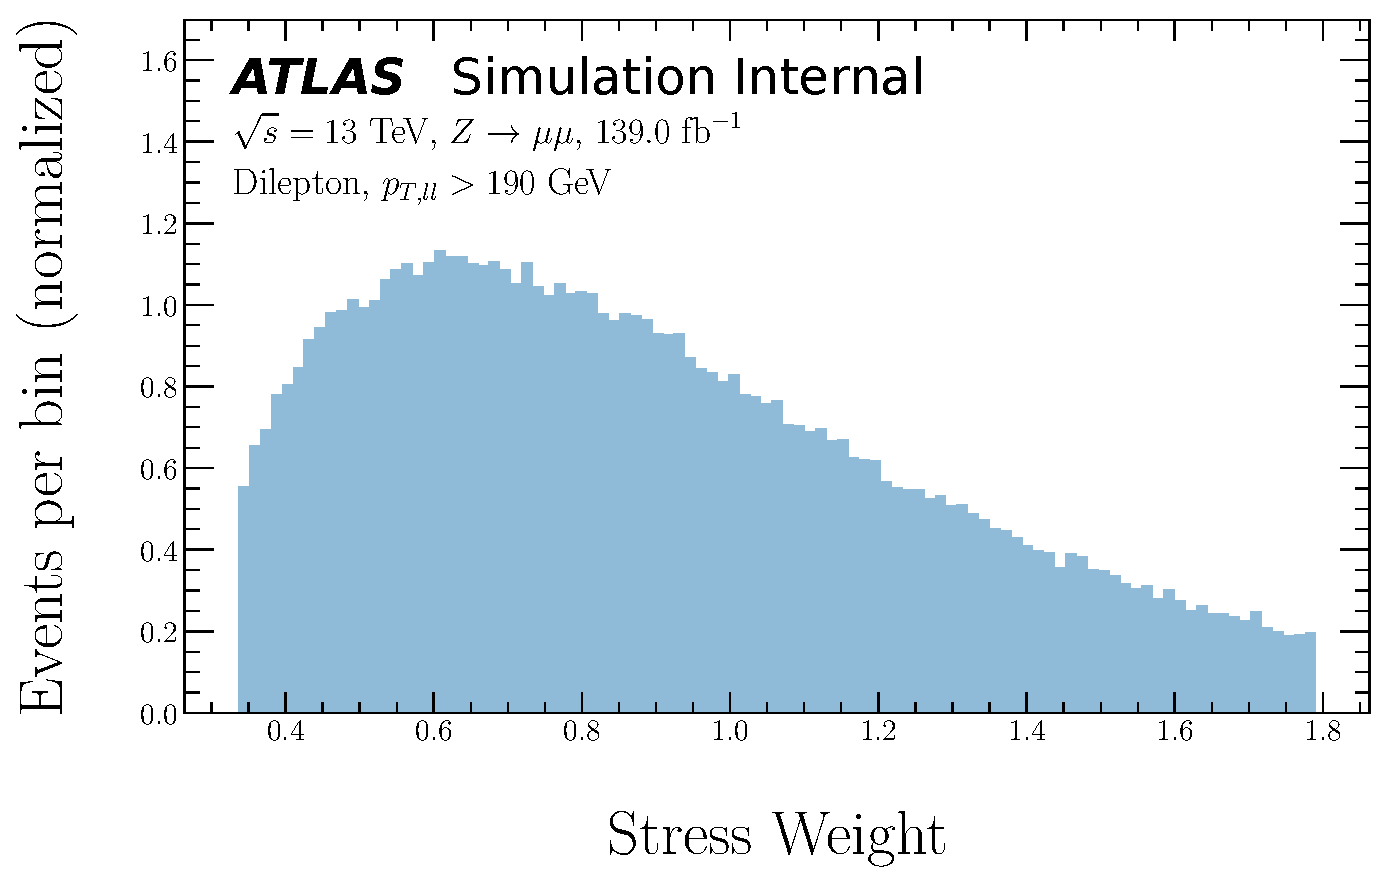
\includegraphics[width=0.45\textwidth]{figures/ATLASOmniFold-StressTest/ATLASOmniFold-StressTestA/UniFold/pT_trackj1/ATLASOmniFold-StressTestA-UniFold-pT_trackj1-StressWeightsHist.pdf}}\\
\subfloat[Input histograms]{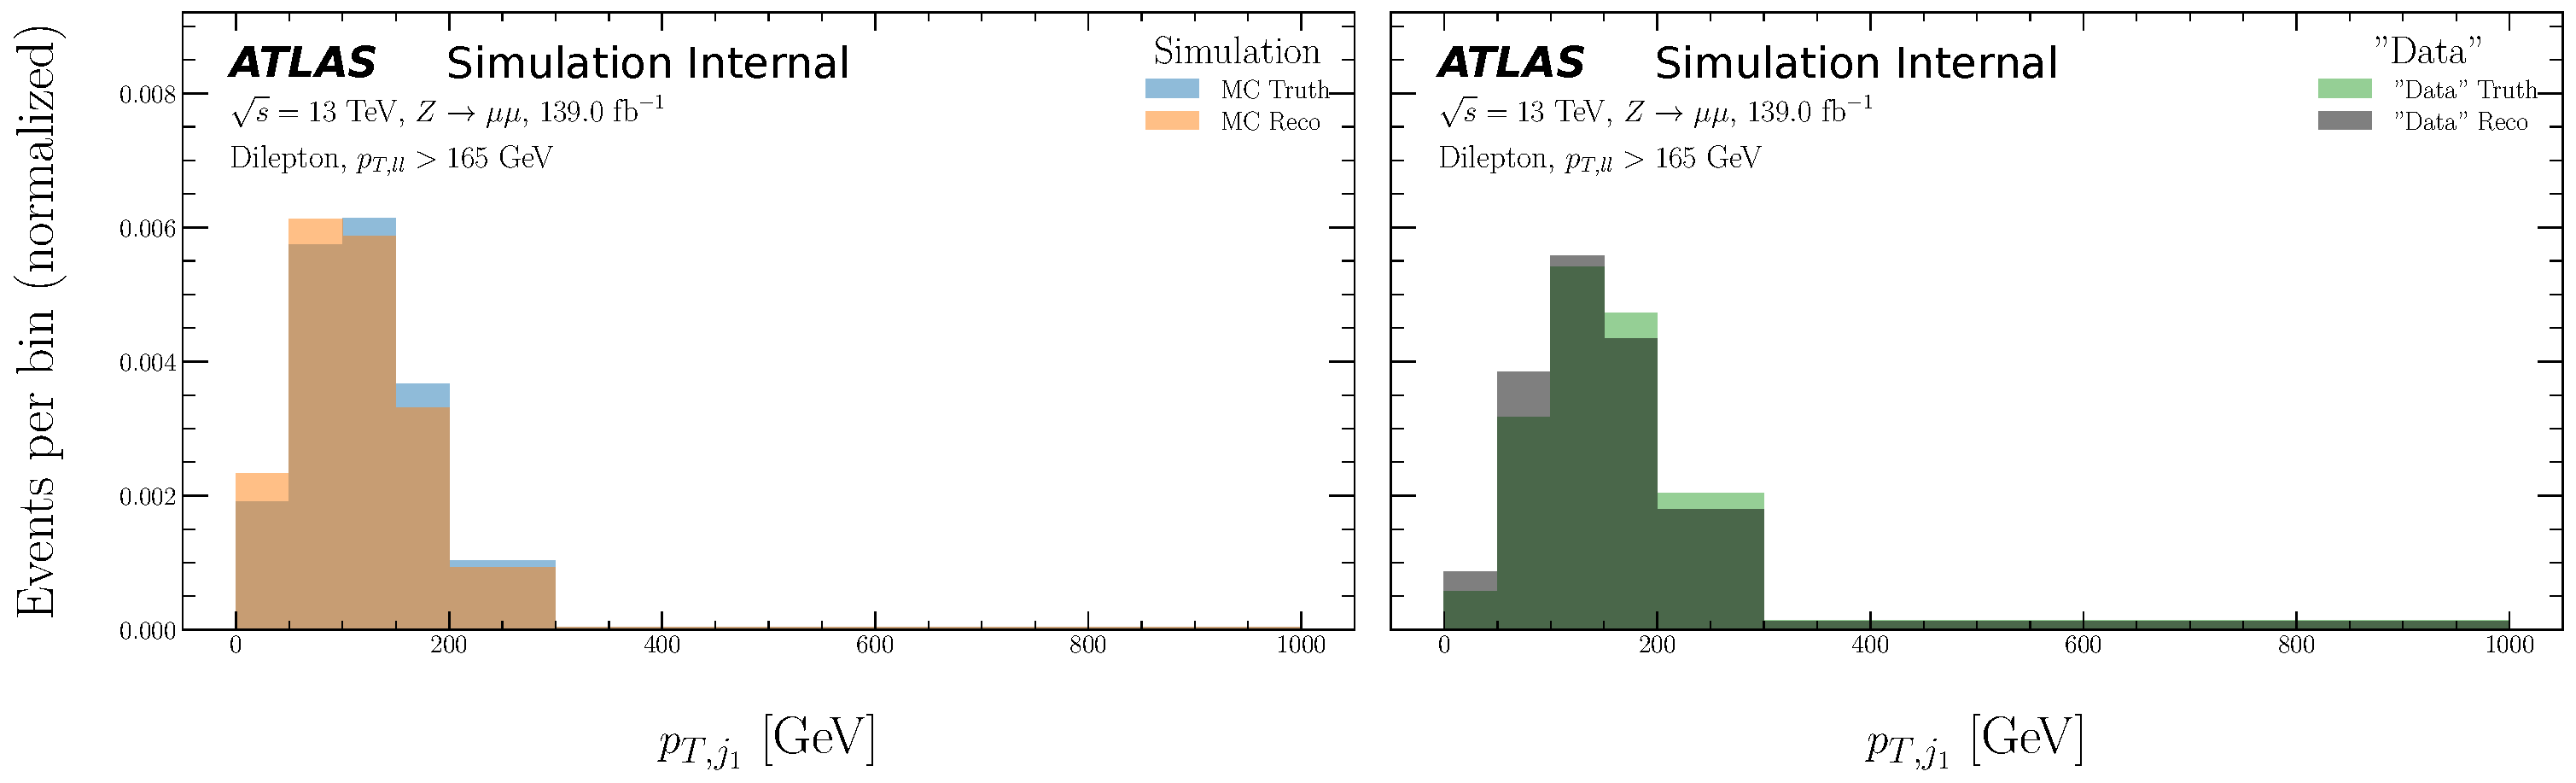
\includegraphics[width=0.85\textwidth]{figures/ATLASOmniFold-StressTest/ATLASOmniFold-StressTestA/UniFold/pT_trackj1/ATLASOmniFold-StressTestA-UniFold-pT_trackj1-Distributions}}\\
\subfloat[After 1 iteration]{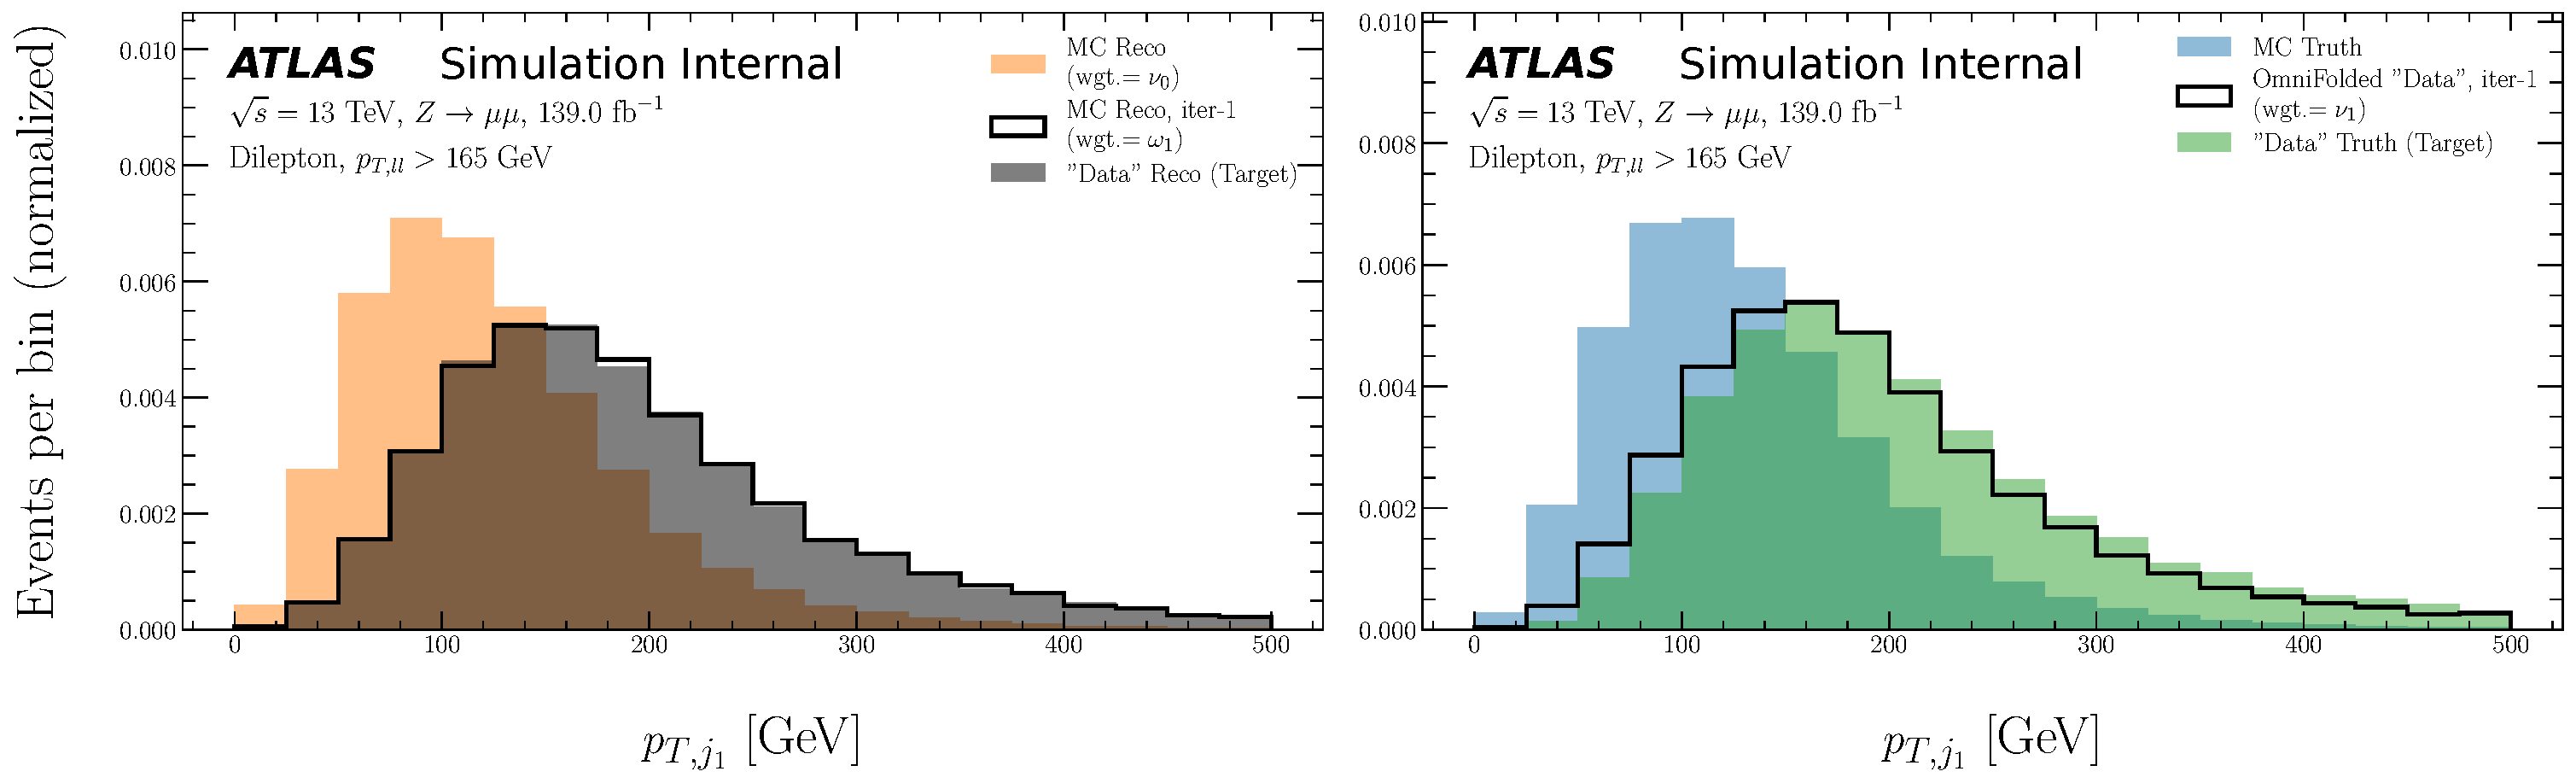
\includegraphics[width=0.85\textwidth]{figures/ATLASOmniFold-StressTest/ATLASOmniFold-StressTestA/UniFold/pT_trackj1/ATLASOmniFold-StressTestA-UniFold-pT_trackj1-Iteration01}}\\
\subfloat[After 2 iterations]{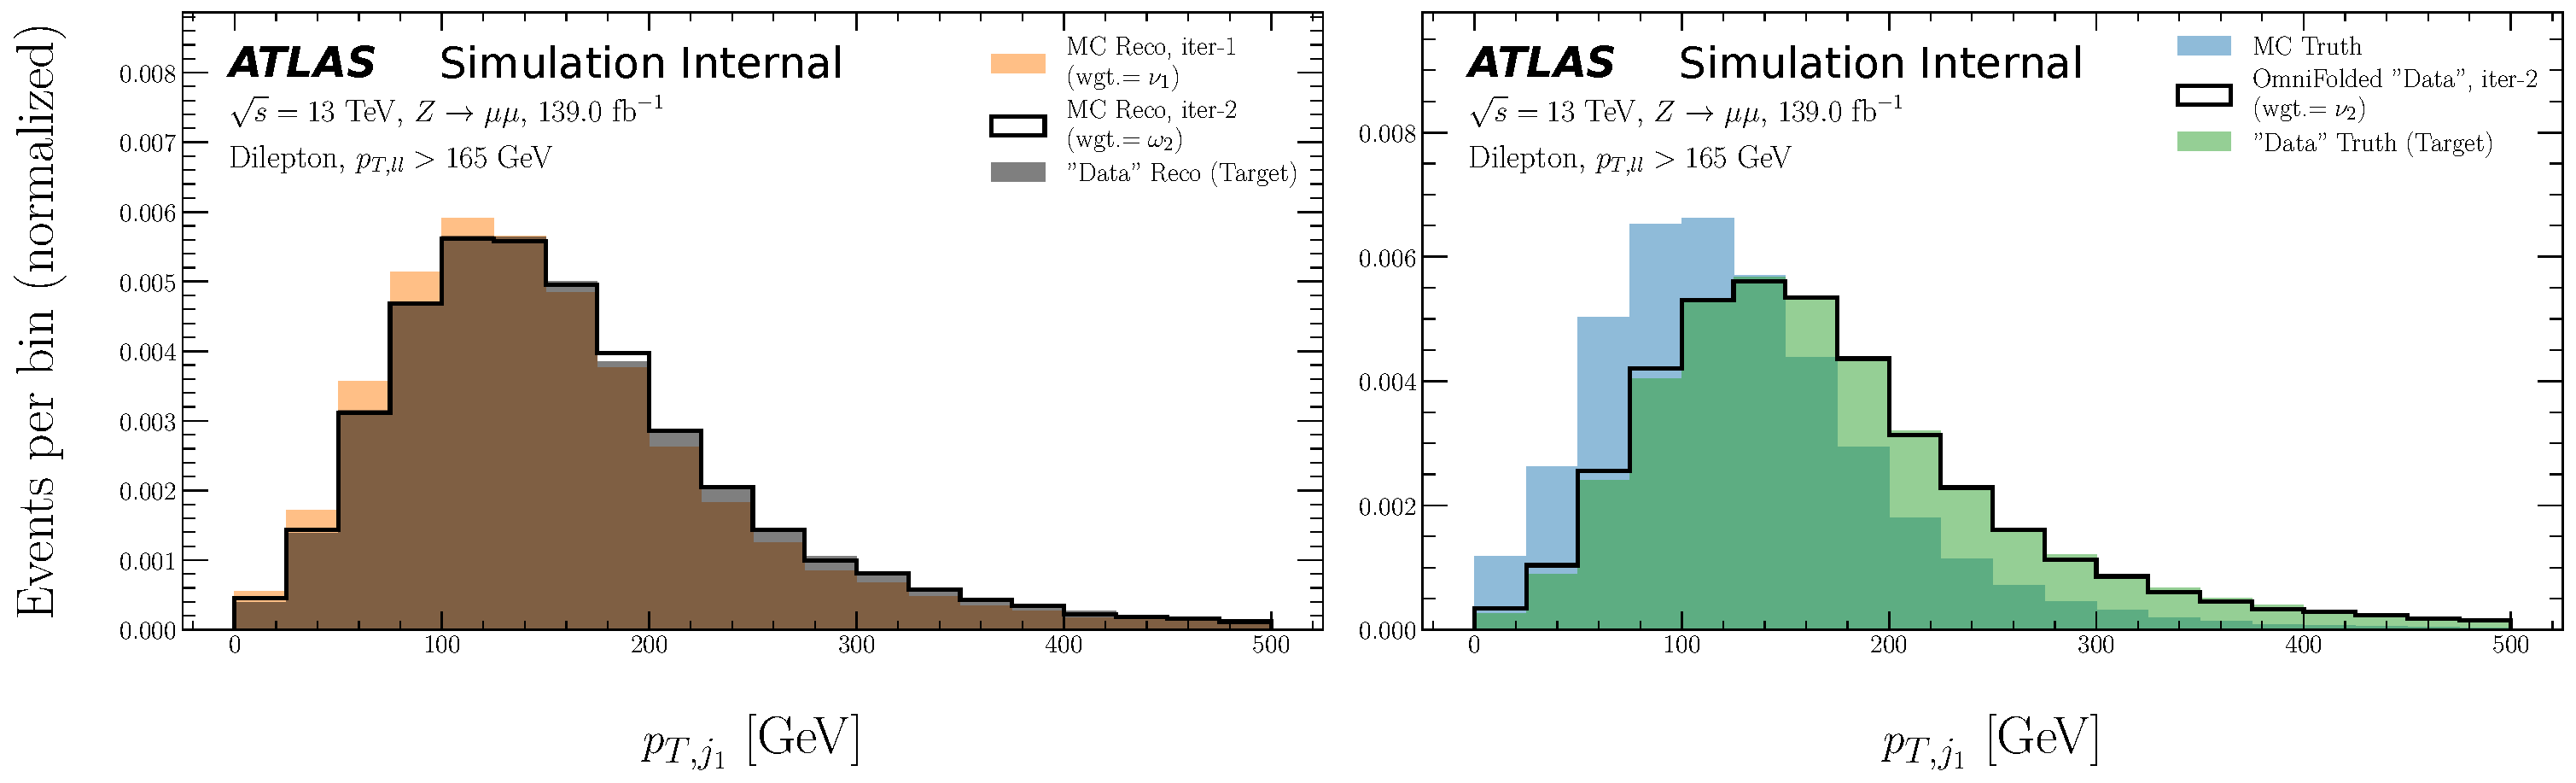
\includegraphics[width=0.85\textwidth]{figures/ATLASOmniFold-StressTest/ATLASOmniFold-StressTestA/UniFold/pT_trackj1/ATLASOmniFold-StressTestA-UniFold-pT_trackj1-Iteration02}}
\phantomcaption 
\end{figure}

\begin{figure}[h!]
\centering
\ContinuedFloat
\subfloat[After 3 iterations]{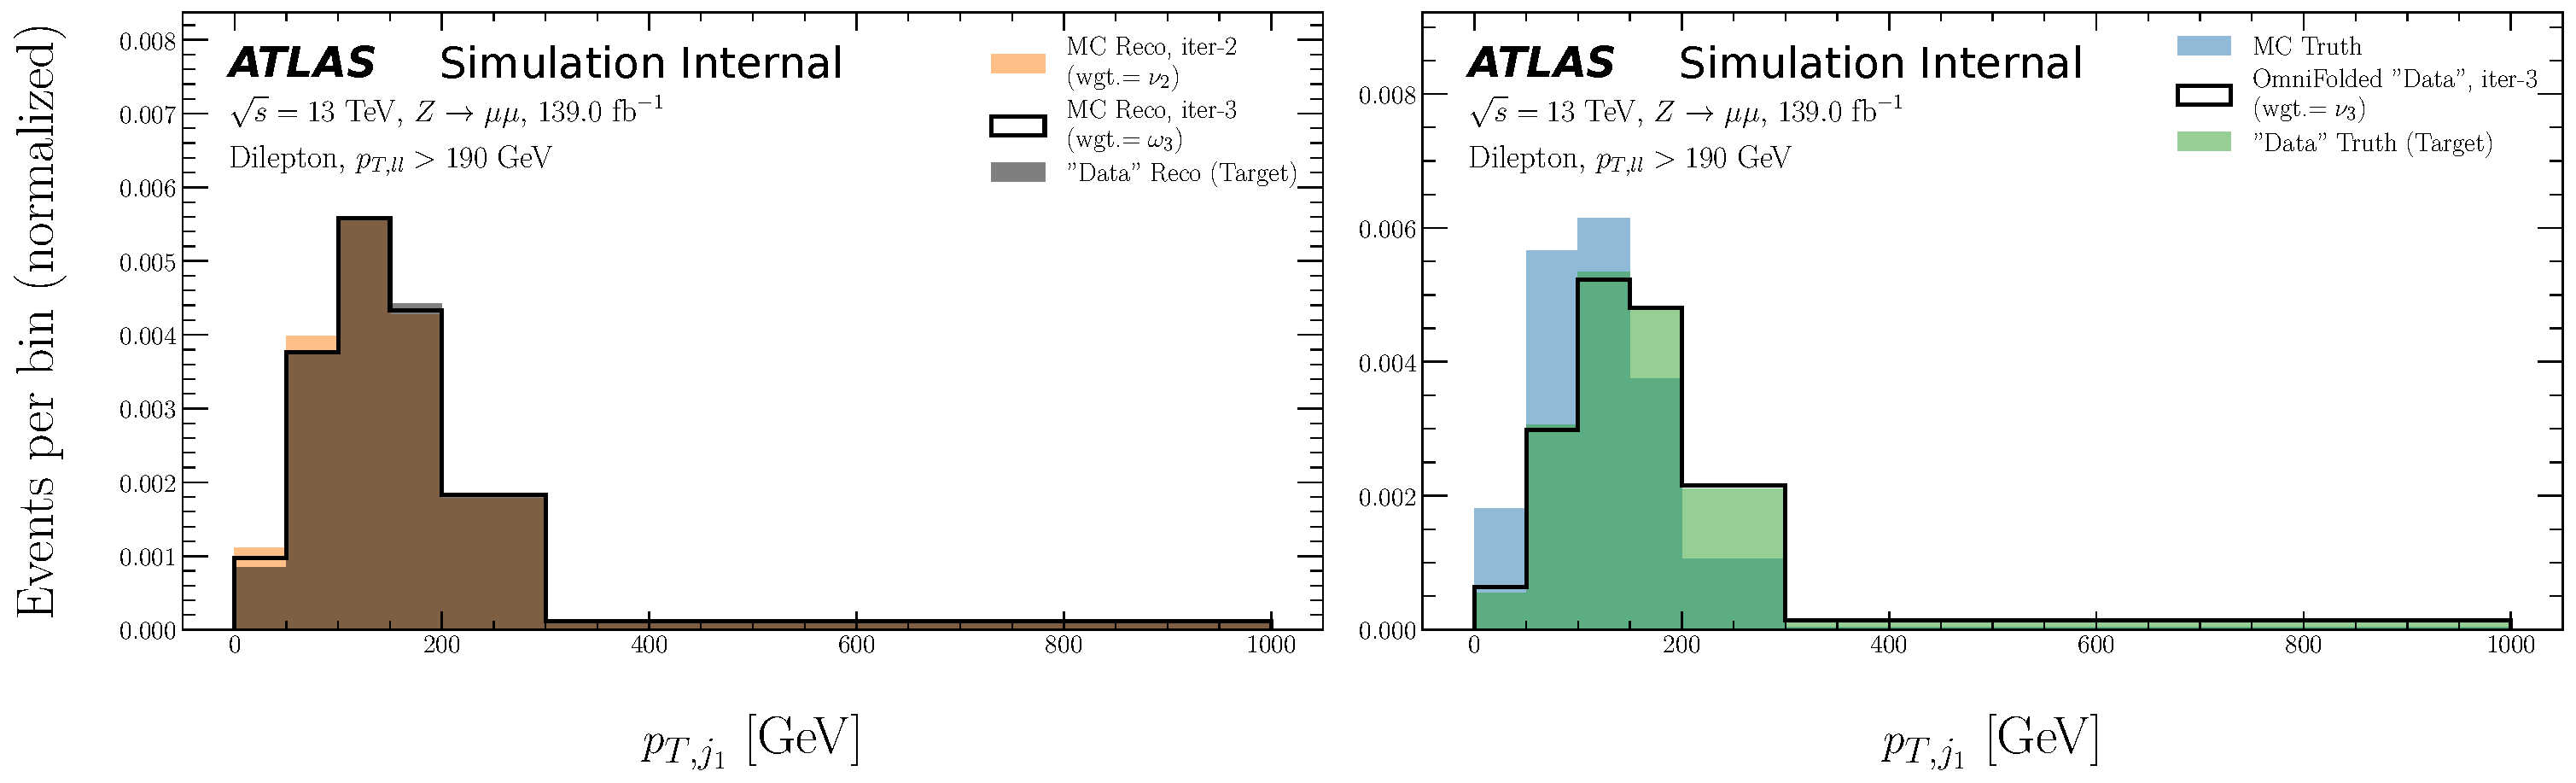
\includegraphics[width=0.85\textwidth]{figures/ATLASOmniFold-StressTest/ATLASOmniFold-StressTestA/UniFold/pT_trackj1/ATLASOmniFold-StressTestA-UniFold-pT_trackj1-Iteration03}}\\
\subfloat[After 4 iterations]{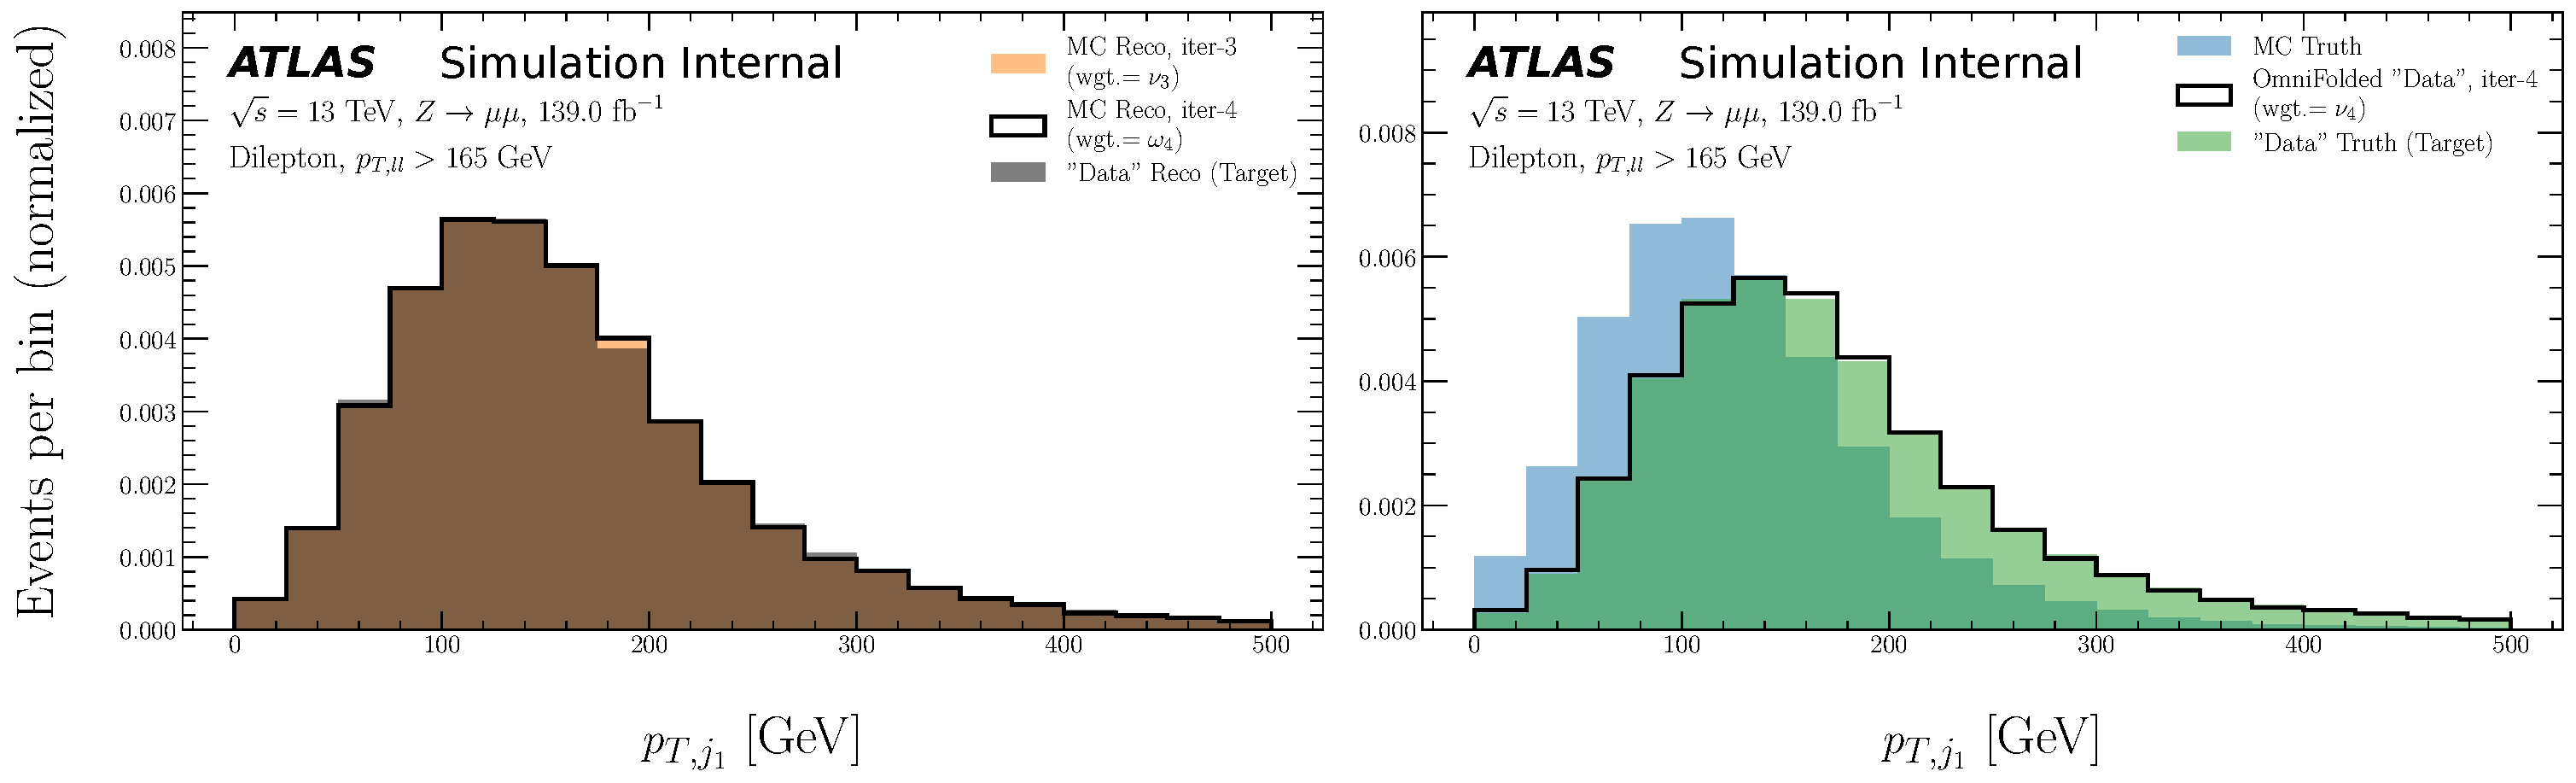
\includegraphics[width=0.85\textwidth]{figures/ATLASOmniFold-StressTest/ATLASOmniFold-StressTestA/UniFold/pT_trackj1/ATLASOmniFold-StressTestA-UniFold-pT_trackj1-Iteration04}}\\
\subfloat[After 5 iterations]{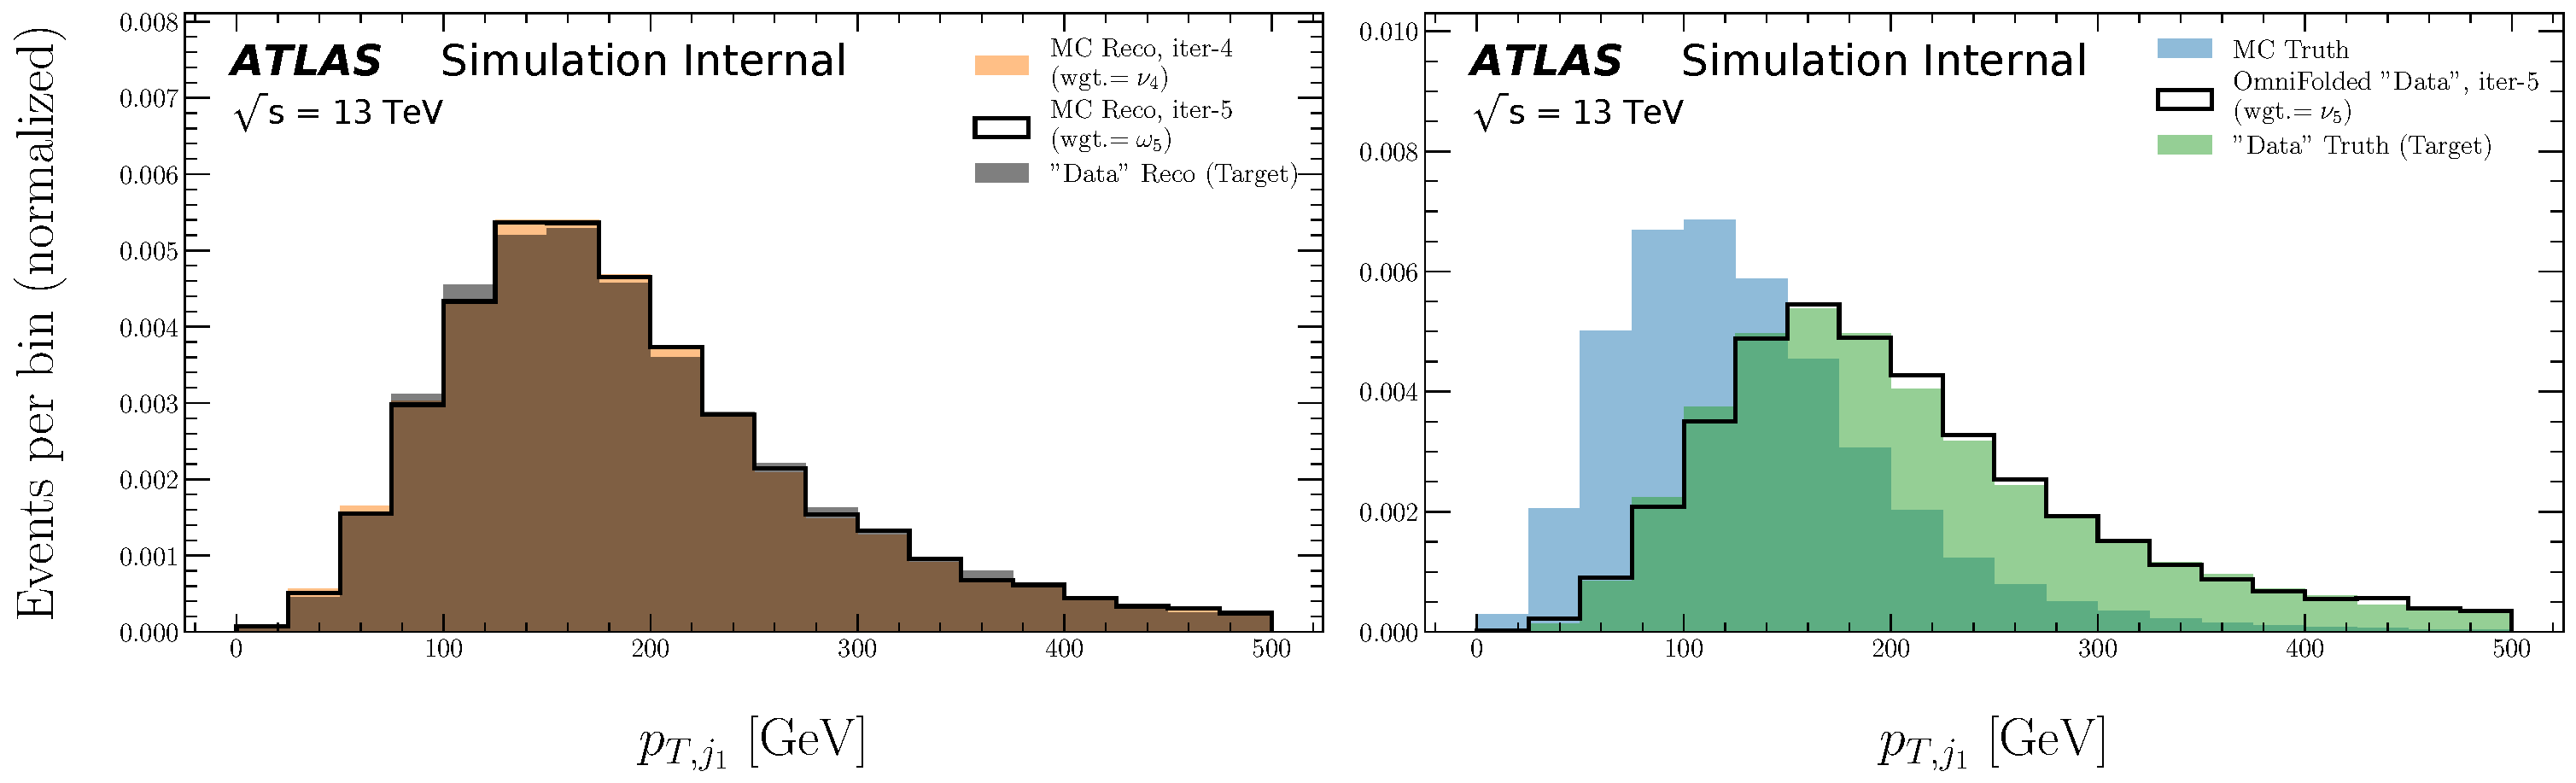
\includegraphics[width=0.85\textwidth]{figures/ATLASOmniFold-StressTest/ATLASOmniFold-StressTestA/UniFold/pT_trackj1/ATLASOmniFold-StressTestA-UniFold-pT_trackj1-Iteration05}}\\
\subfloat[After 6 iterations]{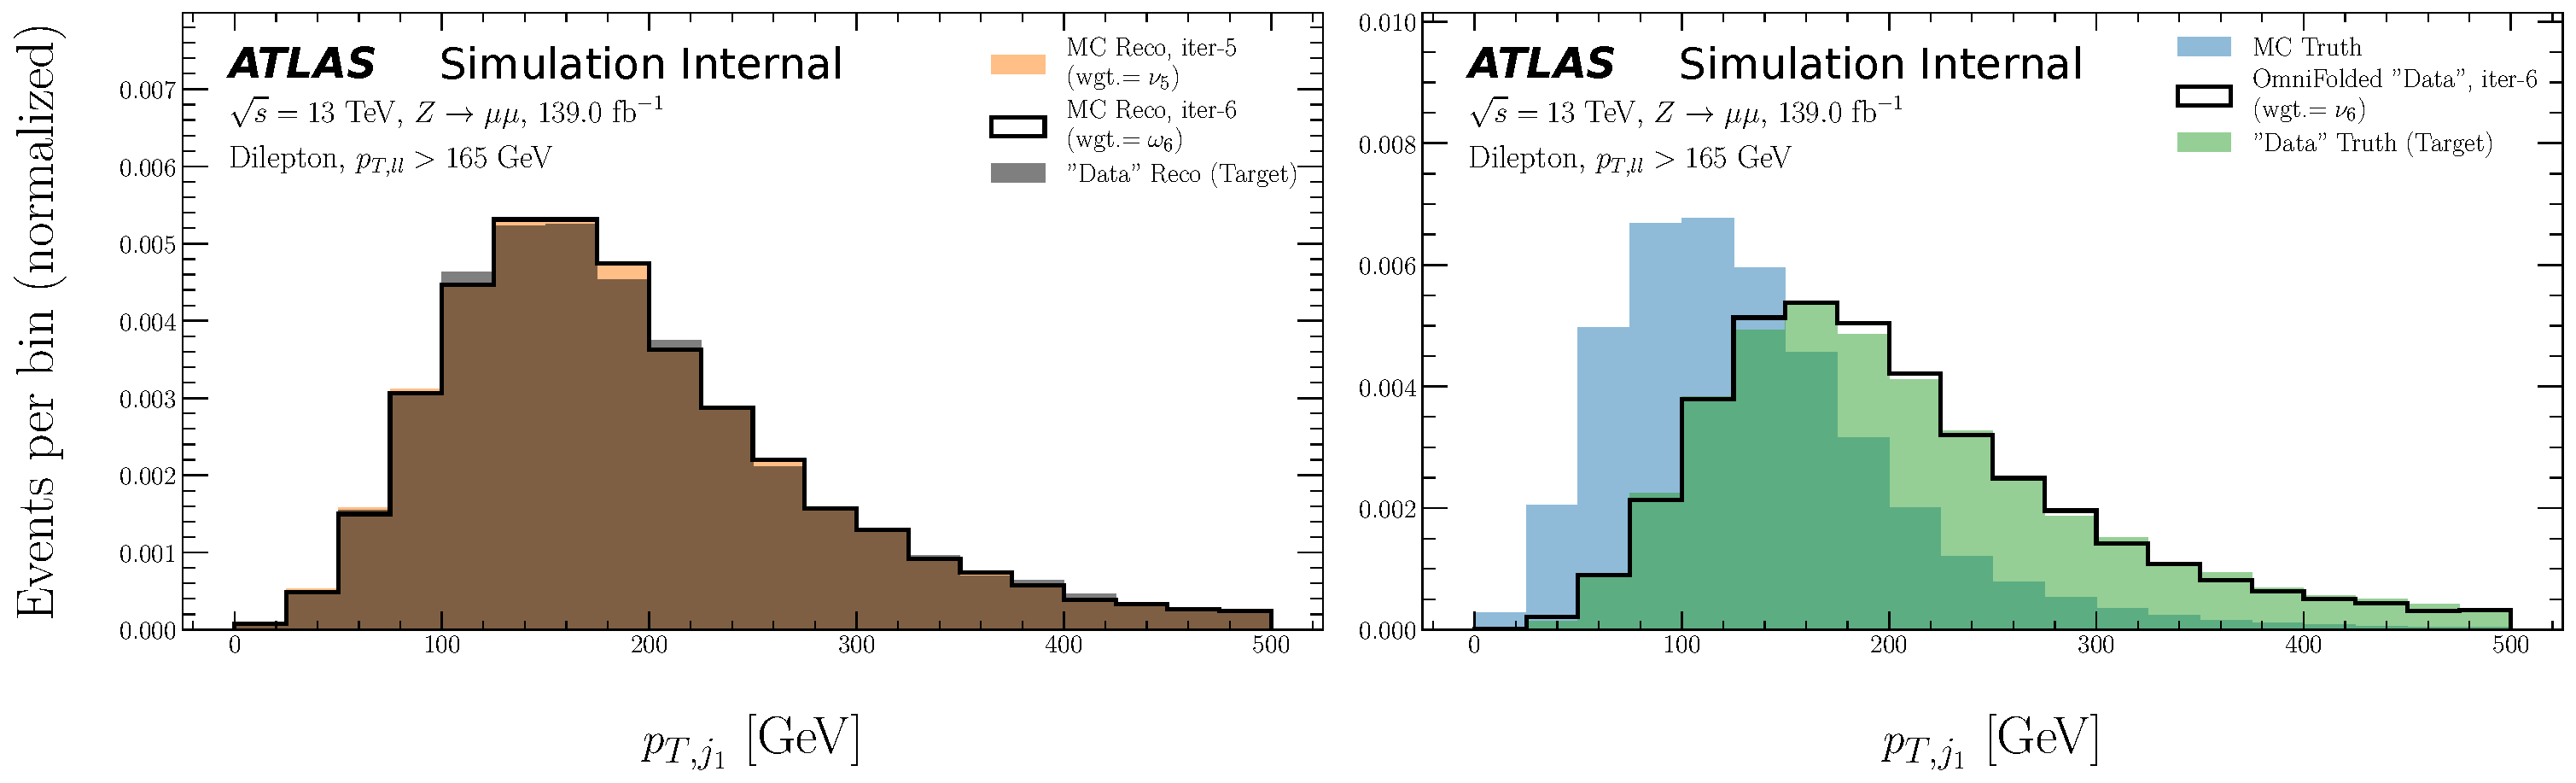
\includegraphics[width=0.85\textwidth]{figures/ATLASOmniFold-StressTest/ATLASOmniFold-StressTestA/UniFold/pT_trackj1/ATLASOmniFold-StressTestA-UniFold-pT_trackj1-Iteration06}}
\caption{A stress test for UniFold applied to the leading track jet $p_T$.}
\label{fig:stressa_pT_trackj1}
\end{figure}

\begin{figure}[h!]
\centering
\subfloat[Weights]{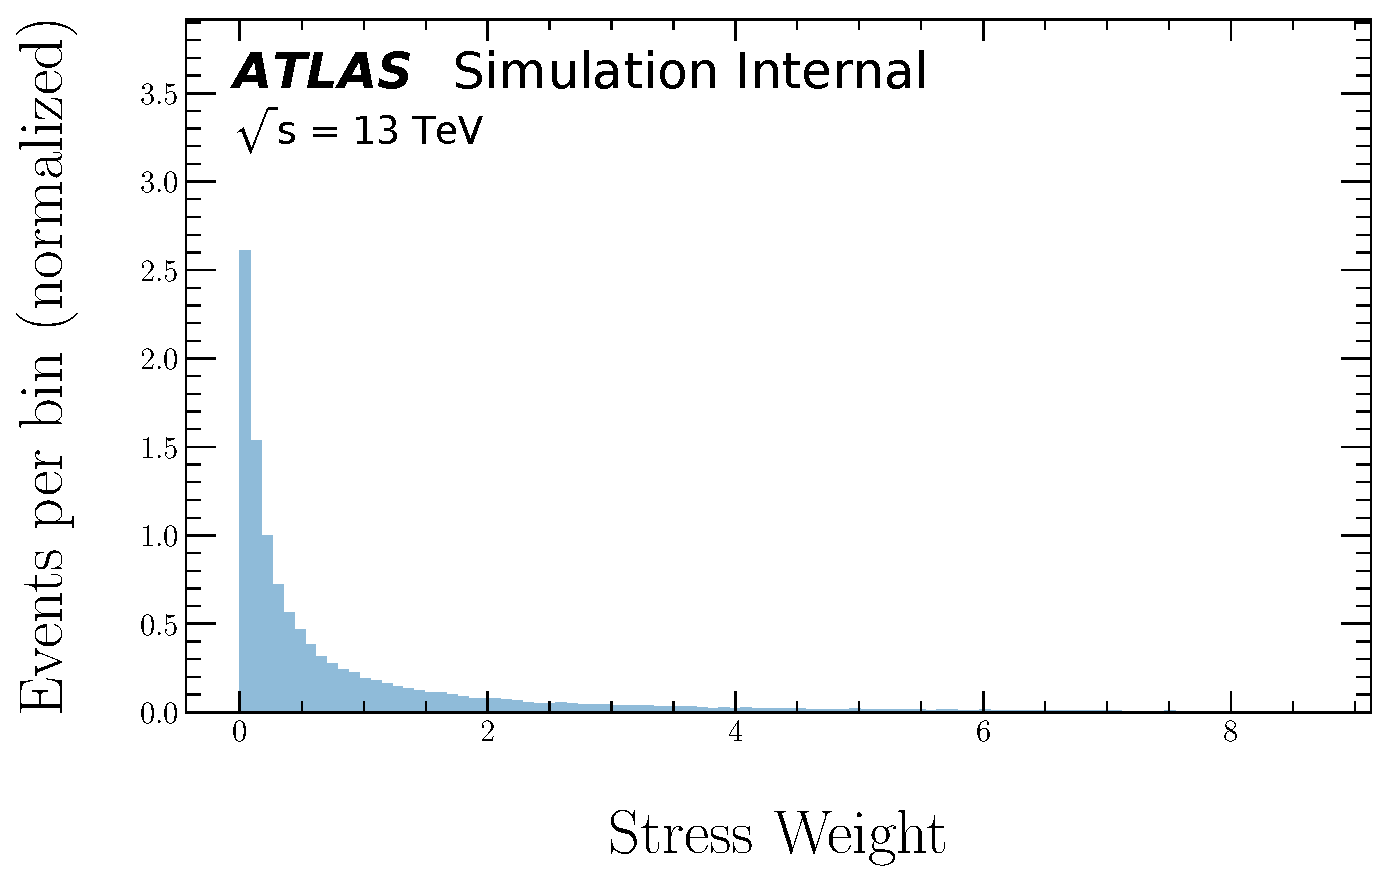
\includegraphics[width=0.45\textwidth]{figures/ATLASOmniFold-StressTest/ATLASOmniFold-StressTestA/UniFold/tau1_trackj1/ATLASOmniFold-StressTestA-UniFold-tau1_trackj1-StressWeightsHist.pdf}}\\
\subfloat[Input histograms]{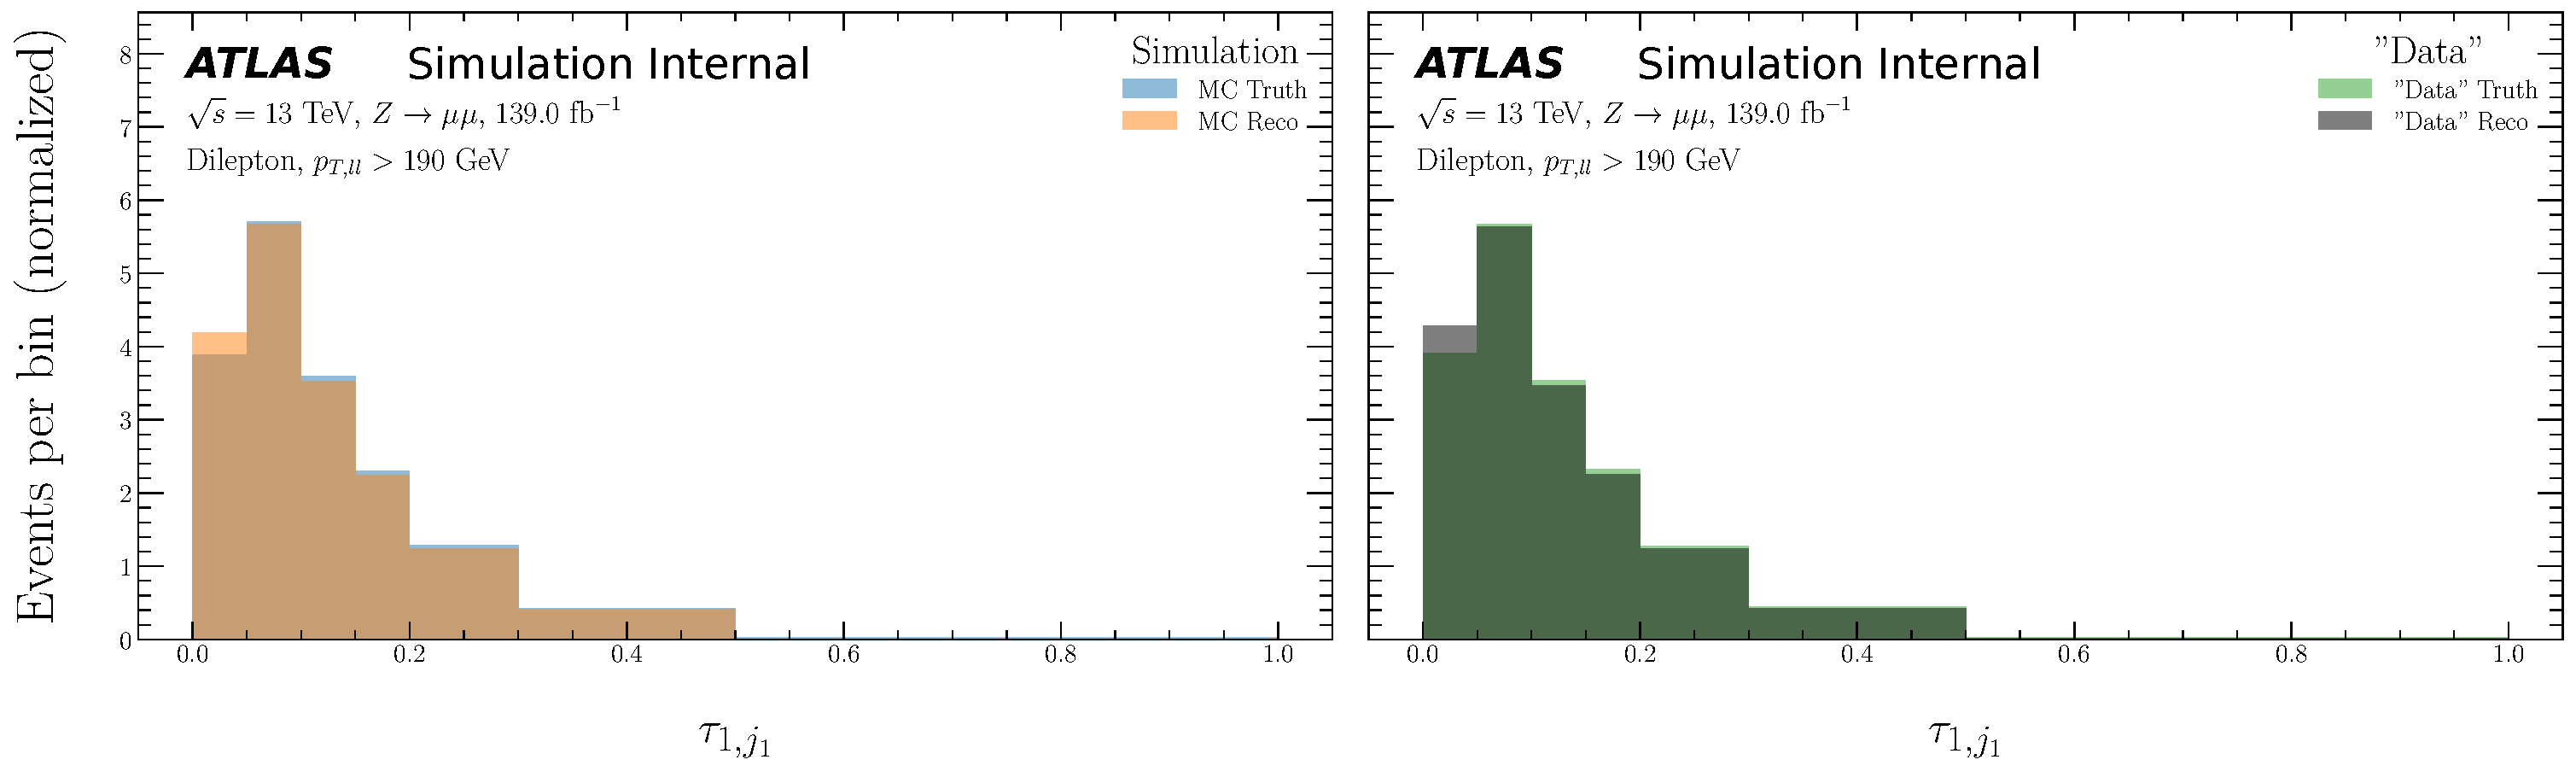
\includegraphics[width=0.85\textwidth]{figures/ATLASOmniFold-StressTest/ATLASOmniFold-StressTestA/UniFold/tau1_trackj1/ATLASOmniFold-StressTestA-UniFold-tau1_trackj1-Distributions}}\\
\subfloat[After 1 iteration]{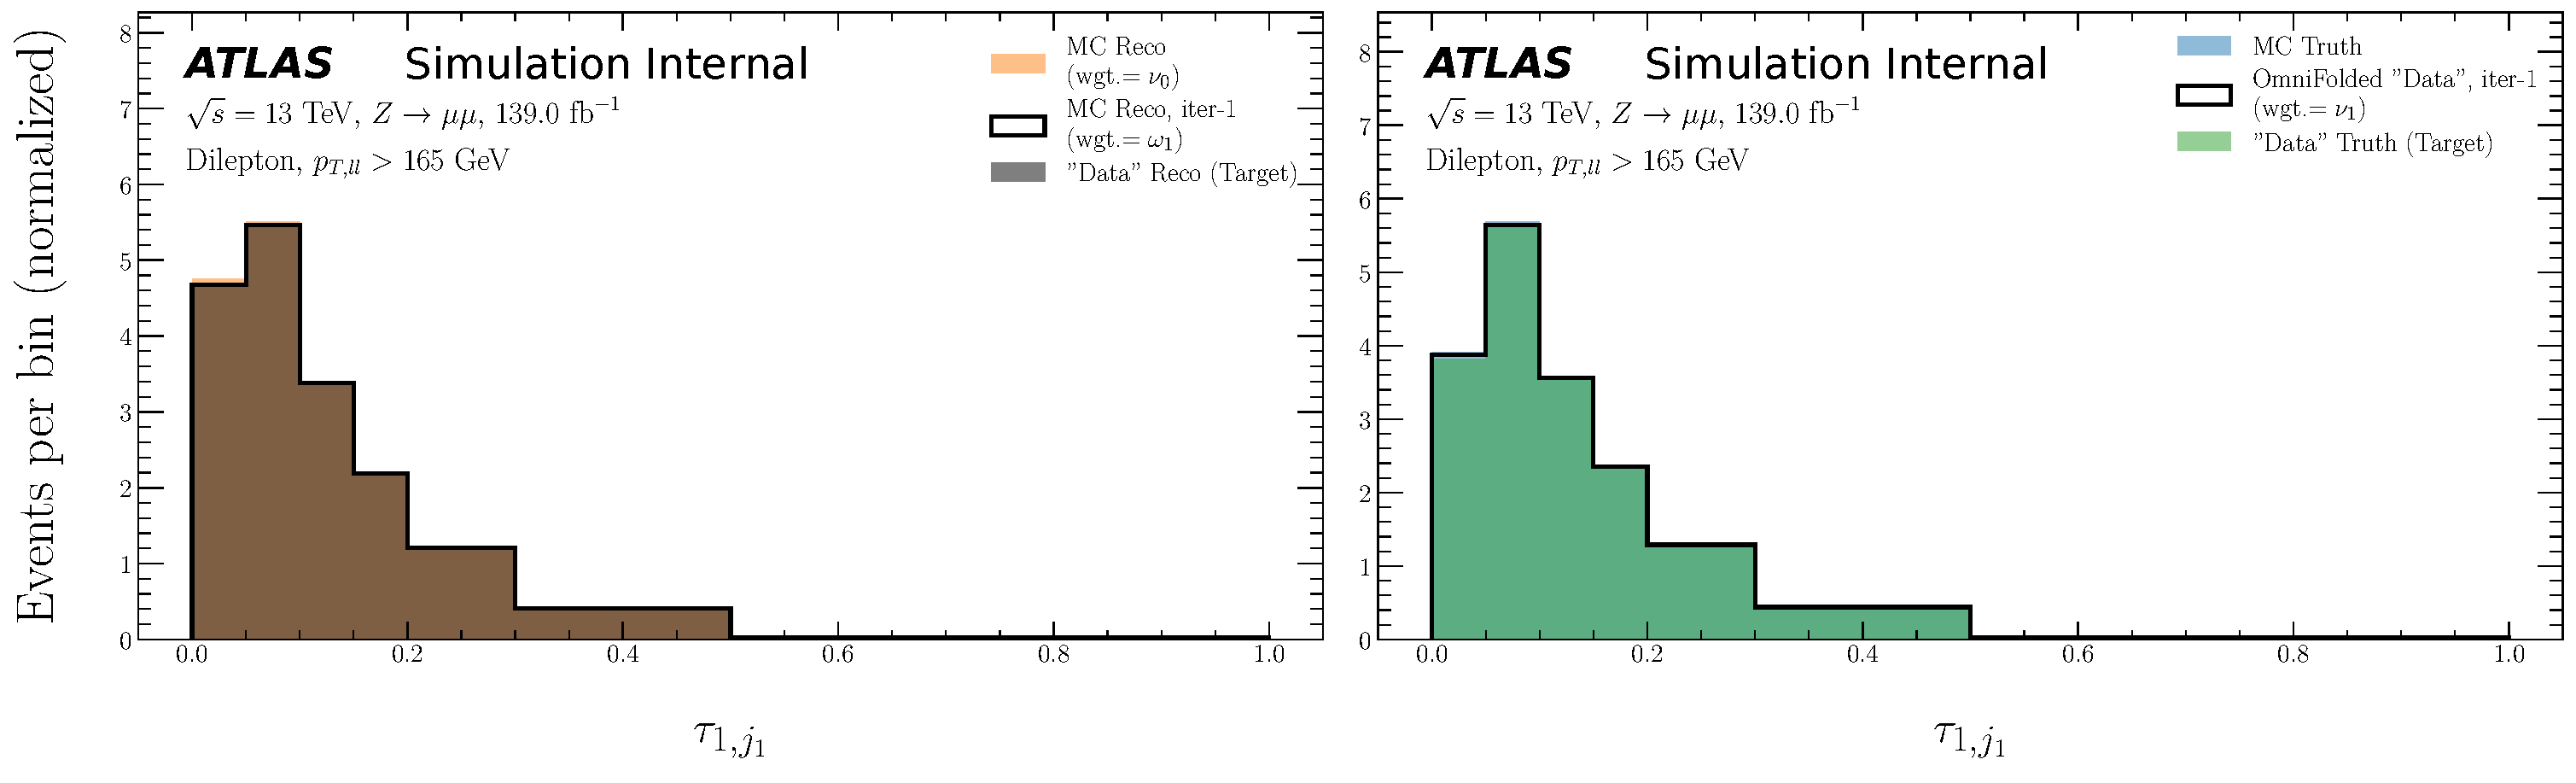
\includegraphics[width=0.85\textwidth]{figures/ATLASOmniFold-StressTest/ATLASOmniFold-StressTestA/UniFold/tau1_trackj1/ATLASOmniFold-StressTestA-UniFold-tau1_trackj1-Iteration01}}\\
\subfloat[After 2 iterations]{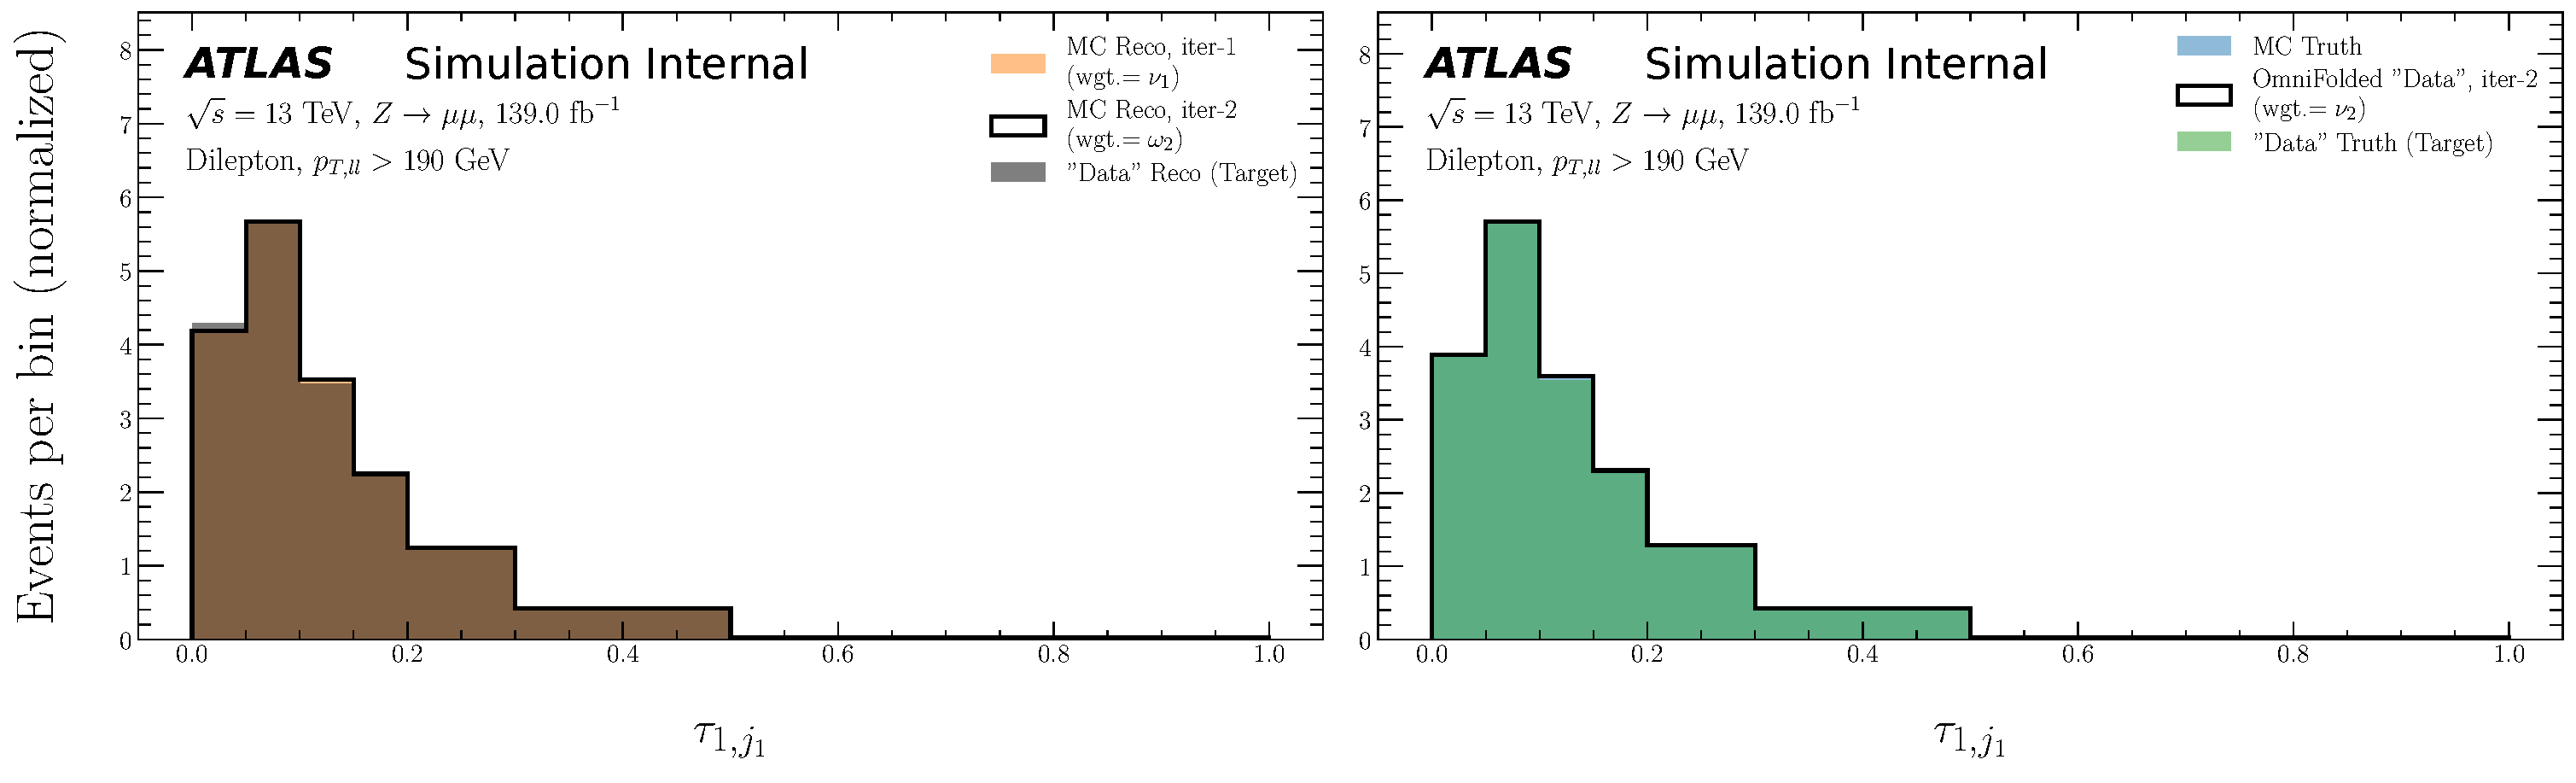
\includegraphics[width=0.85\textwidth]{figures/ATLASOmniFold-StressTest/ATLASOmniFold-StressTestA/UniFold/tau1_trackj1/ATLASOmniFold-StressTestA-UniFold-tau1_trackj1-Iteration02}}
\phantomcaption 
\end{figure}

\begin{figure}[h!]
\centering
\ContinuedFloat
\subfloat[After 3 iterations]{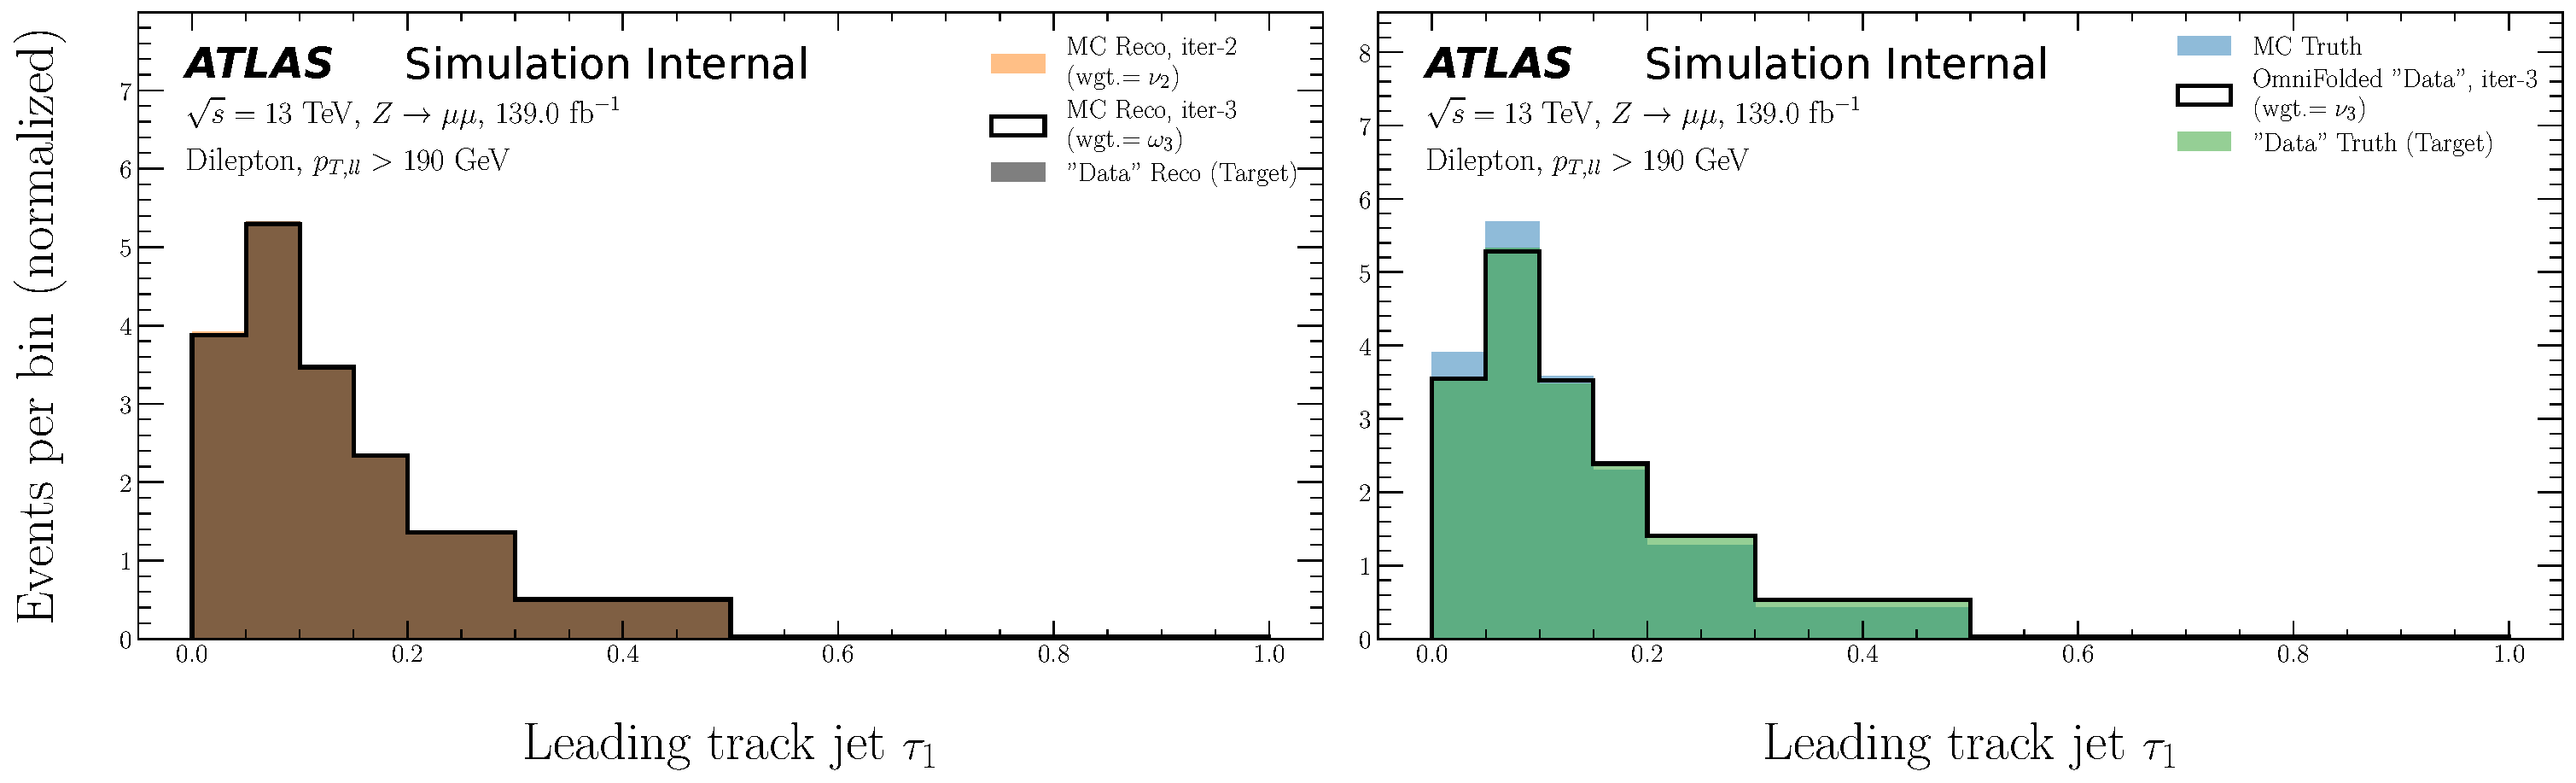
\includegraphics[width=0.85\textwidth]{figures/ATLASOmniFold-StressTest/ATLASOmniFold-StressTestA/UniFold/tau1_trackj1/ATLASOmniFold-StressTestA-UniFold-tau1_trackj1-Iteration03}}\\
\subfloat[After 4 iterations]{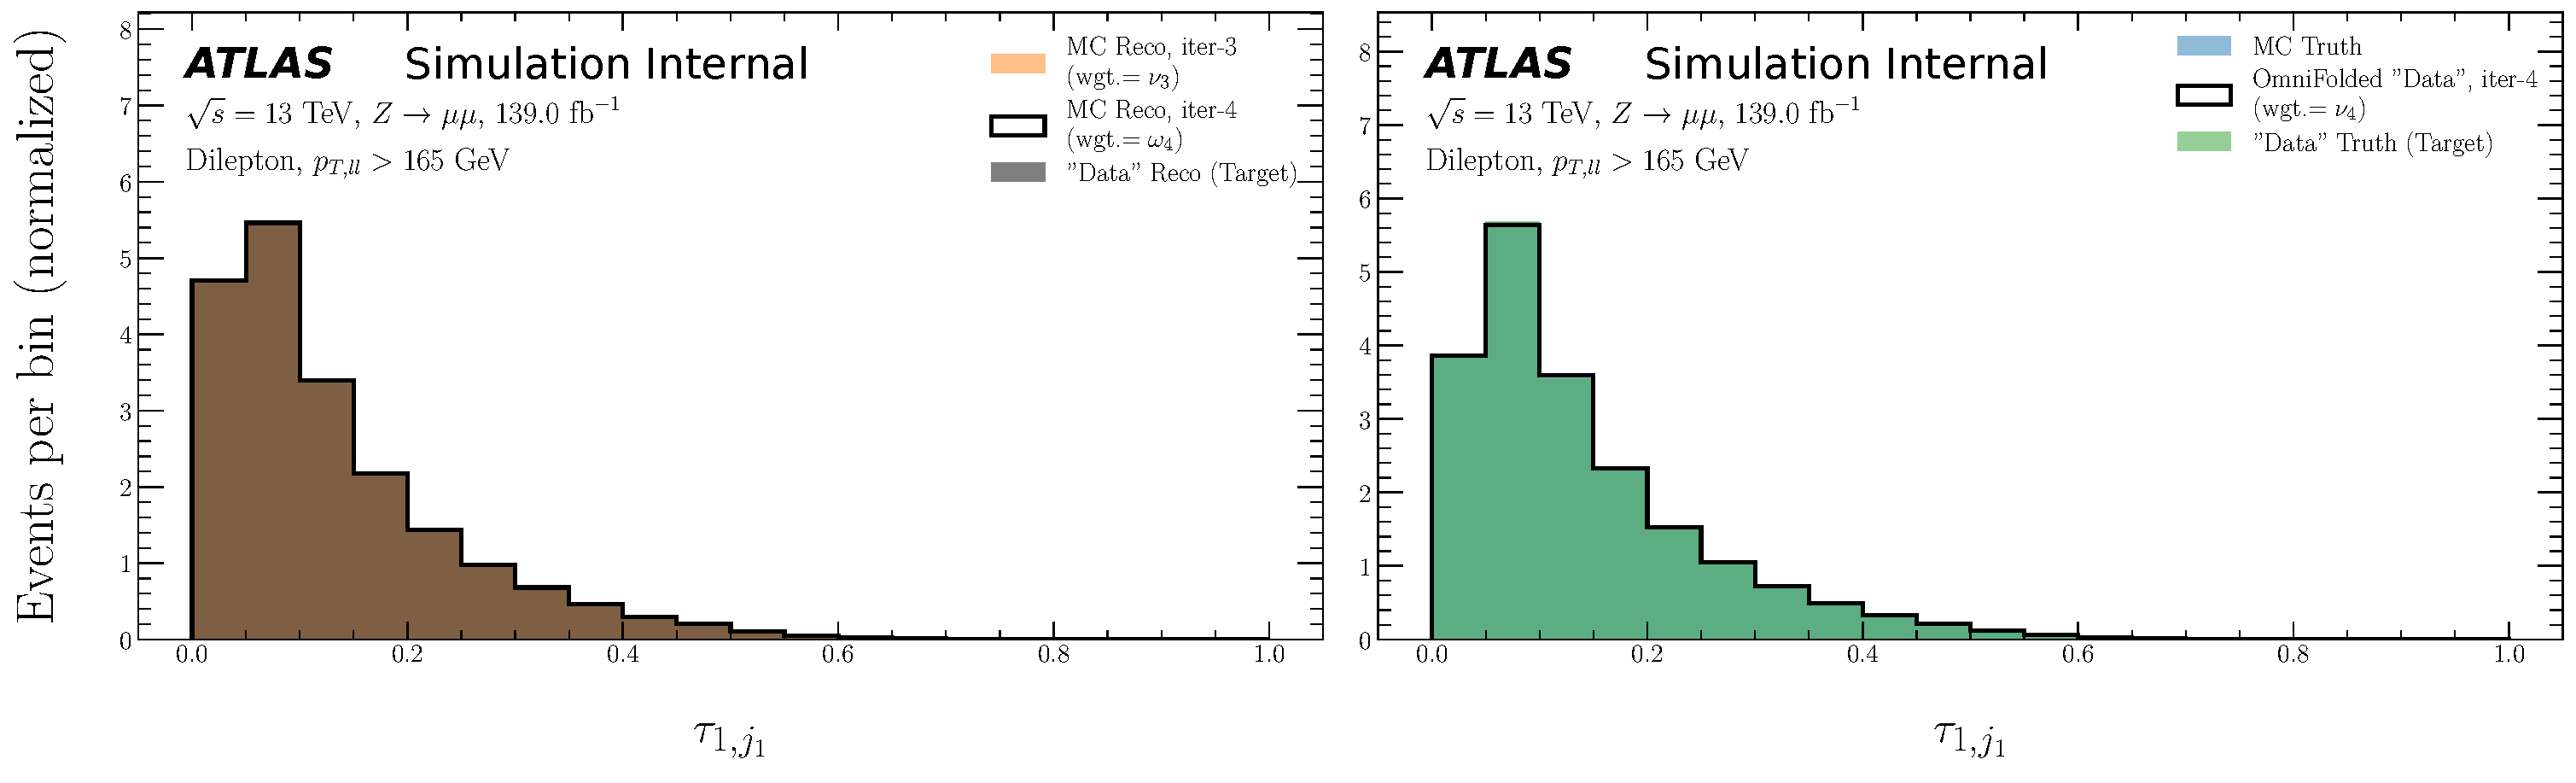
\includegraphics[width=0.85\textwidth]{figures/ATLASOmniFold-StressTest/ATLASOmniFold-StressTestA/UniFold/tau1_trackj1/ATLASOmniFold-StressTestA-UniFold-tau1_trackj1-Iteration04}}\\
\subfloat[After 5 iterations]{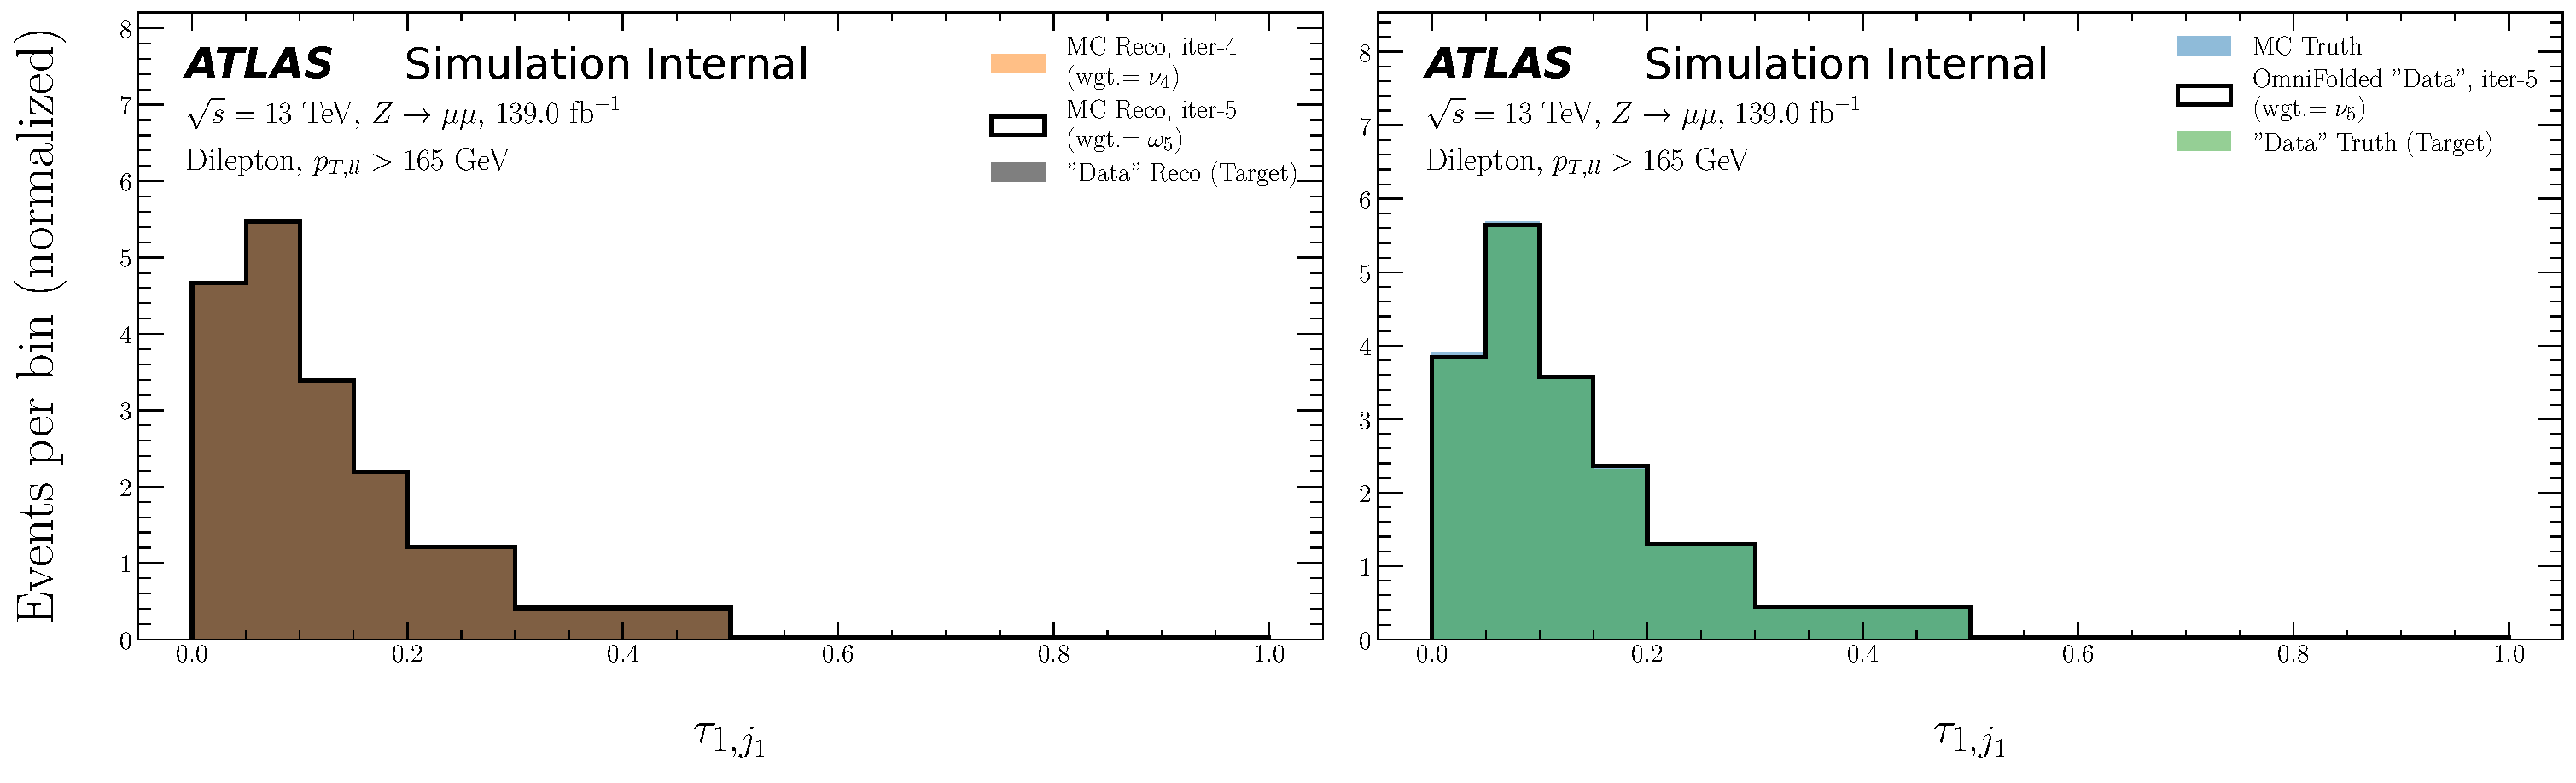
\includegraphics[width=0.85\textwidth]{figures/ATLASOmniFold-StressTest/ATLASOmniFold-StressTestA/UniFold/tau1_trackj1/ATLASOmniFold-StressTestA-UniFold-tau1_trackj1-Iteration05}}\\
\subfloat[After 6 iterations]{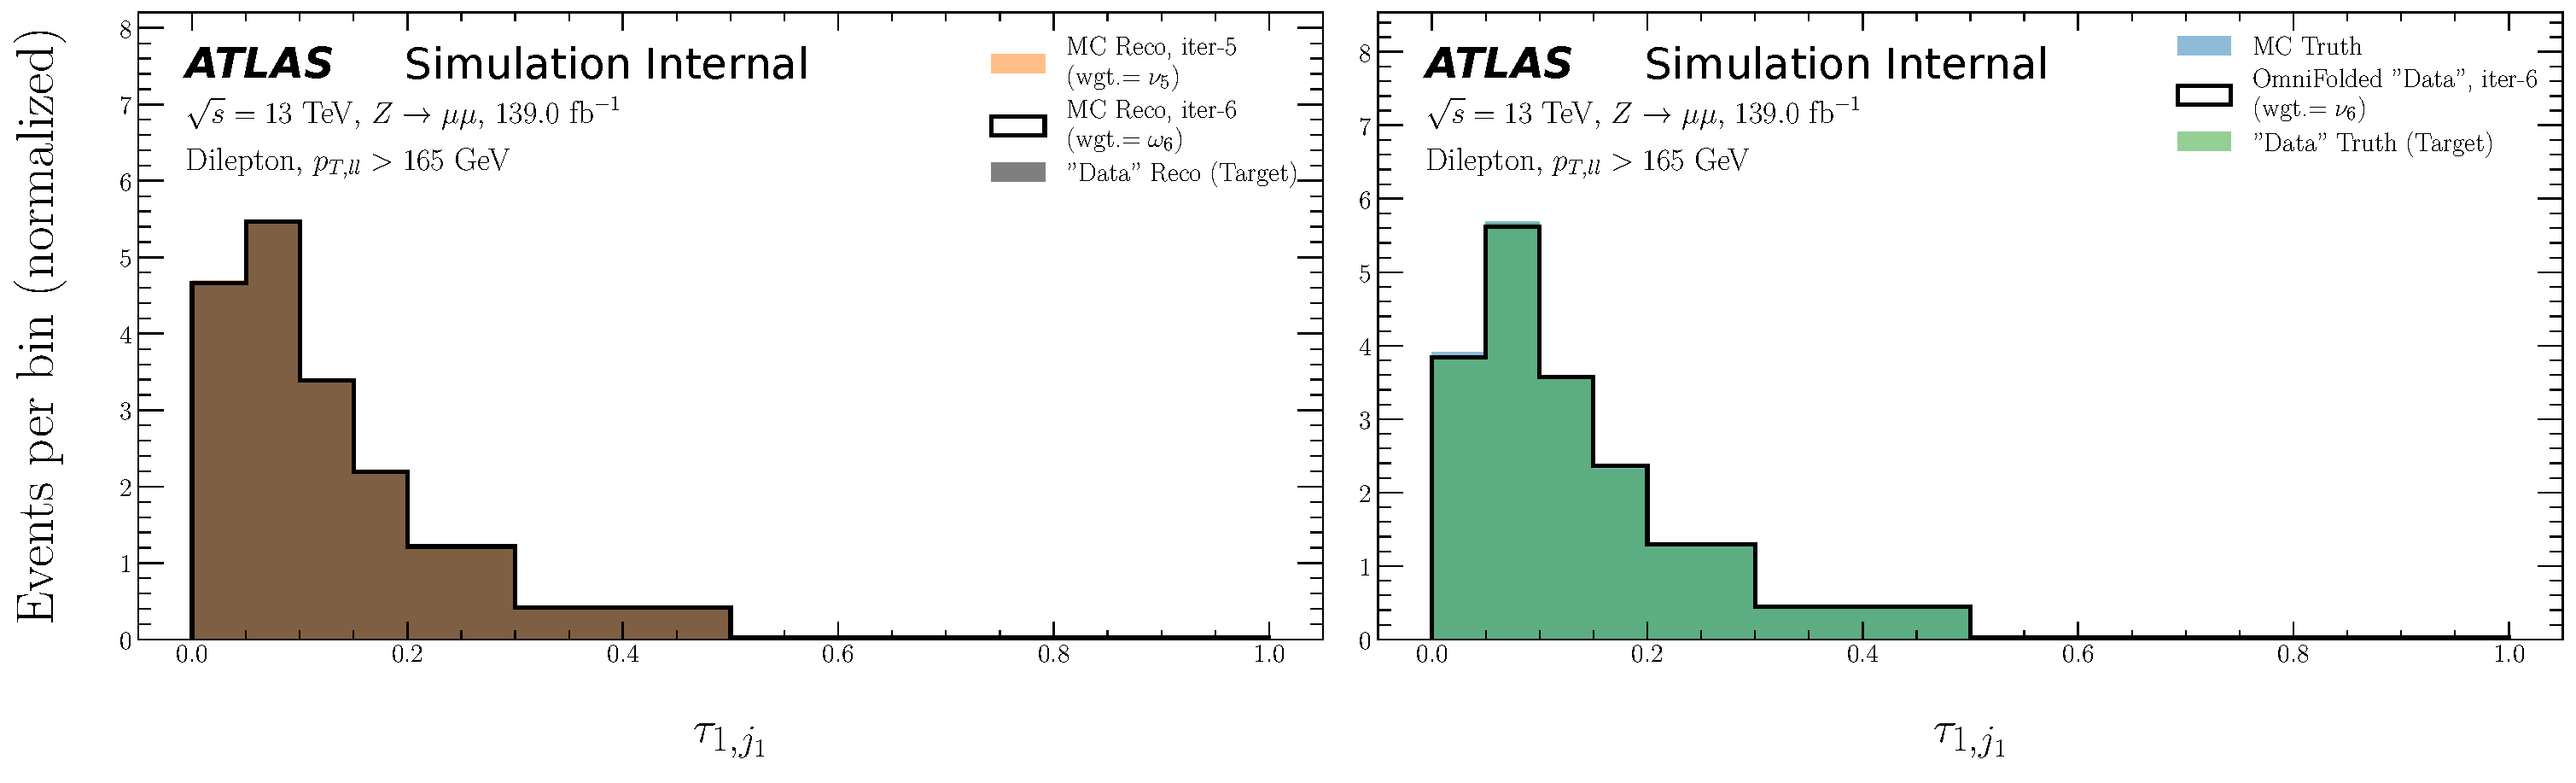
\includegraphics[width=0.85\textwidth]{figures/ATLASOmniFold-StressTest/ATLASOmniFold-StressTestA/UniFold/tau1_trackj1/ATLASOmniFold-StressTestA-UniFold-tau1_trackj1-Iteration06}}
\caption{A stress test for UniFold applied to the leading track jet $\tau_1$.}
\label{fig:stressa_tau1_trackj1}
\end{figure}

\begin{figure}[h!]
\centering
\subfloat[Weights]{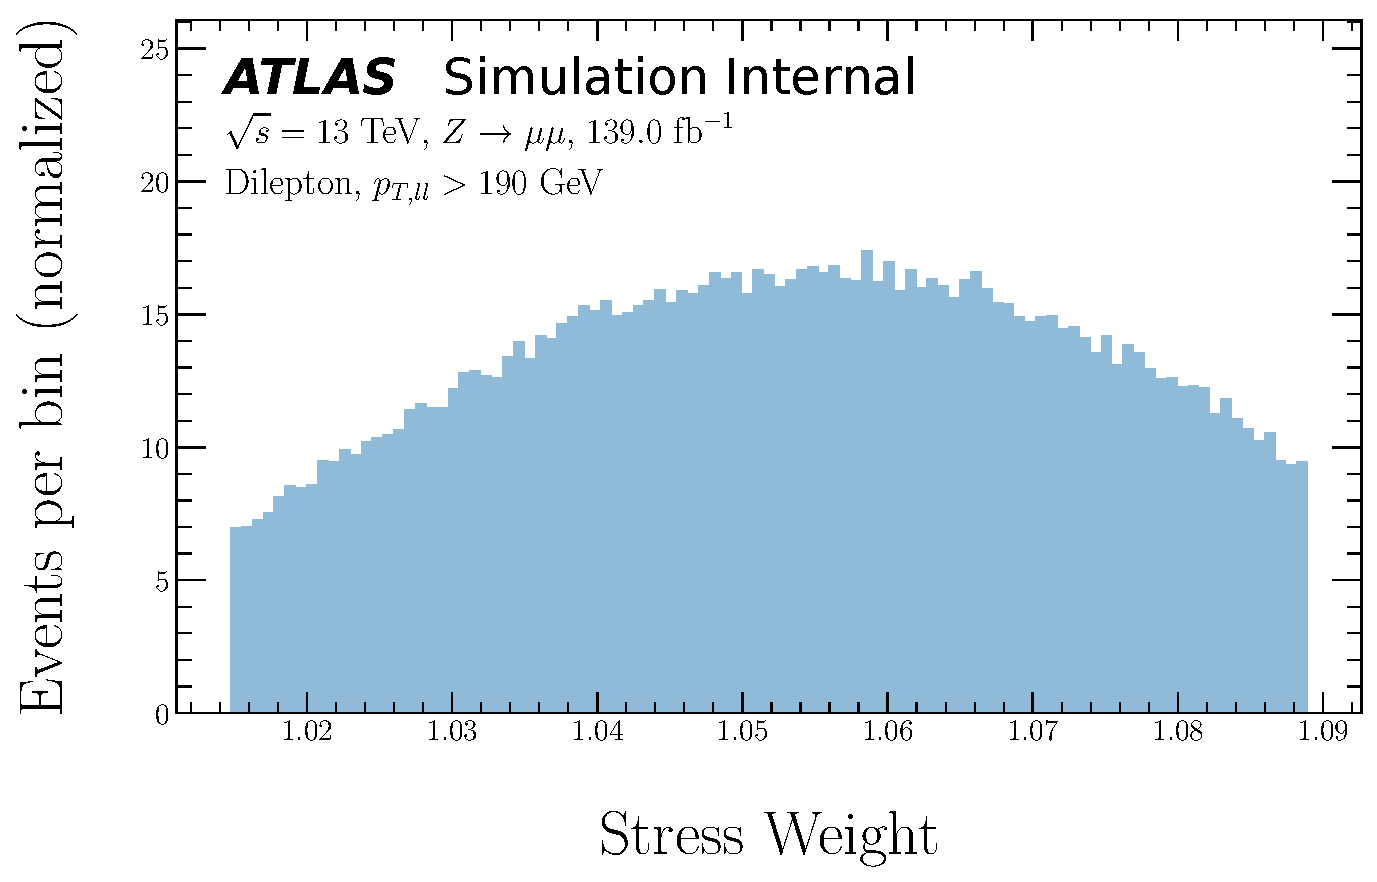
\includegraphics[width=0.45\textwidth]{figures/ATLASOmniFold-StressTest/ATLASOmniFold-StressTestA/UniFold/y_trackj1/ATLASOmniFold-StressTestA-UniFold-y_trackj1-StressWeightsHist.pdf}}\\
\subfloat[Input histograms]{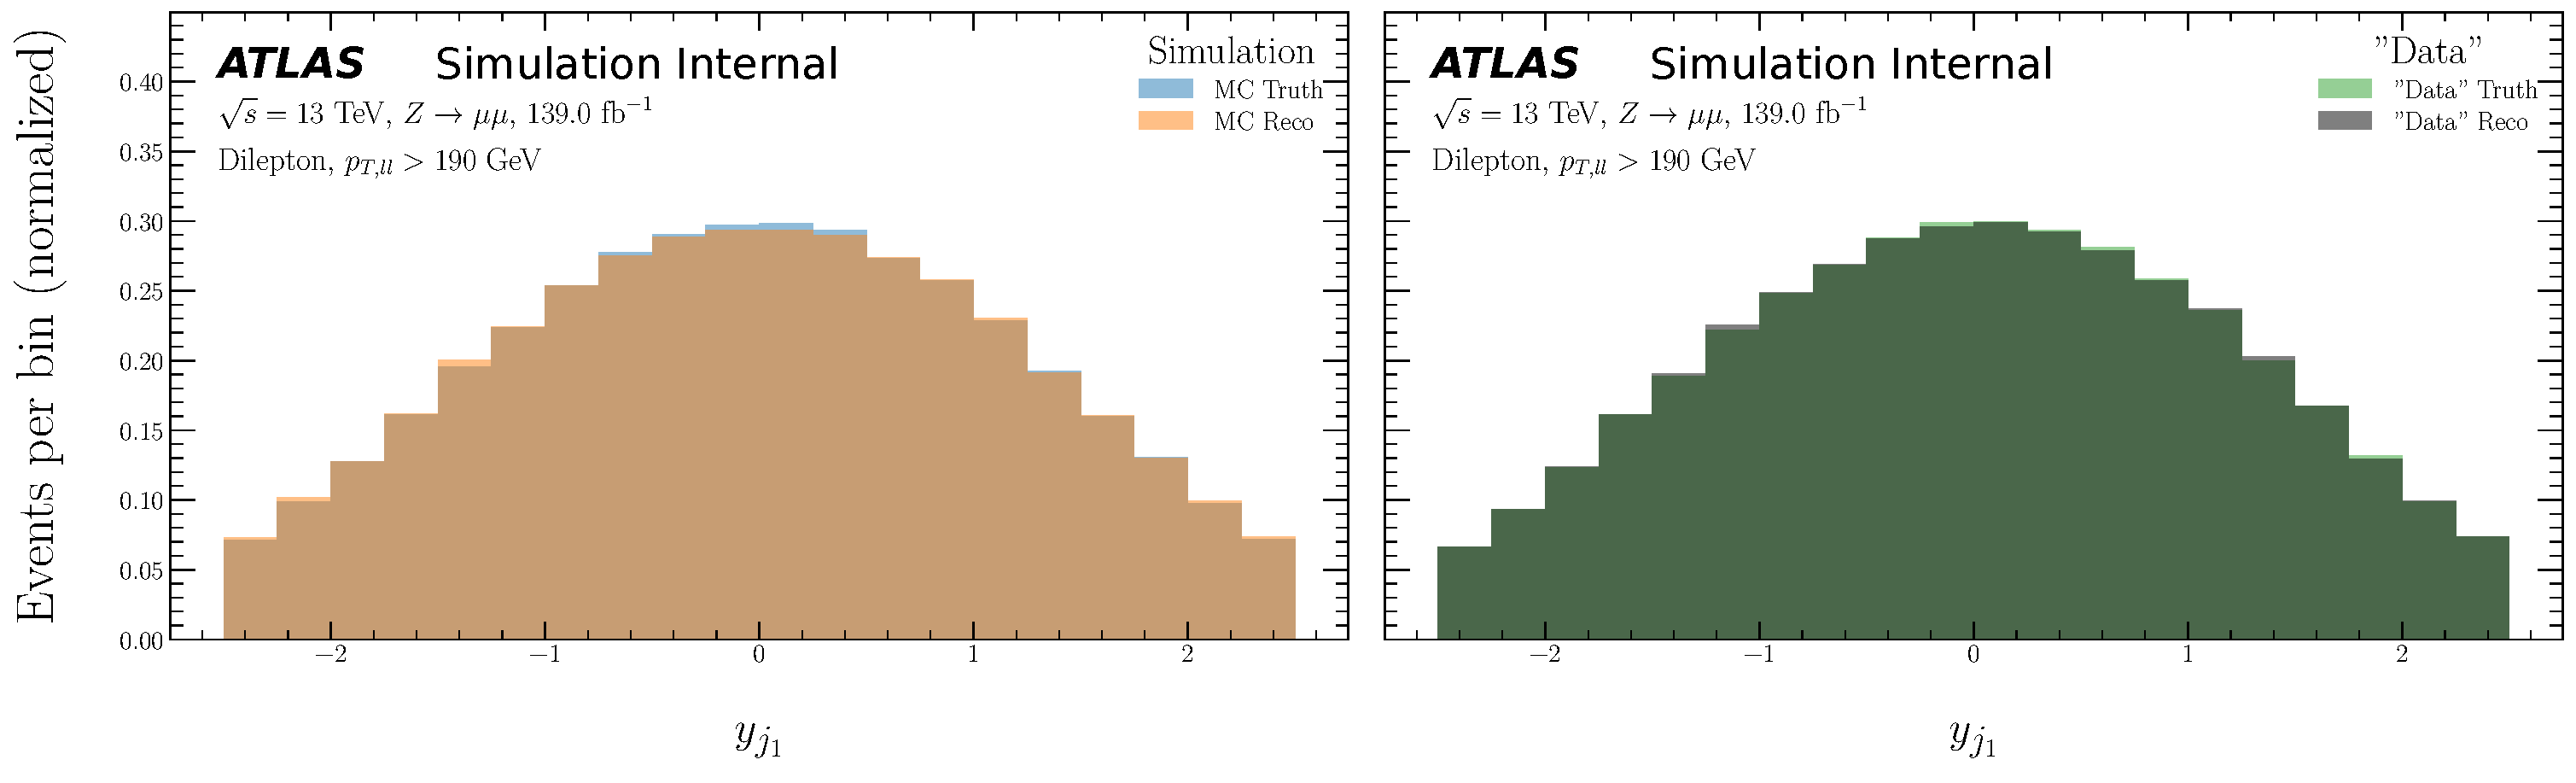
\includegraphics[width=0.85\textwidth]{figures/ATLASOmniFold-StressTest/ATLASOmniFold-StressTestA/UniFold/y_trackj1/ATLASOmniFold-StressTestA-UniFold-y_trackj1-Distributions}}\\
\subfloat[After 1 iteration]{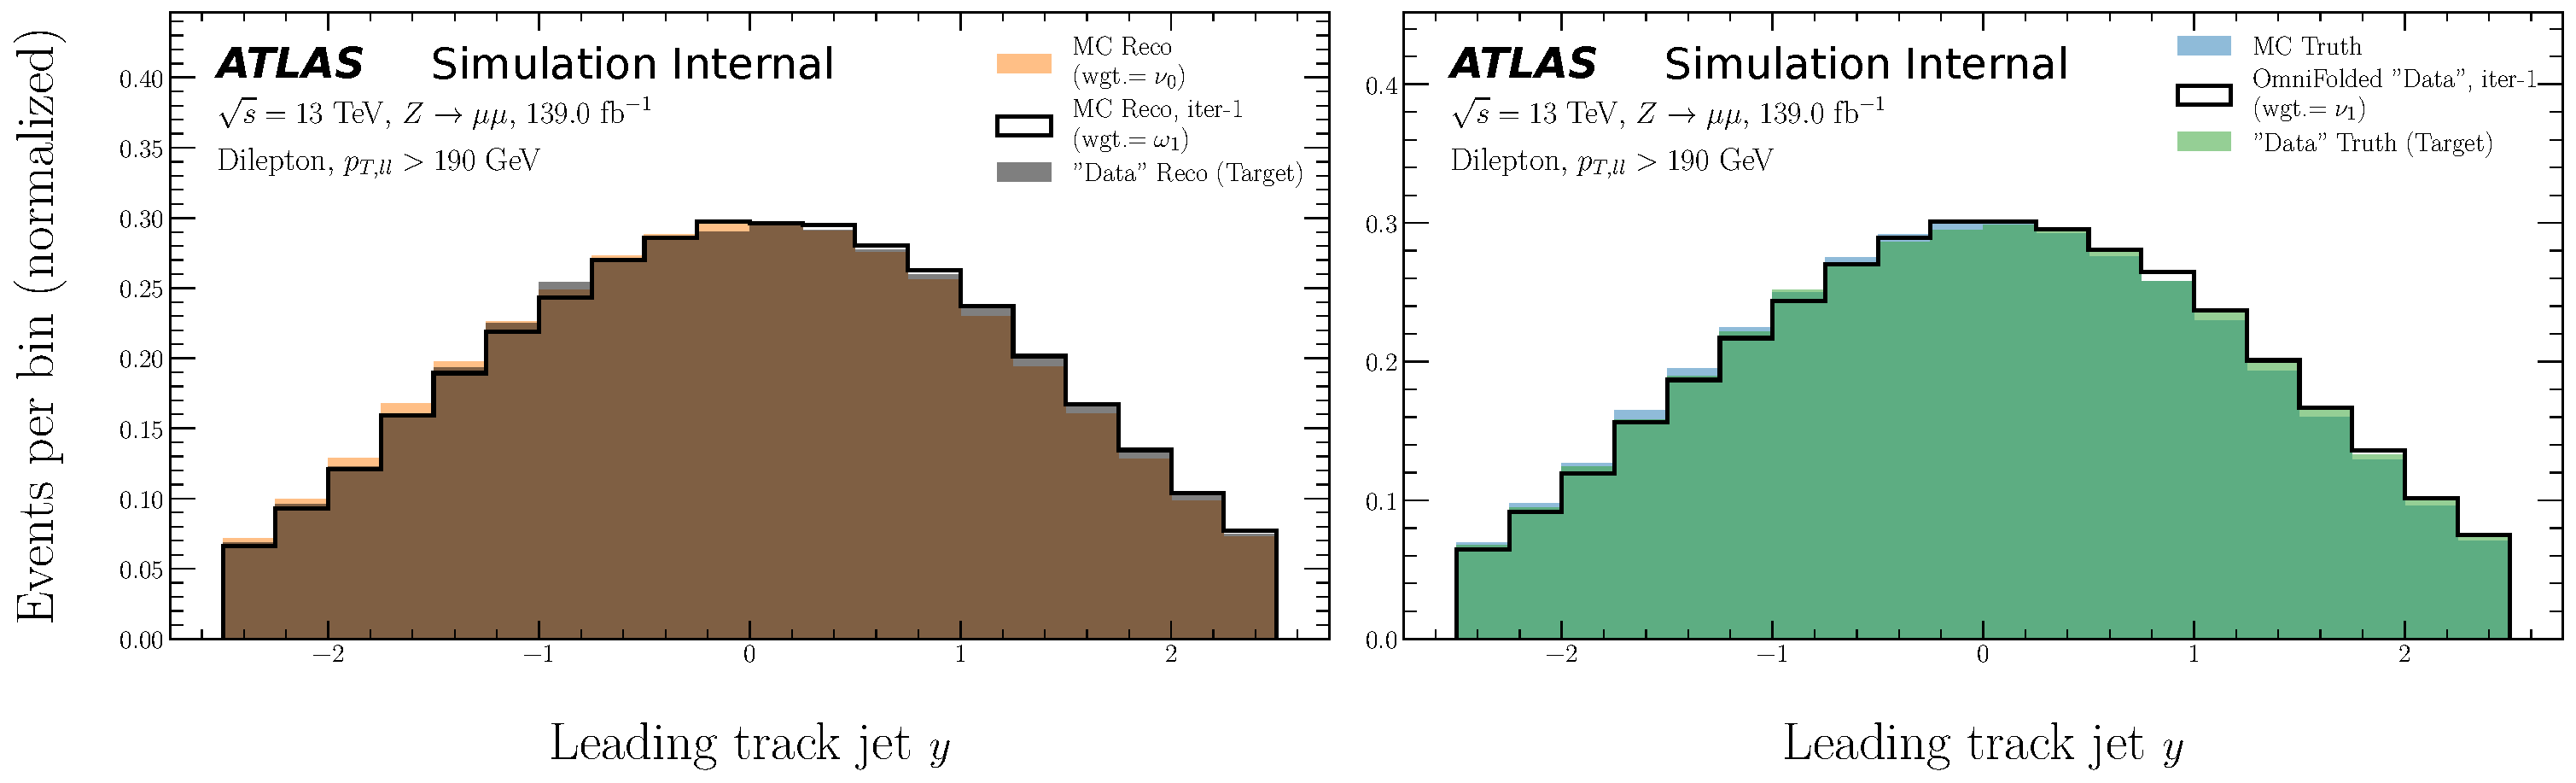
\includegraphics[width=0.85\textwidth]{figures/ATLASOmniFold-StressTest/ATLASOmniFold-StressTestA/UniFold/y_trackj1/ATLASOmniFold-StressTestA-UniFold-y_trackj1-Iteration01}}\\
\subfloat[After 2 iterations]{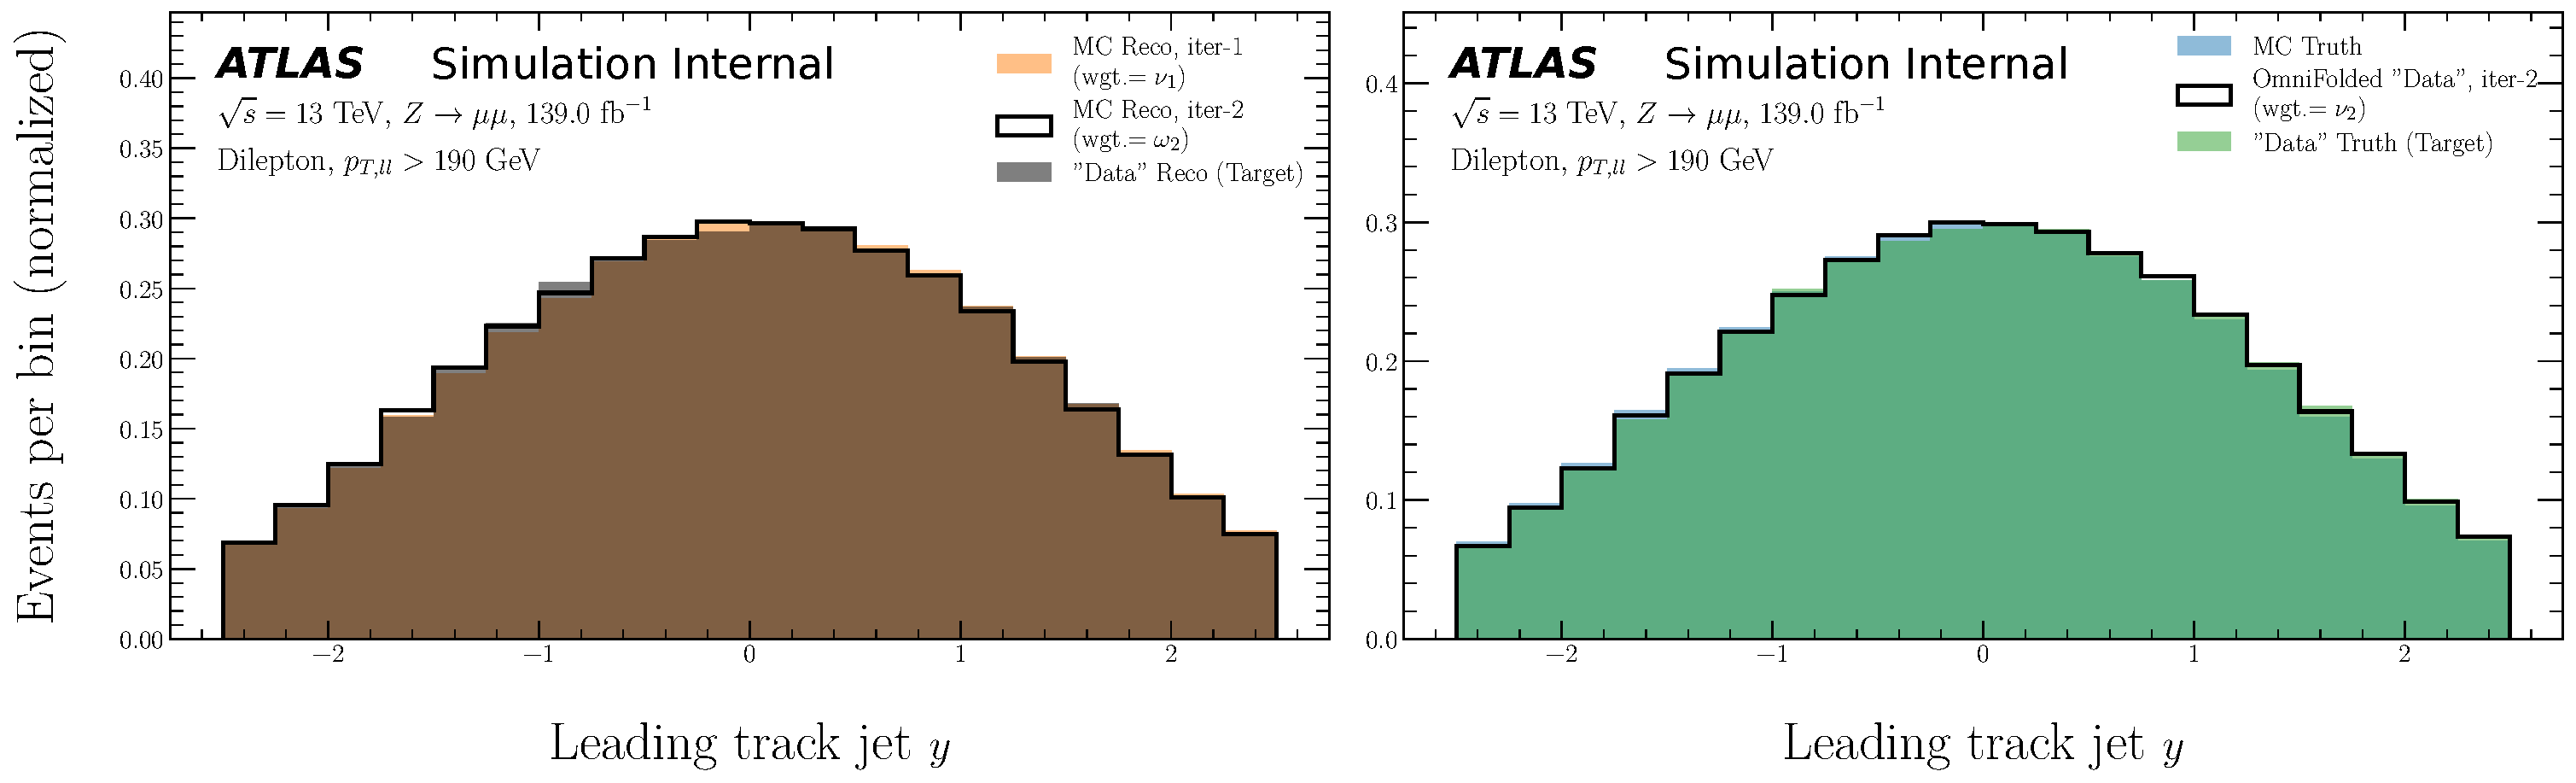
\includegraphics[width=0.85\textwidth]{figures/ATLASOmniFold-StressTest/ATLASOmniFold-StressTestA/UniFold/y_trackj1/ATLASOmniFold-StressTestA-UniFold-y_trackj1-Iteration02}}
\phantomcaption 
\end{figure}

\begin{figure}[h!]
\centering
\ContinuedFloat
\subfloat[After 3 iterations]{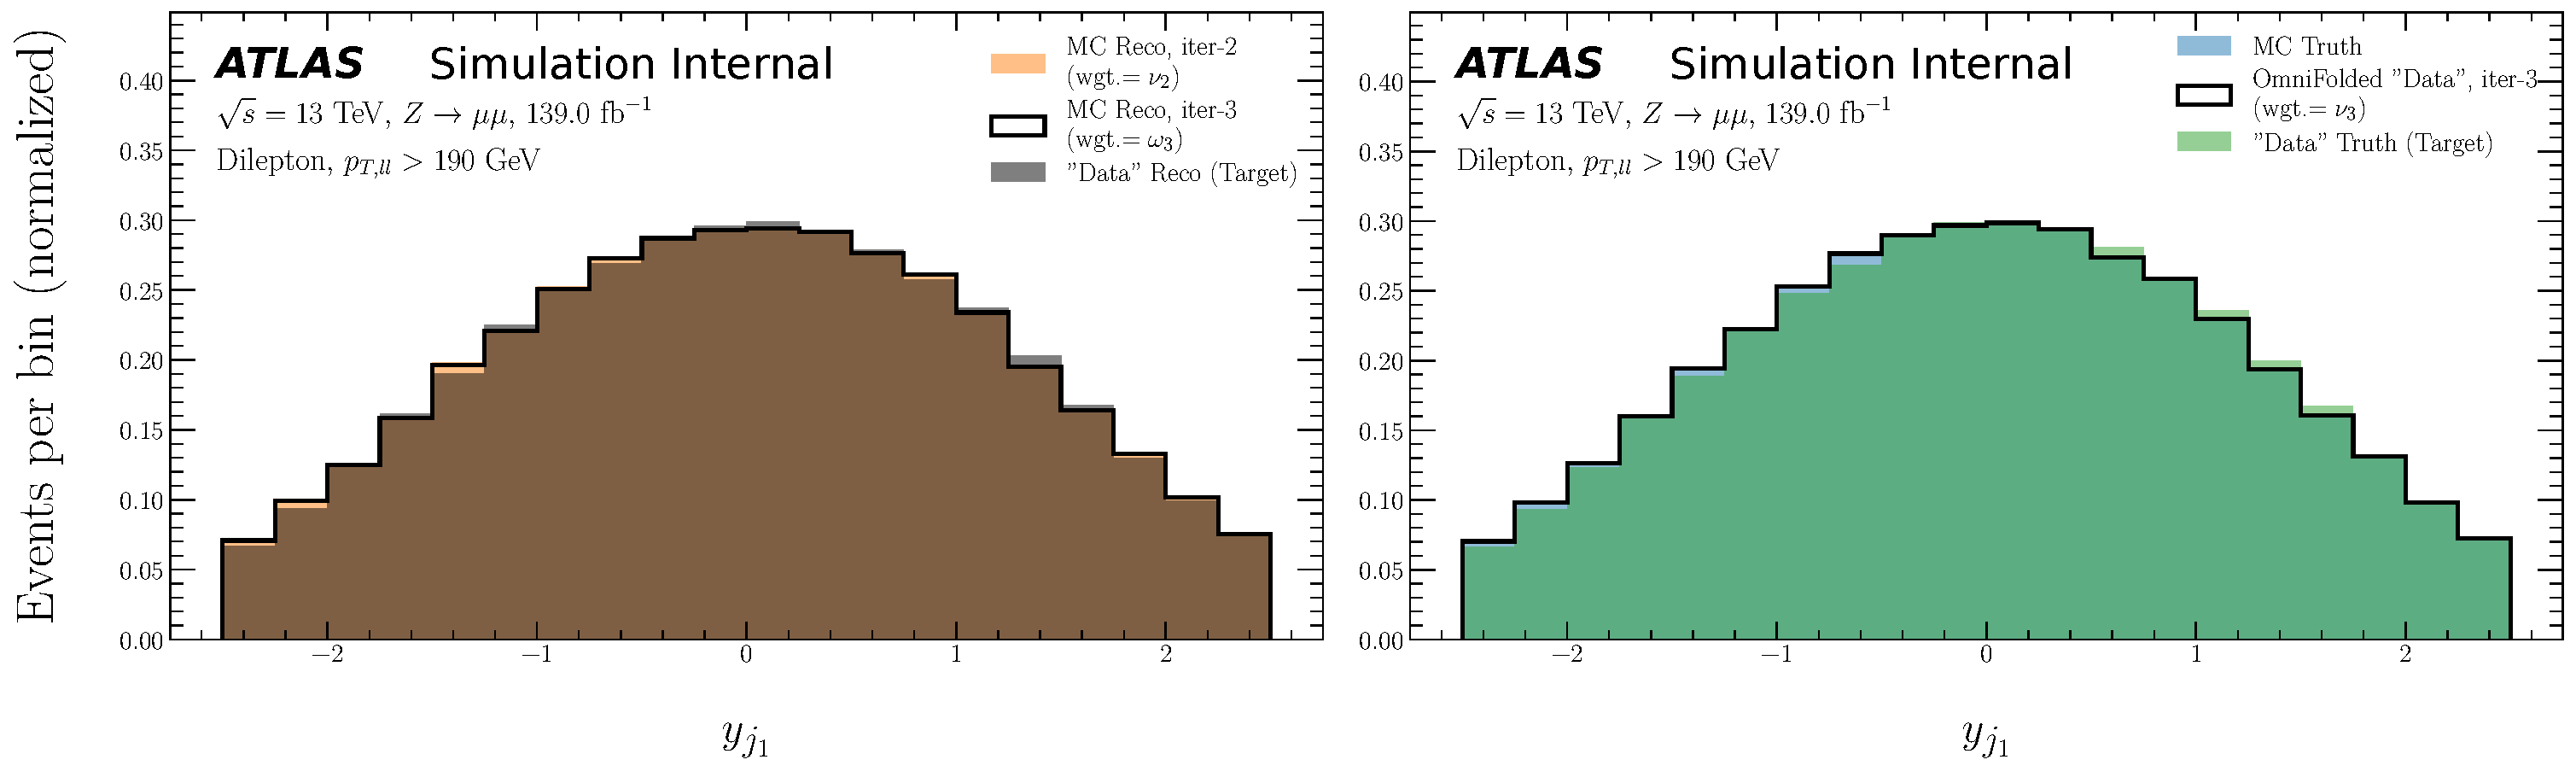
\includegraphics[width=0.85\textwidth]{figures/ATLASOmniFold-StressTest/ATLASOmniFold-StressTestA/UniFold/y_trackj1/ATLASOmniFold-StressTestA-UniFold-y_trackj1-Iteration03}}\\
\subfloat[After 4 iterations]{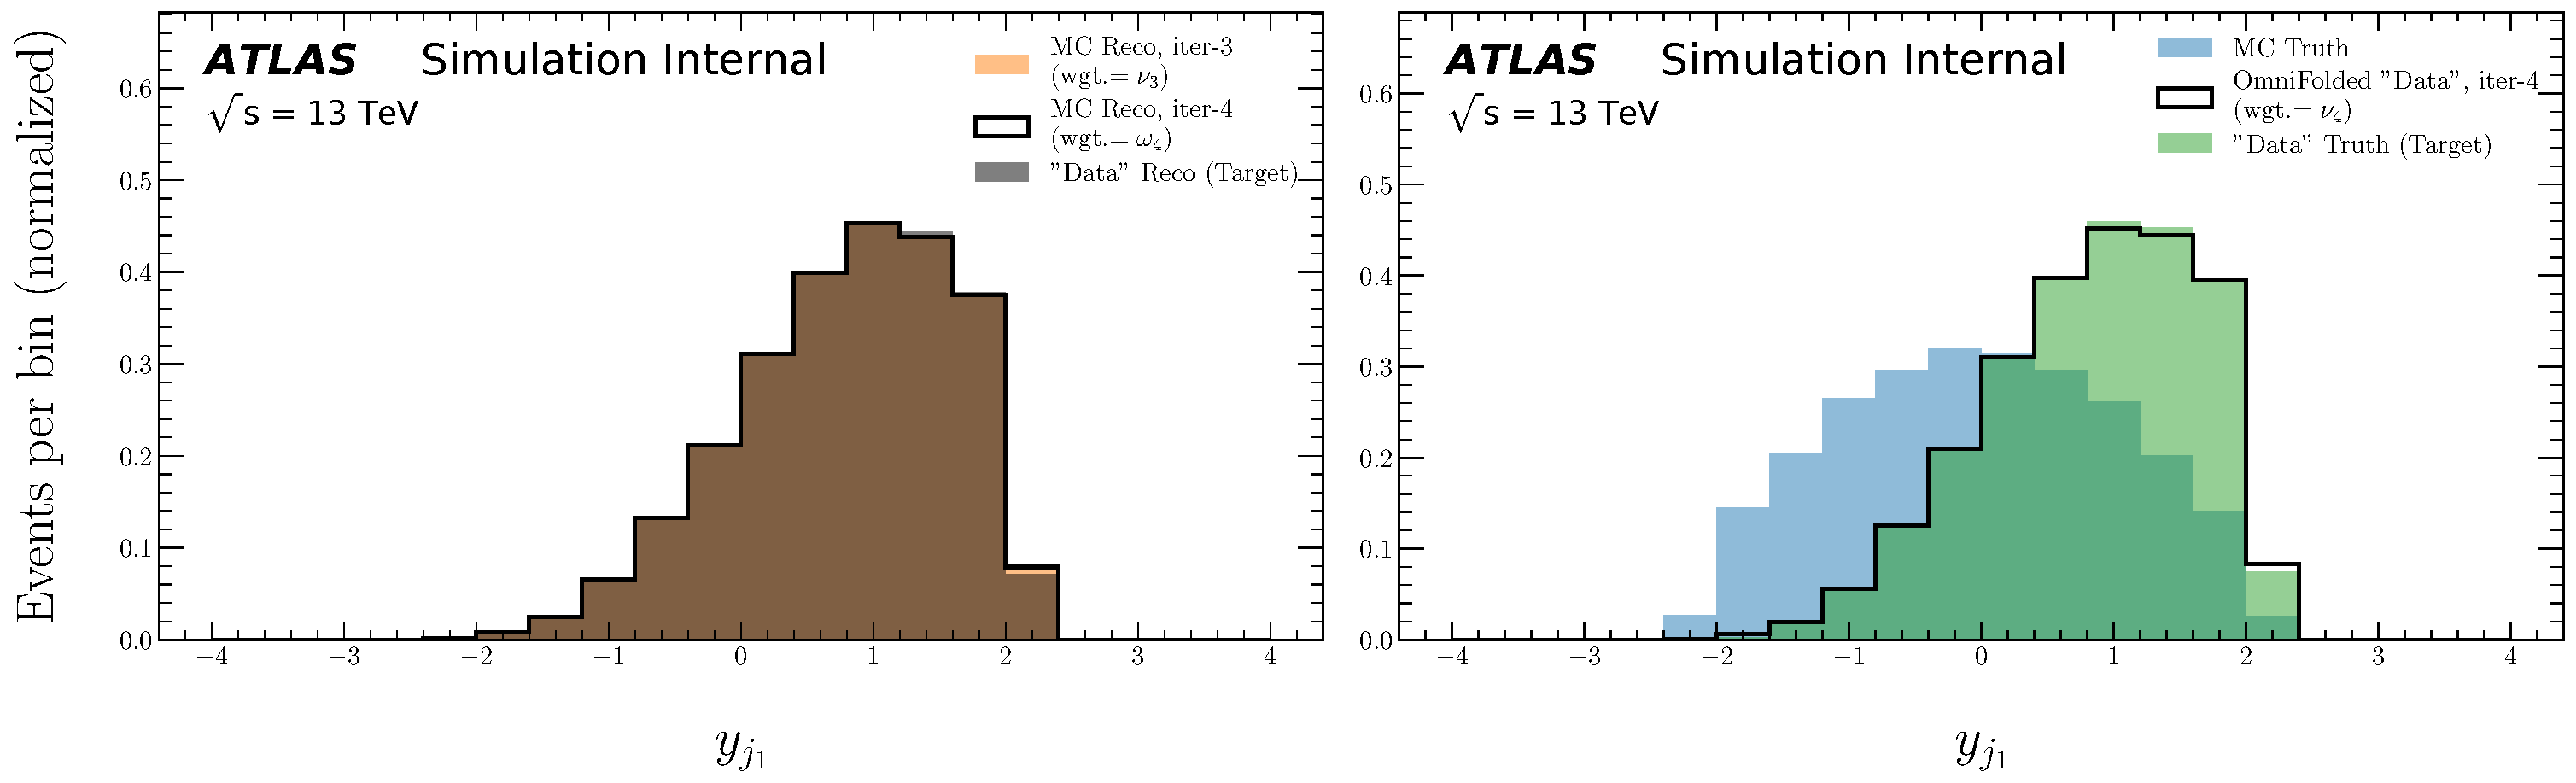
\includegraphics[width=0.85\textwidth]{figures/ATLASOmniFold-StressTest/ATLASOmniFold-StressTestA/UniFold/y_trackj1/ATLASOmniFold-StressTestA-UniFold-y_trackj1-Iteration04}}\\
\subfloat[After 5 iterations]{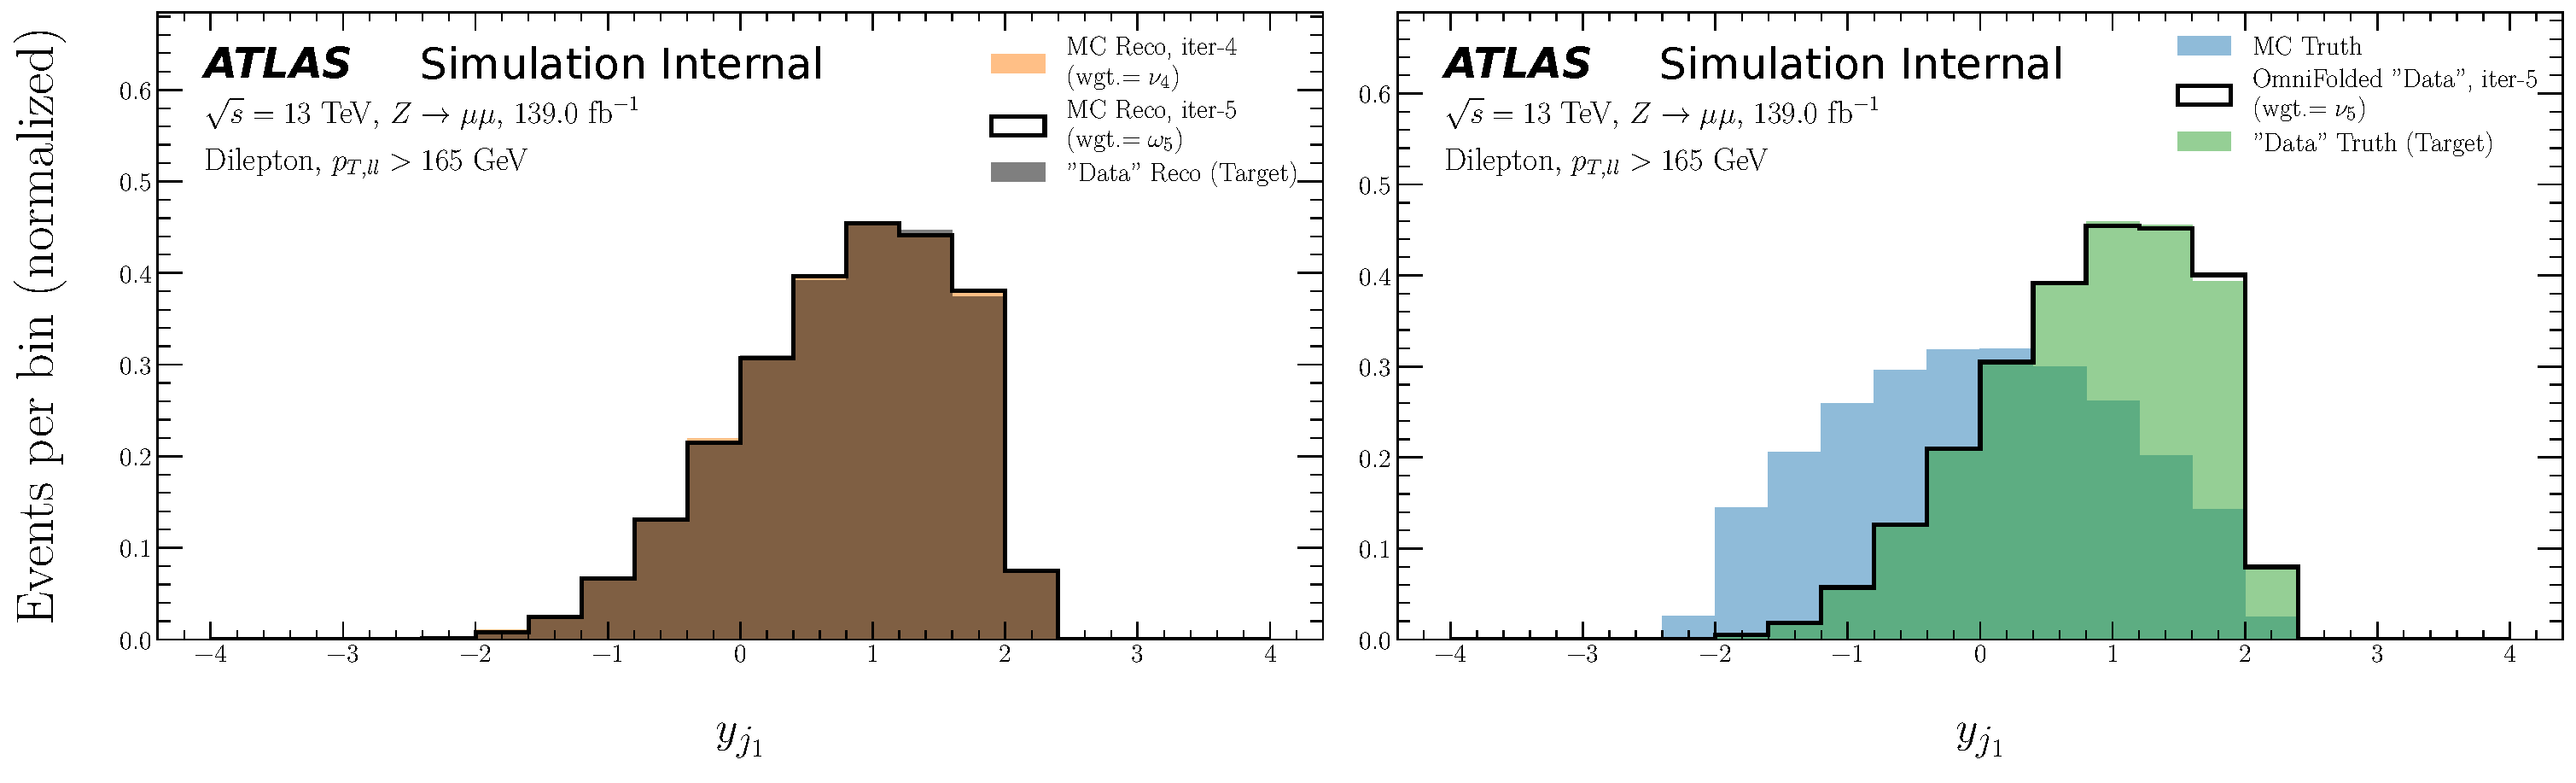
\includegraphics[width=0.85\textwidth]{figures/ATLASOmniFold-StressTest/ATLASOmniFold-StressTestA/UniFold/y_trackj1/ATLASOmniFold-StressTestA-UniFold-y_trackj1-Iteration05}}\\
\subfloat[After 6 iterations]{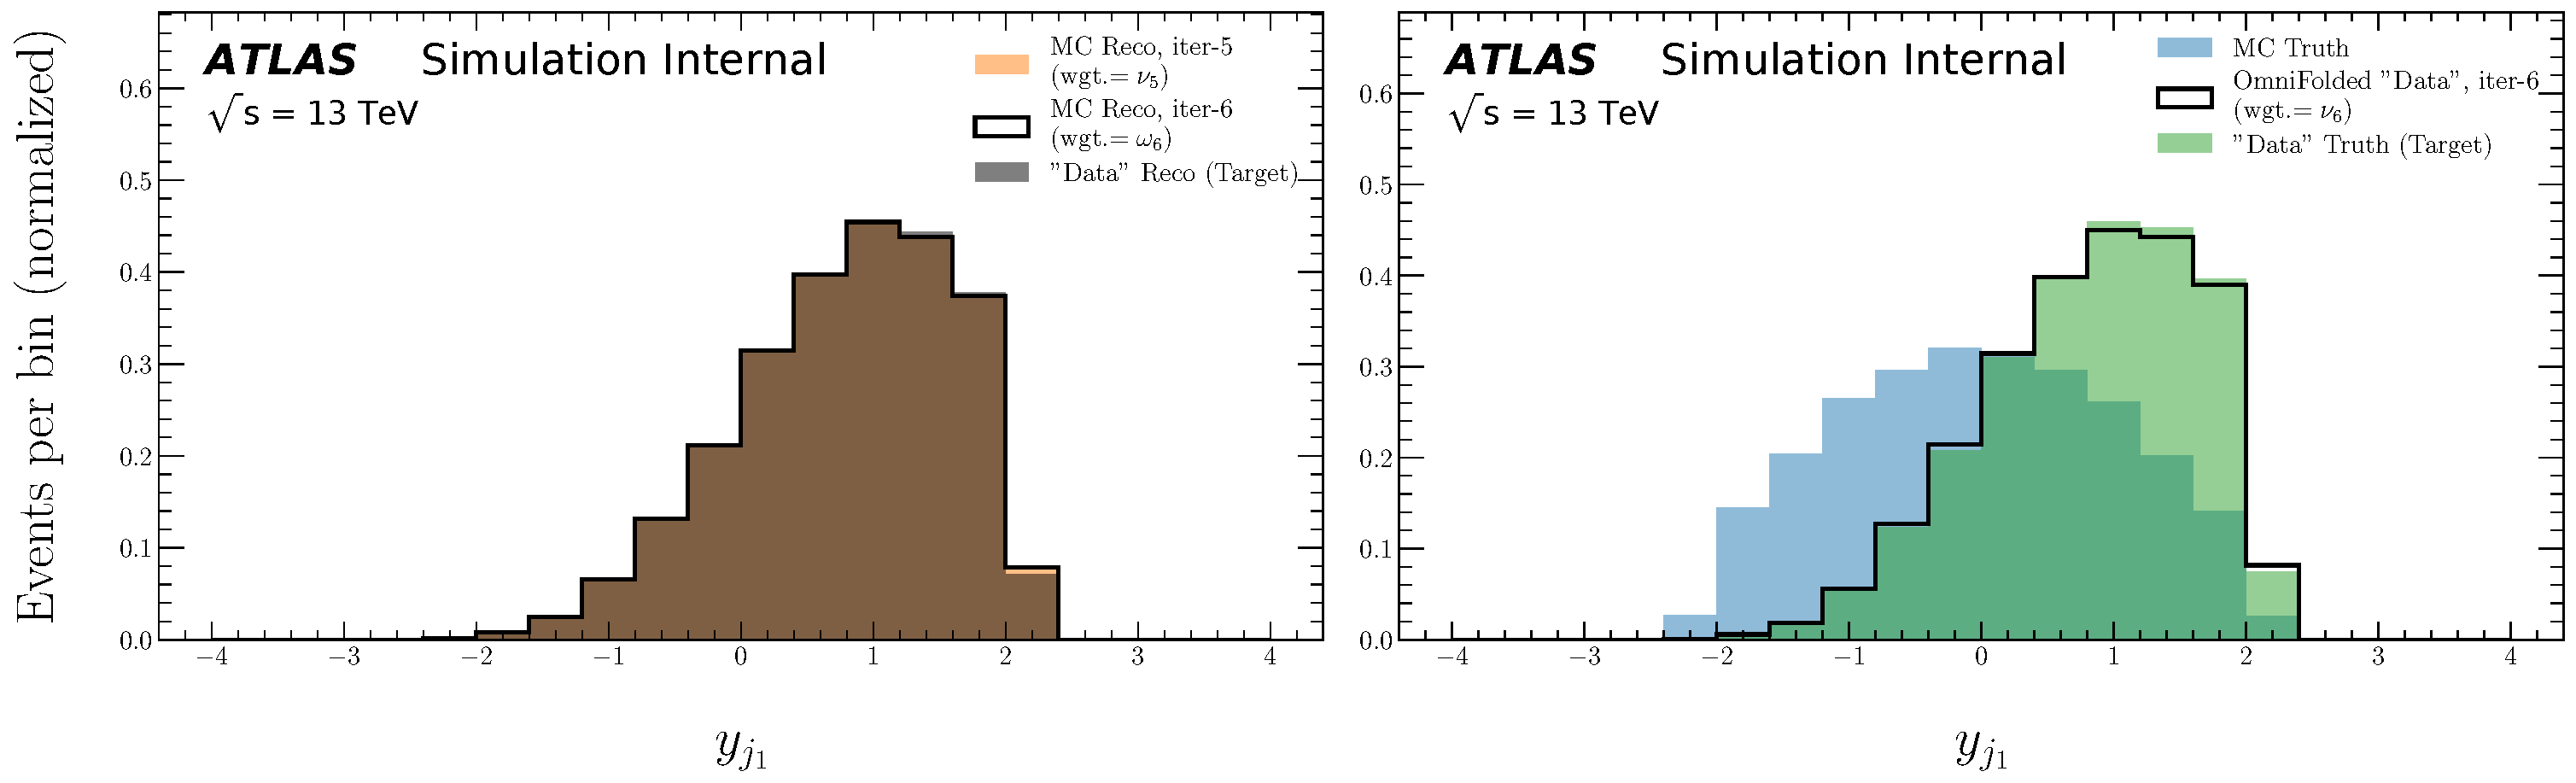
\includegraphics[width=0.85\textwidth]{figures/ATLASOmniFold-StressTest/ATLASOmniFold-StressTestA/UniFold/y_trackj1/ATLASOmniFold-StressTestA-UniFold-y_trackj1-Iteration06}}
\caption{A stress test for UniFold applied to the leading track jet rapidity.}
\label{fig:stressa_y_trackj1}
\end{figure}

\section{Deterministic Stress Tests for MultiFold}
\label{sec:stressmultifolddet}

Following from Sec.~\ref{sec:stress:deterministic}, Figures~\ref{fig:stressa_pT_trackj1Multi},~\ref{fig:stressa_y_trackj1Multi},~\ref{fig:stressa_tau1_trackj1Multi},~\ref{fig:stressa_tau2_trackj1Multi},~\ref{fig:stressa_tau3_trackj1Multi}, show the MultiFold results for the properties of the leading track jet, Figs.~\ref{fig:stressa_massMulti},~\ref{fig:stressa_Ntracks_trackj2Multi},~\ref{fig:stressa_pT_trackj2Multi},~\ref{fig:stressa_y_trackj2Multi},~\ref{fig:stressa_tau1_trackj2Multi},~\ref{fig:stressa_tau2_trackj2Multi},~\ref{fig:stressa_tau3_trackj2Multi} show the unfolded properties of the subleading track jet and Fig.~\ref{fig:stressa_pT_llMulti} and Fig.~\ref{fig:stressa_y_llMulti} for the dilepton properties.

\begin{figure}[h!]
\centering
\subfloat[Input histograms]{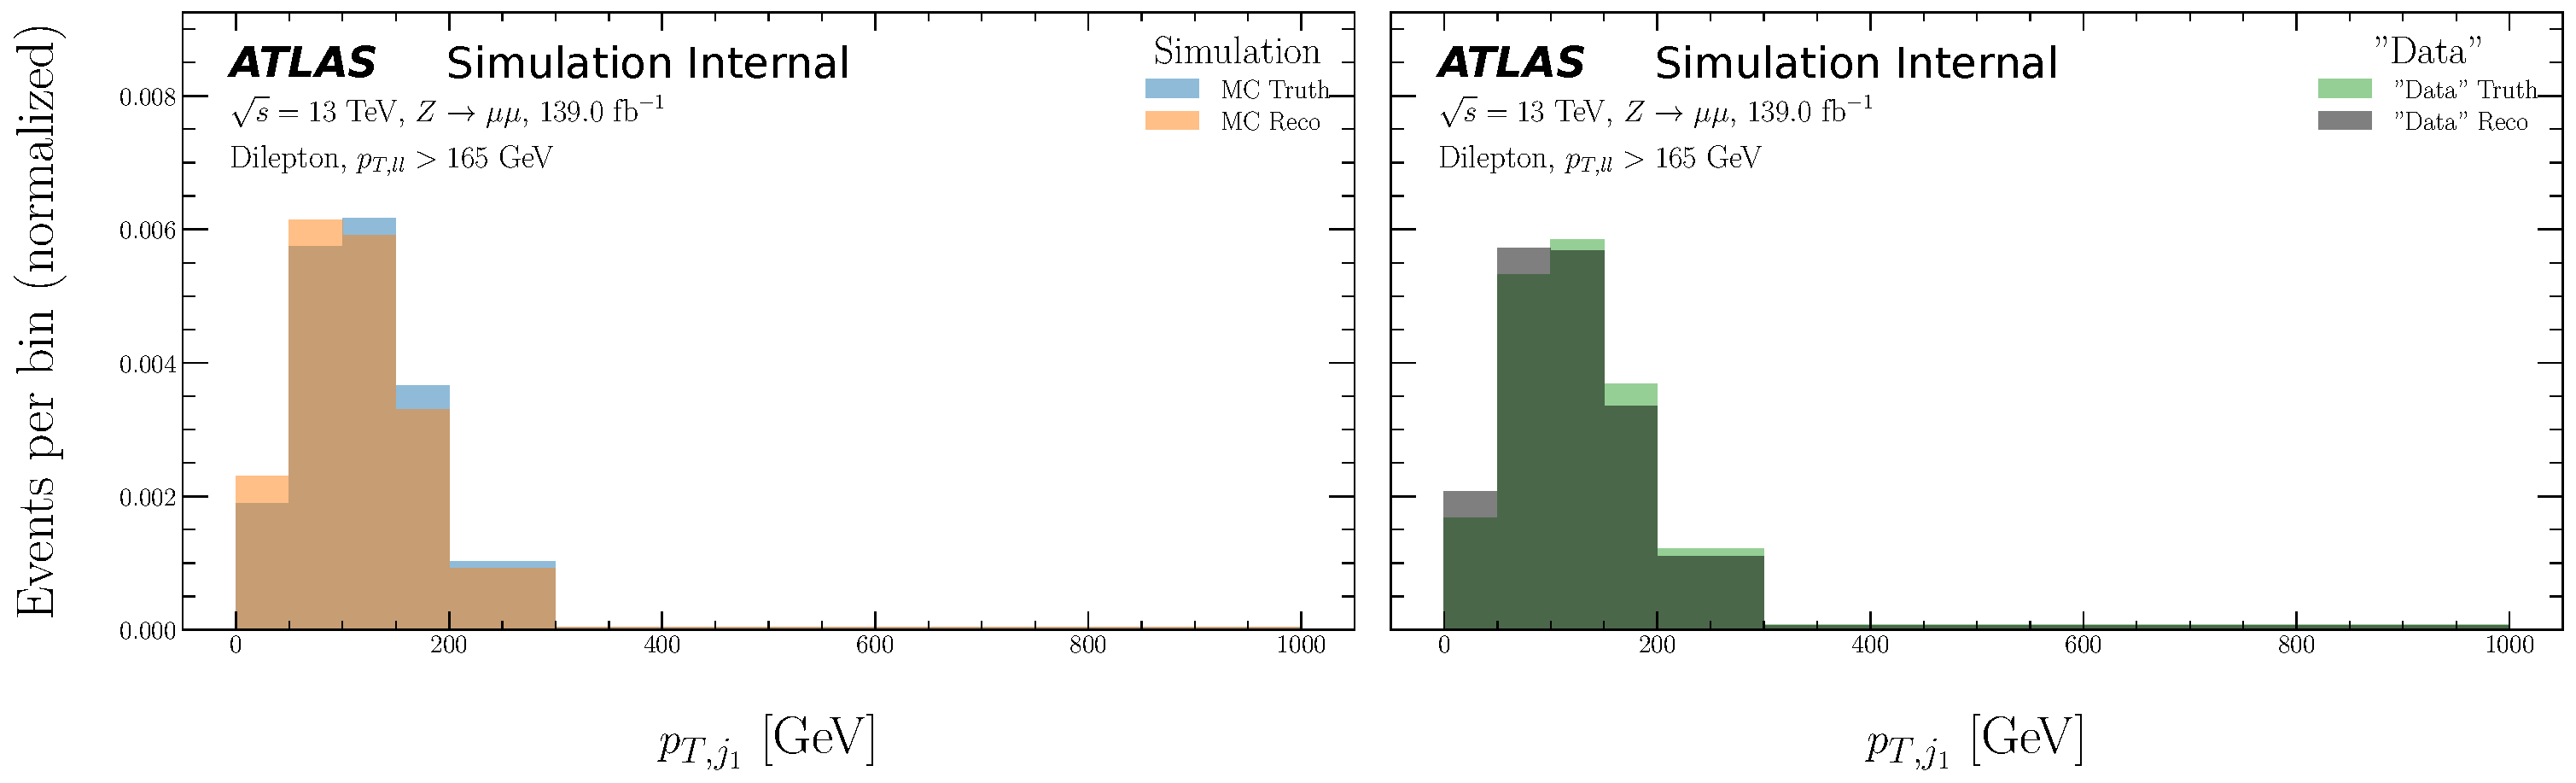
\includegraphics[width=0.85\textwidth]{figures/ATLASOmniFold-StressTest/ATLASOmniFold-StressTestA/MultiFold/pT_trackj1/ATLASOmniFold-StressTestA-MultiFold-pT_trackj1-Distributions}}\\
\subfloat[After 1 iteration]{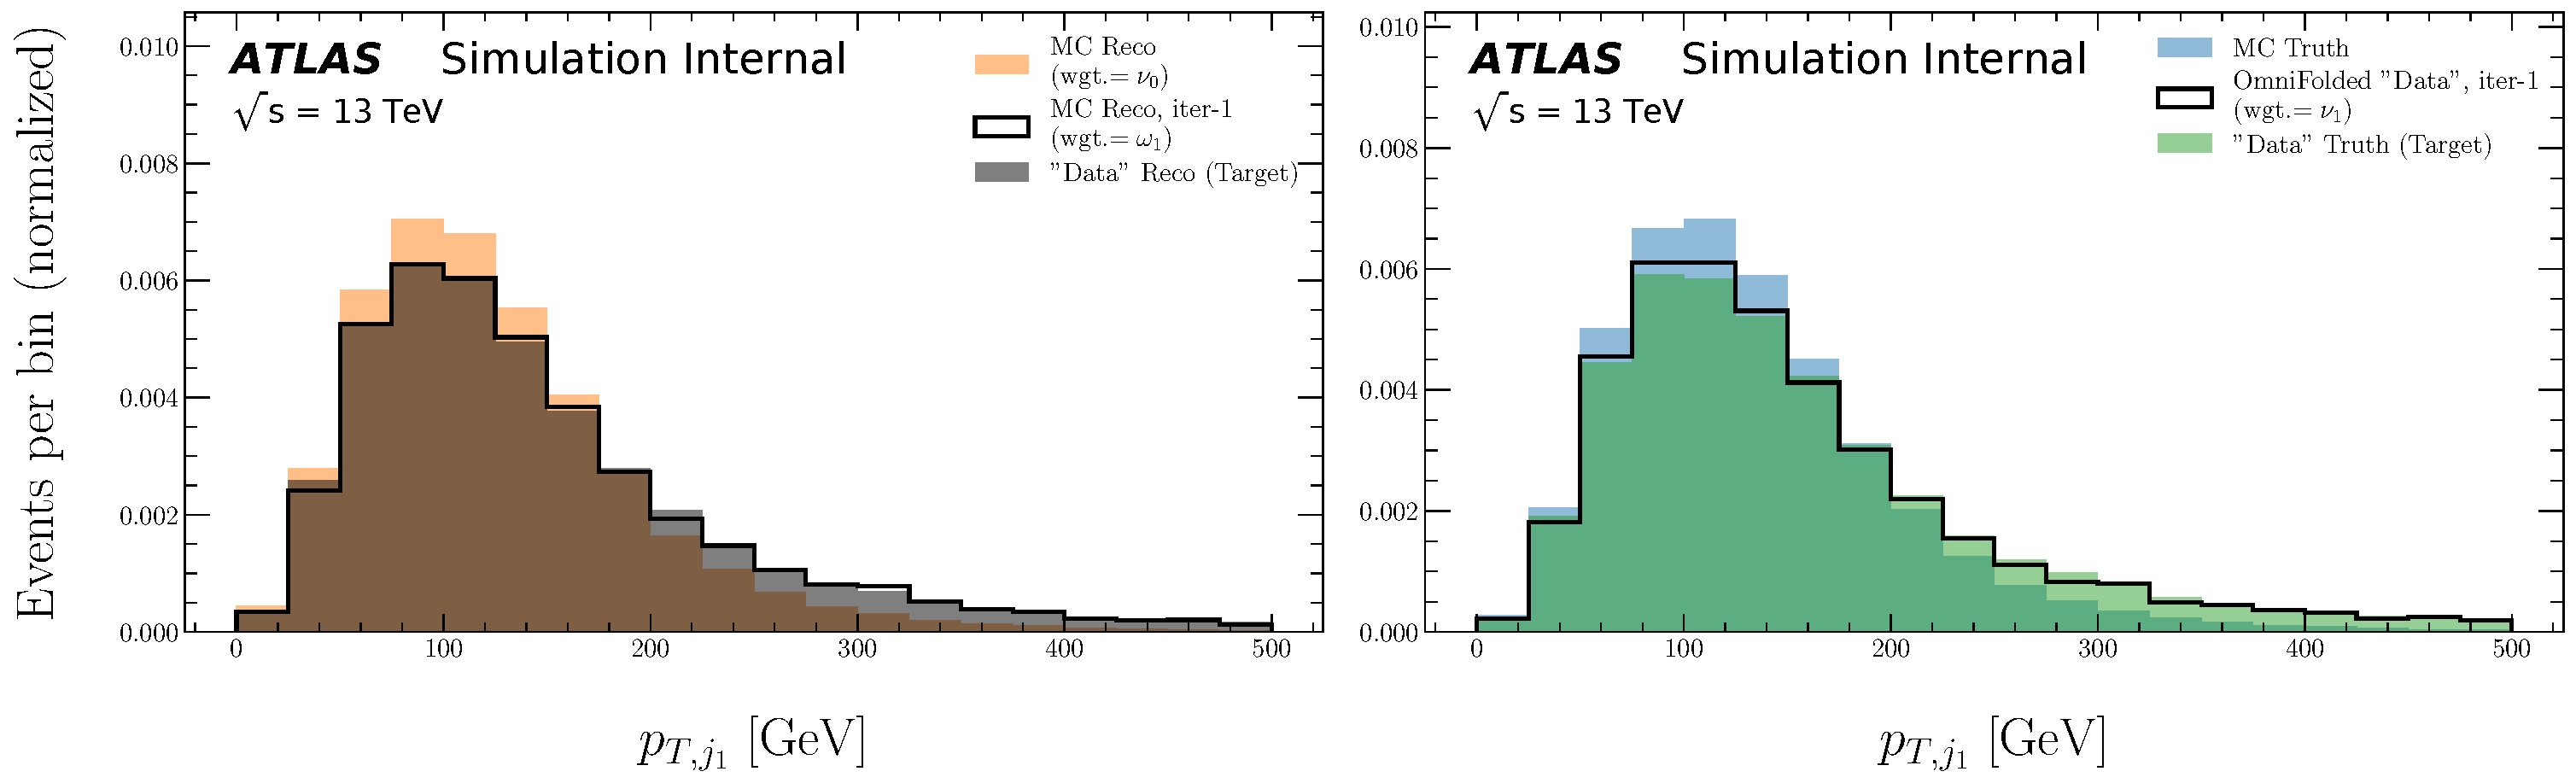
\includegraphics[width=0.85\textwidth]{figures/ATLASOmniFold-StressTest/ATLASOmniFold-StressTestA/MultiFold/pT_trackj1/ATLASOmniFold-StressTestA-MultiFold-pT_trackj1-Iteration01}}\\
\subfloat[After 2 iterations]{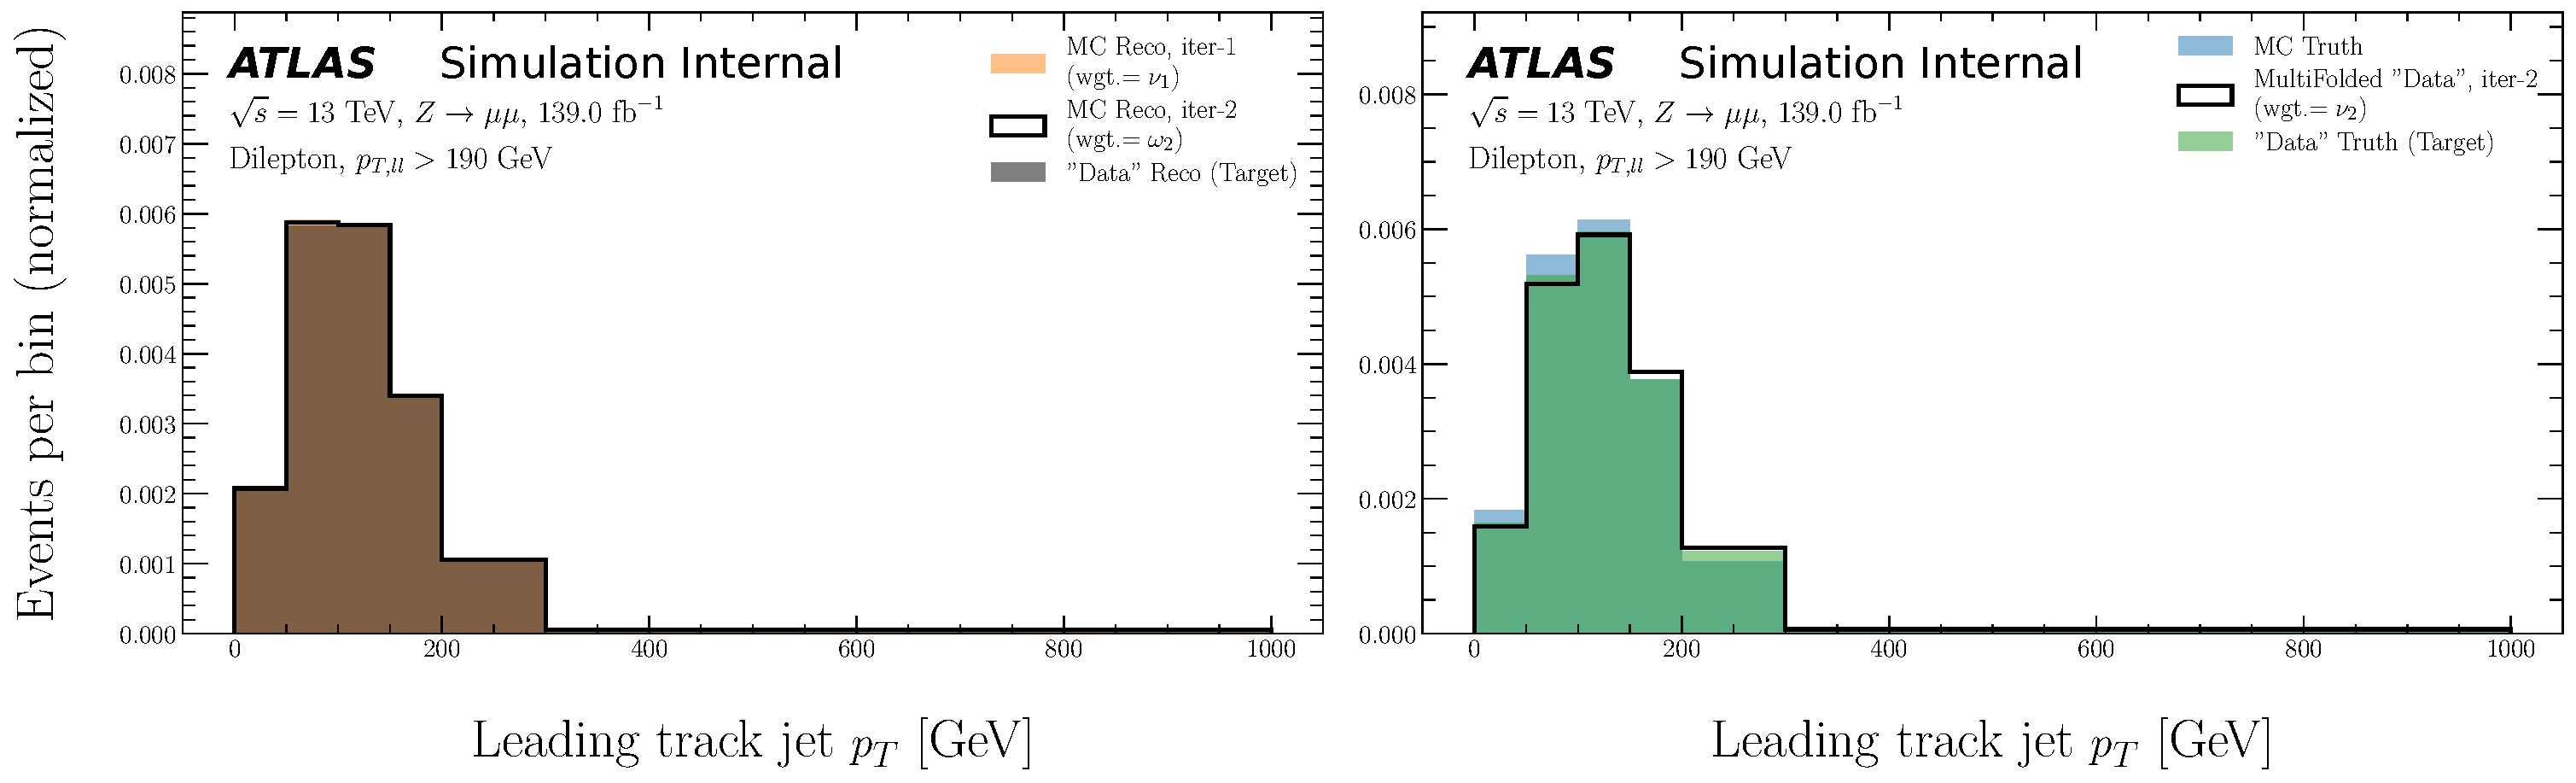
\includegraphics[width=0.85\textwidth]{figures/ATLASOmniFold-StressTest/ATLASOmniFold-StressTestA/MultiFold/pT_trackj1/ATLASOmniFold-StressTestA-MultiFold-pT_trackj1-Iteration02}}
\phantomcaption 
\end{figure}

\begin{figure}[h!]
\centering
\ContinuedFloat
\subfloat[After 3 iterations]{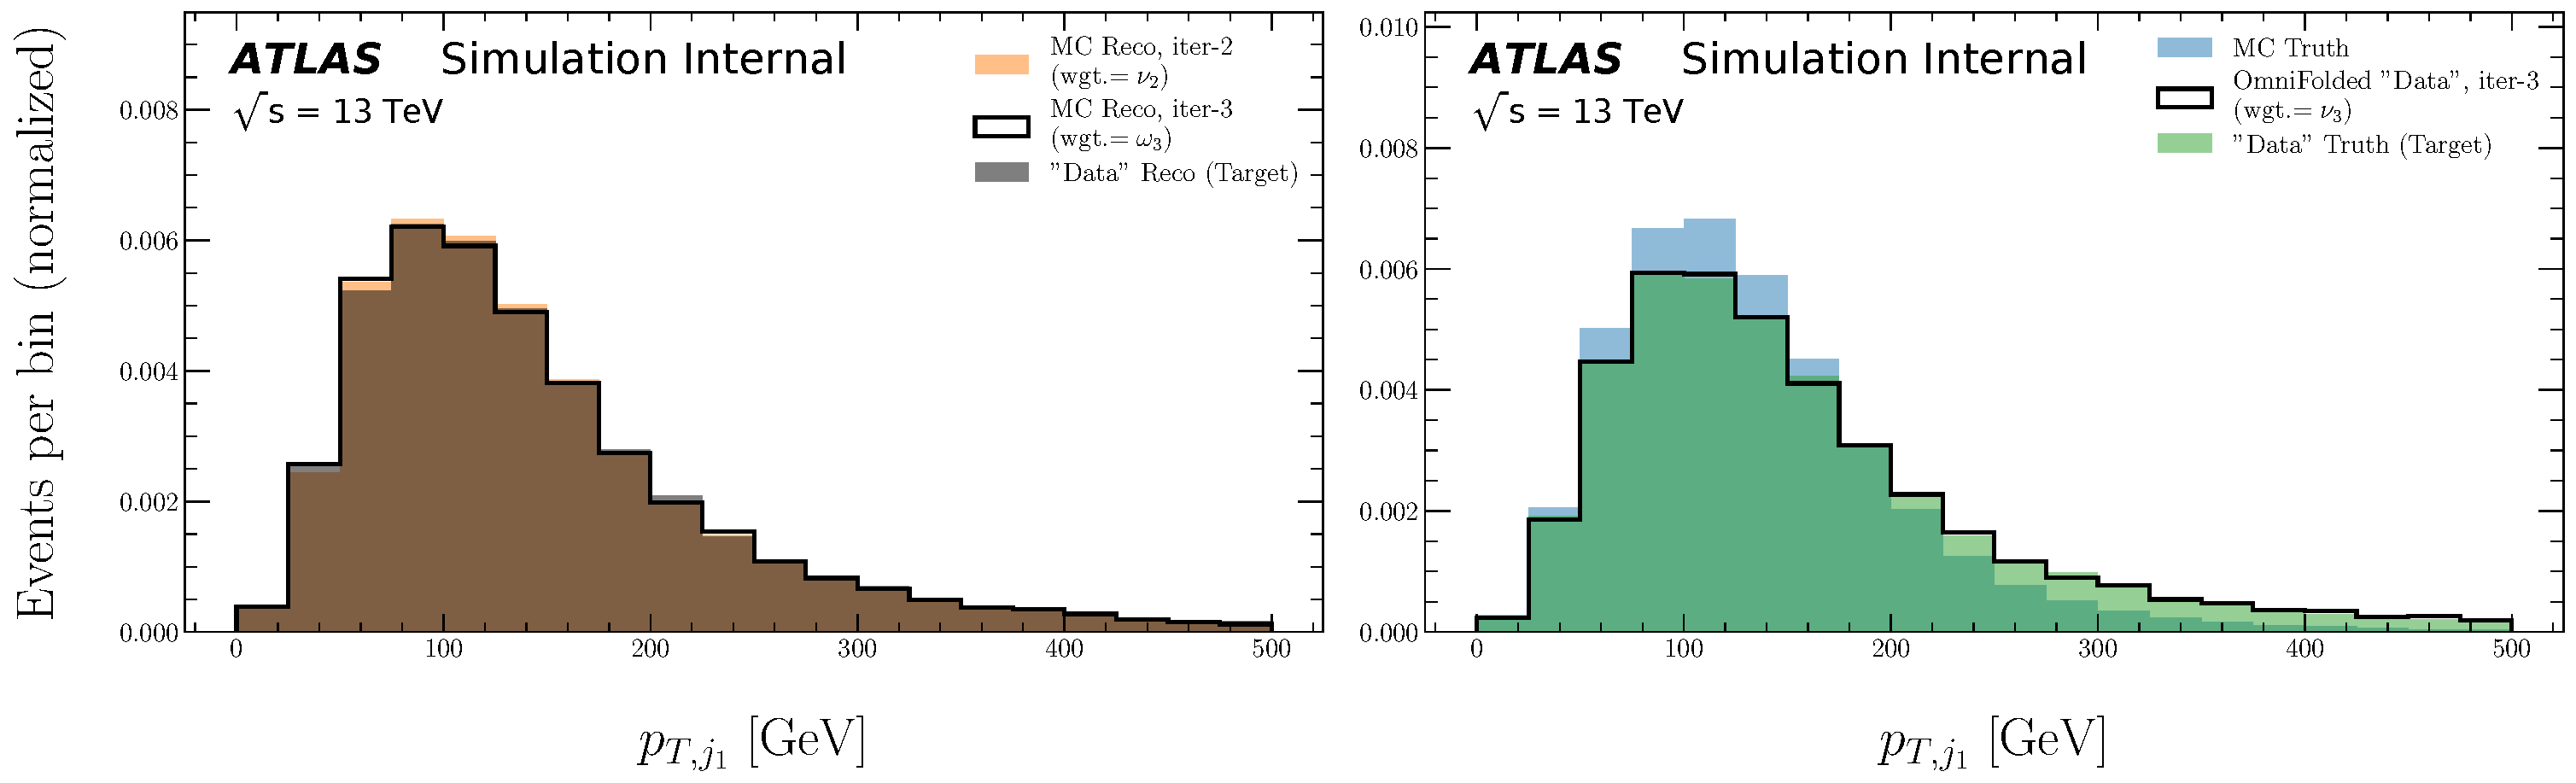
\includegraphics[width=0.85\textwidth]{figures/ATLASOmniFold-StressTest/ATLASOmniFold-StressTestA/MultiFold/pT_trackj1/ATLASOmniFold-StressTestA-MultiFold-pT_trackj1-Iteration03}}\\
\subfloat[After 4 iterations]{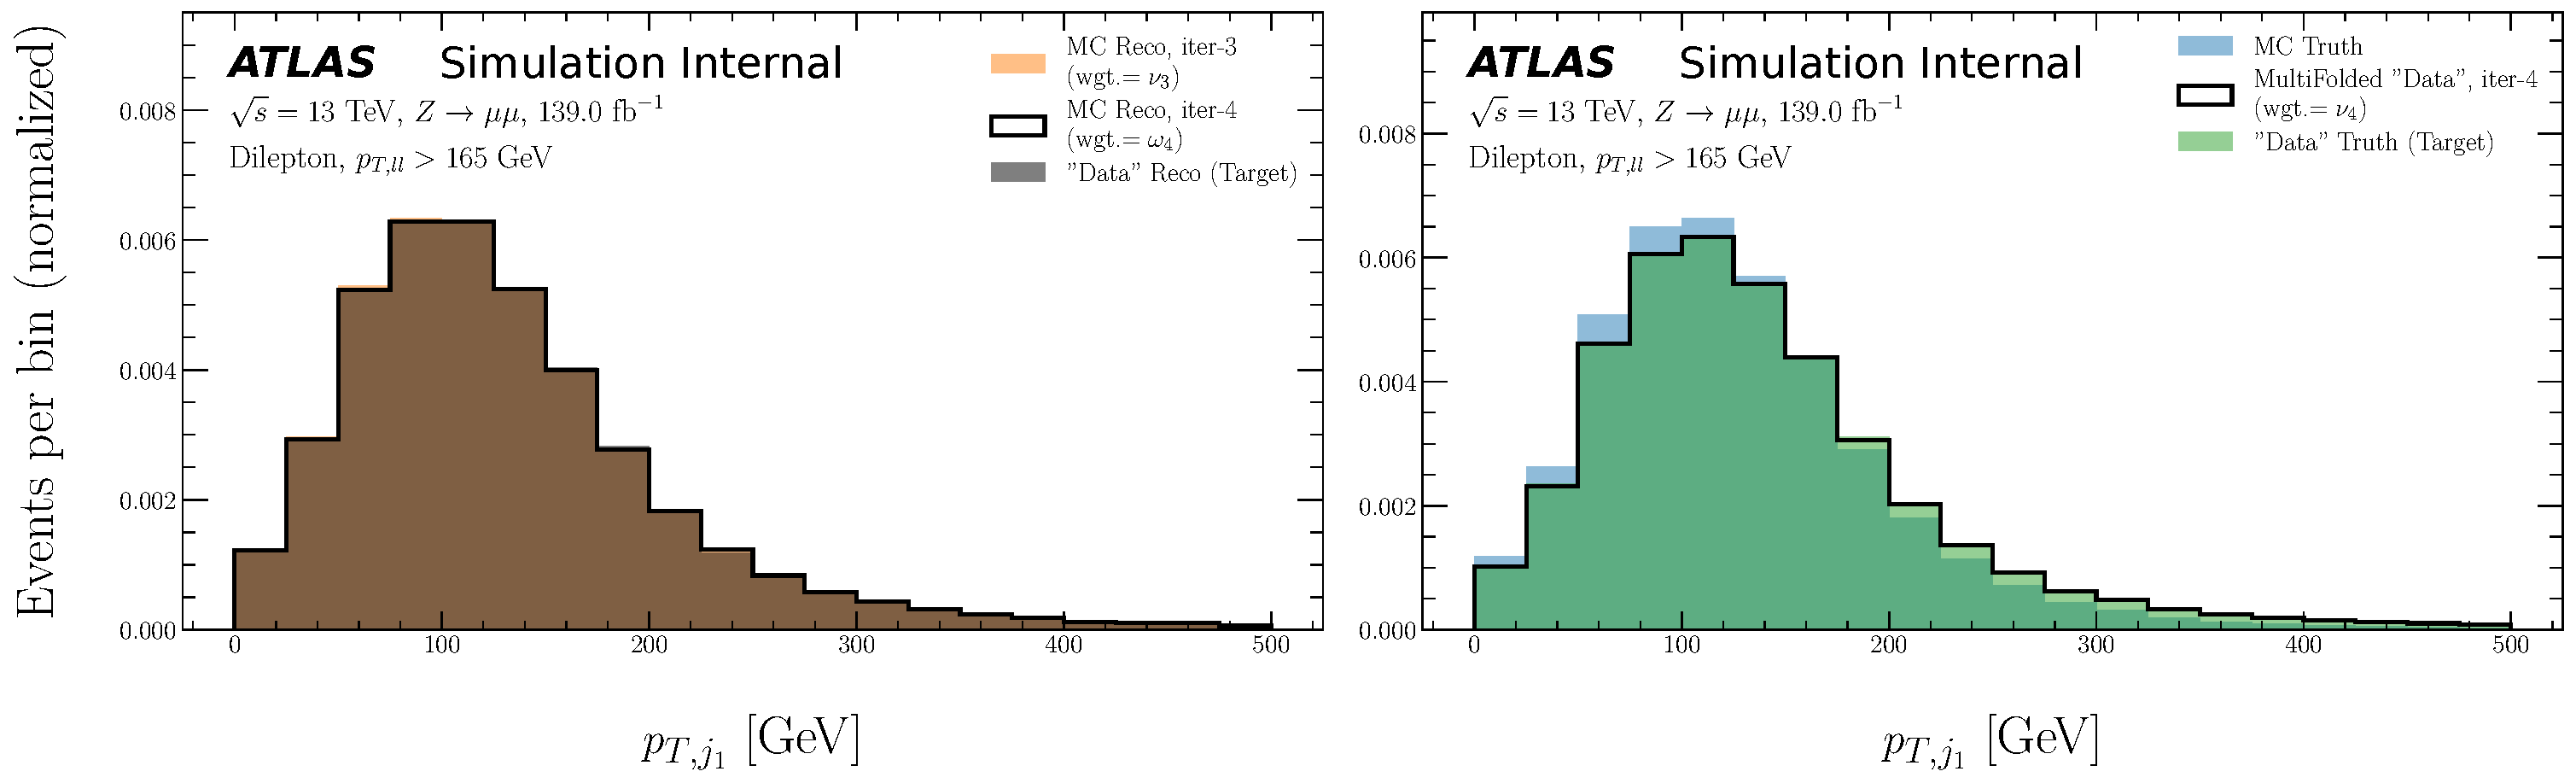
\includegraphics[width=0.85\textwidth]{figures/ATLASOmniFold-StressTest/ATLASOmniFold-StressTestA/MultiFold/pT_trackj1/ATLASOmniFold-StressTestA-MultiFold-pT_trackj1-Iteration04}}\\
\subfloat[After 5 iterations]{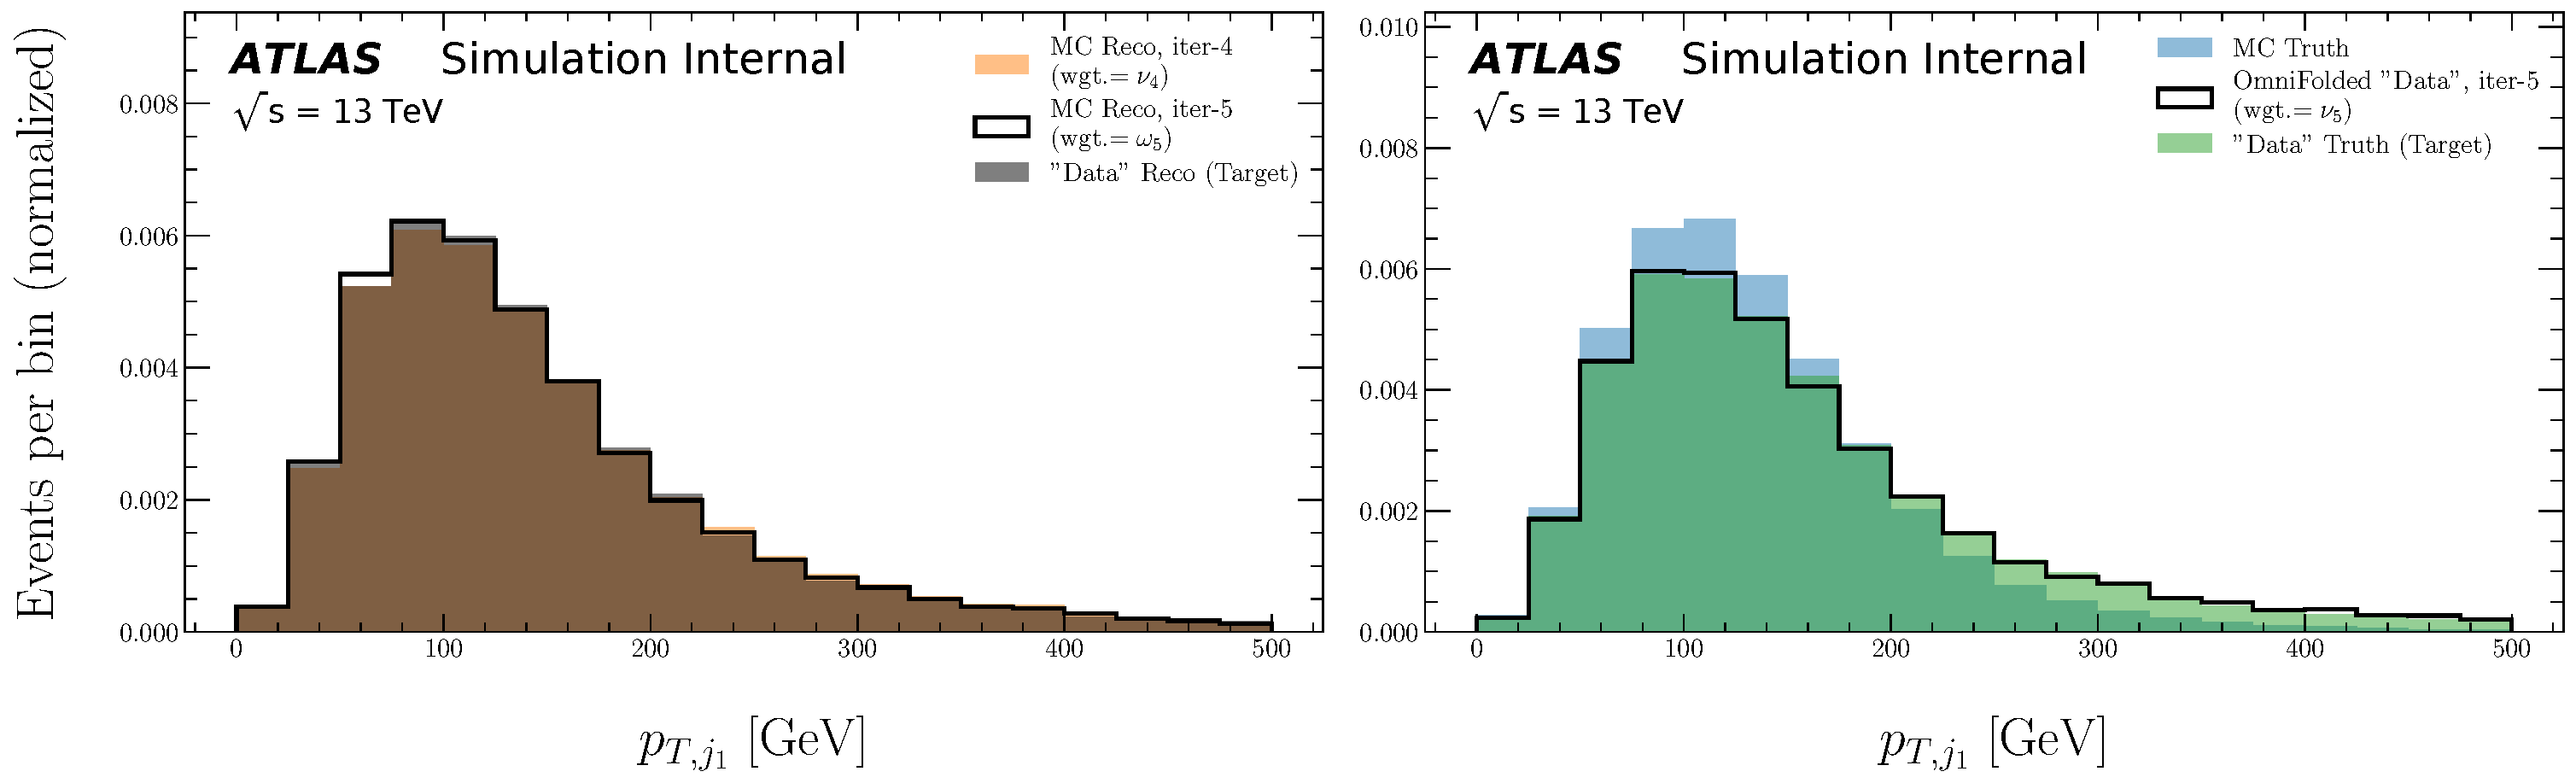
\includegraphics[width=0.85\textwidth]{figures/ATLASOmniFold-StressTest/ATLASOmniFold-StressTestA/MultiFold/pT_trackj1/ATLASOmniFold-StressTestA-MultiFold-pT_trackj1-Iteration05}}\\
\subfloat[After 6 iterations]{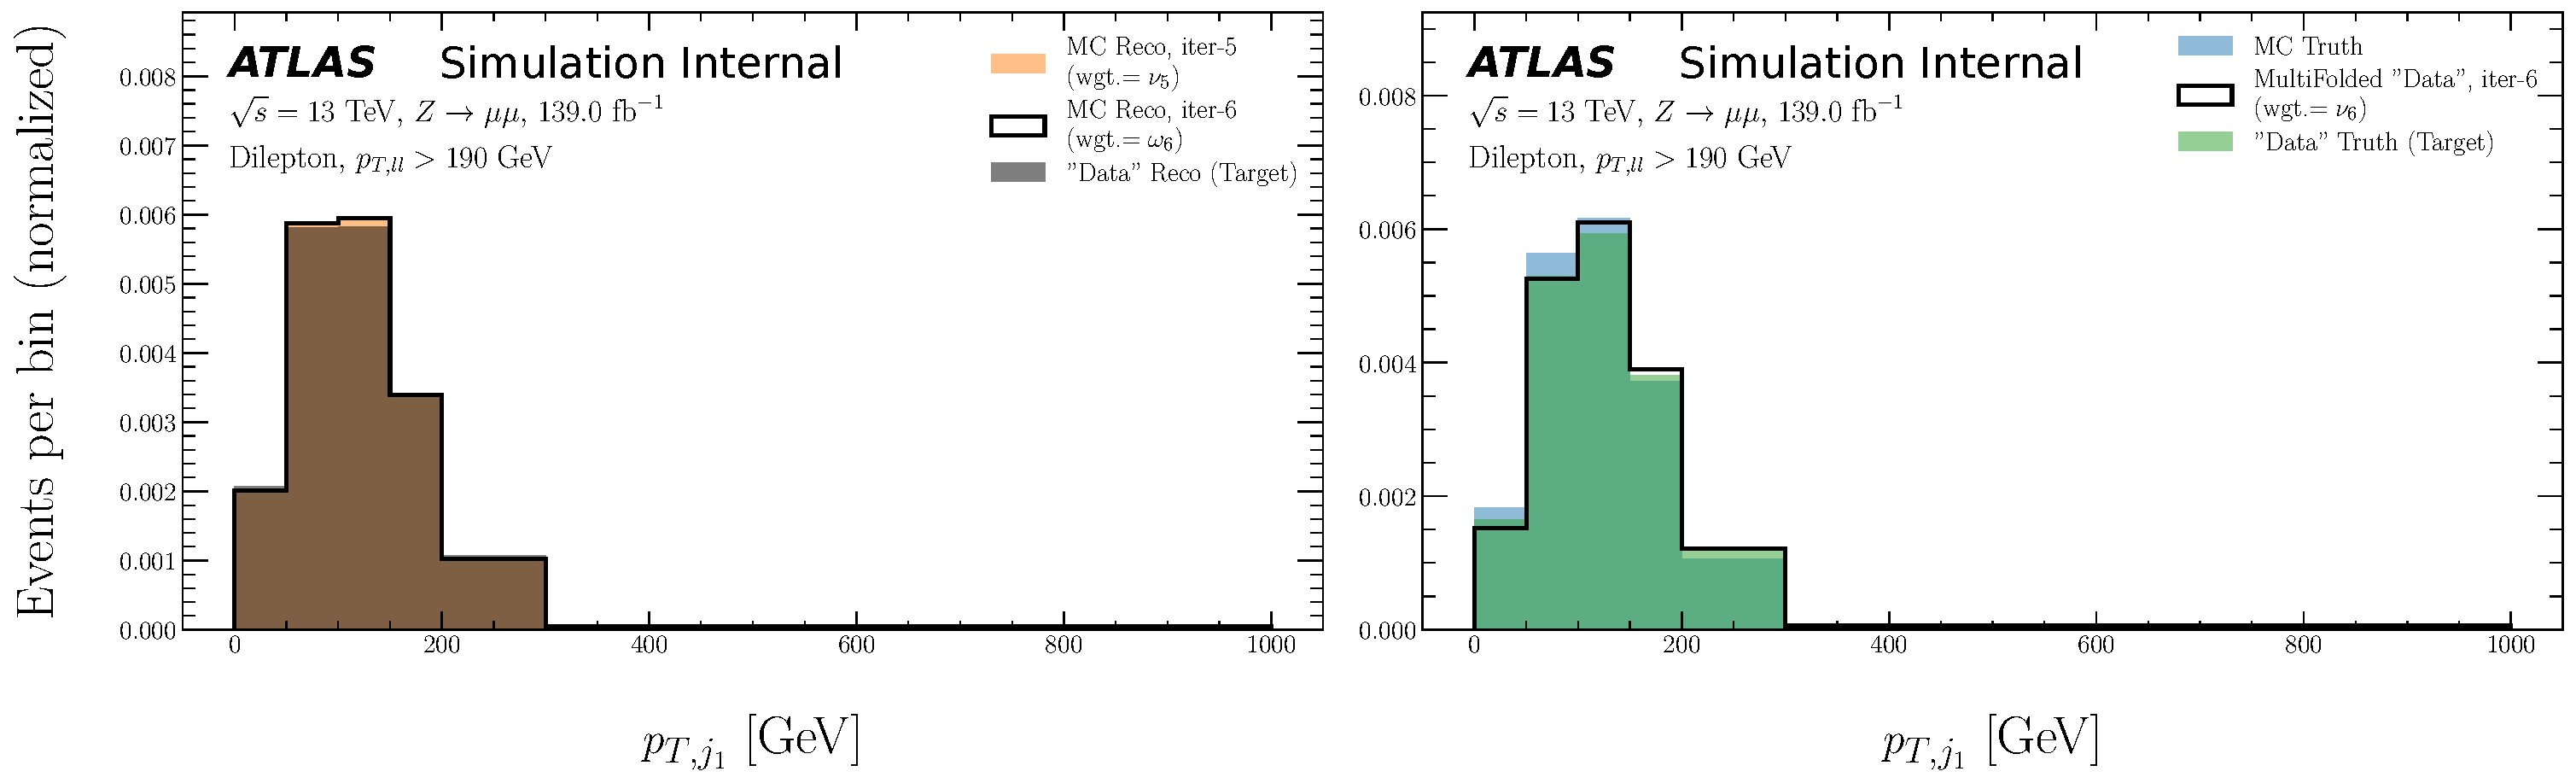
\includegraphics[width=0.85\textwidth]{figures/ATLASOmniFold-StressTest/ATLASOmniFold-StressTestA/MultiFold/pT_trackj1/ATLASOmniFold-StressTestA-MultiFold-pT_trackj1-Iteration06}}
\caption{A stress test for MultiFold using deterministic weights applied to the leading track jet $p_T$.}
\label{fig:stressa_pT_trackj1Multi}
\end{figure}

\begin{figure}[h!]
\centering
\subfloat[Input histograms]{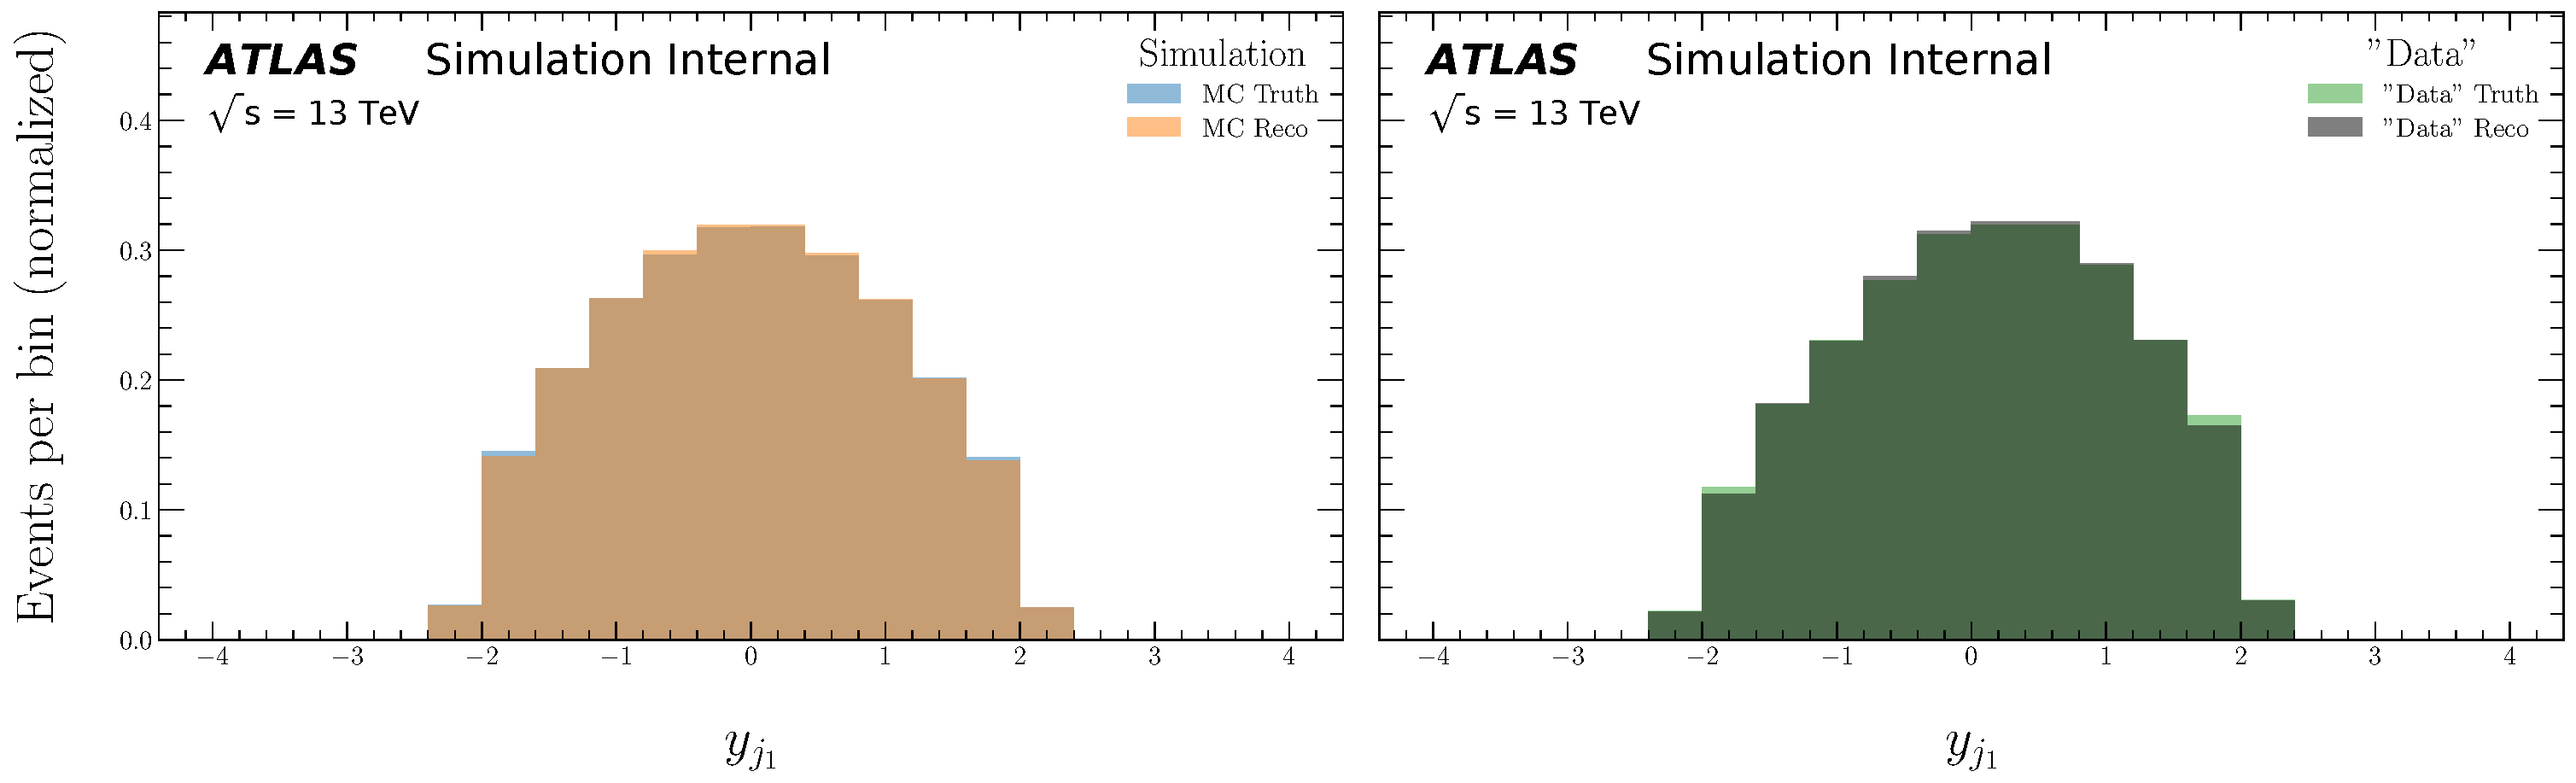
\includegraphics[width=0.85\textwidth]{figures/ATLASOmniFold-StressTest/ATLASOmniFold-StressTestA/MultiFold/y_trackj1/ATLASOmniFold-StressTestA-MultiFold-y_trackj1-Distributions}}\\
\subfloat[After 1 iteration]{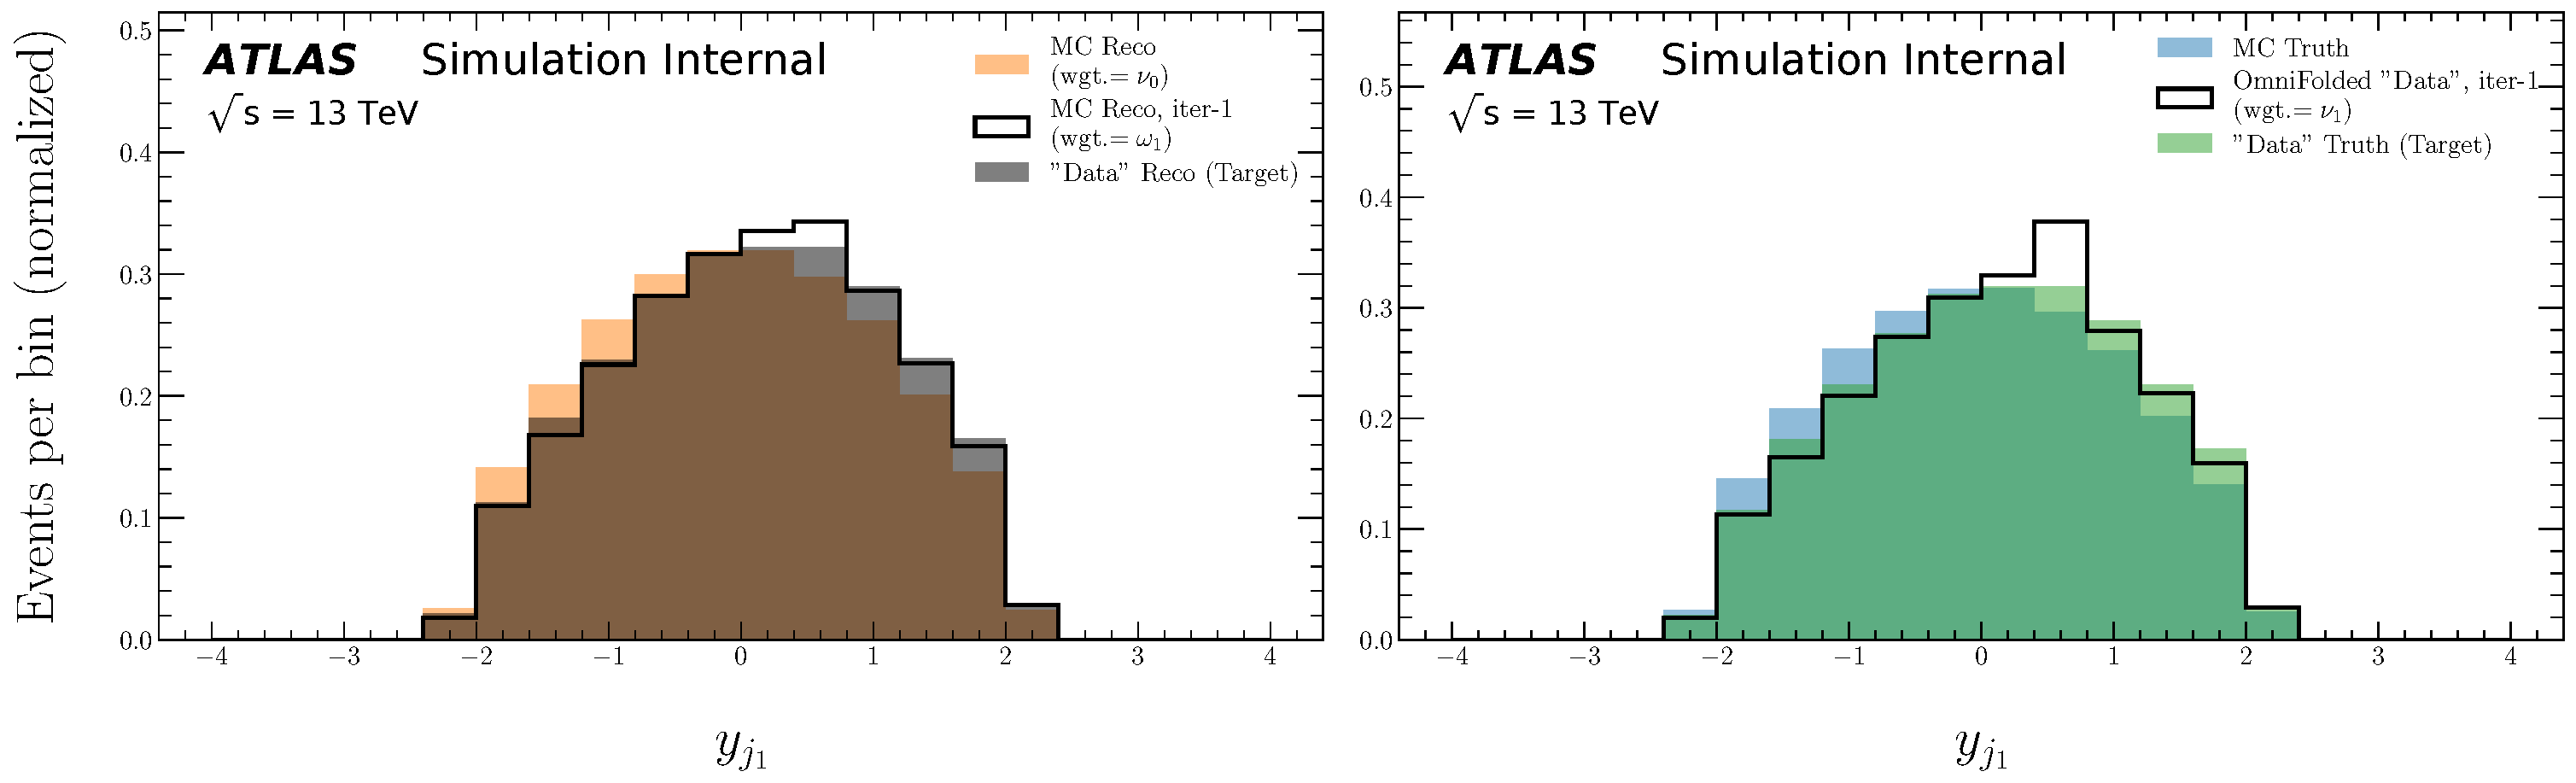
\includegraphics[width=0.85\textwidth]{figures/ATLASOmniFold-StressTest/ATLASOmniFold-StressTestA/MultiFold/y_trackj1/ATLASOmniFold-StressTestA-MultiFold-y_trackj1-Iteration01}}\\
\subfloat[After 2 iterations]{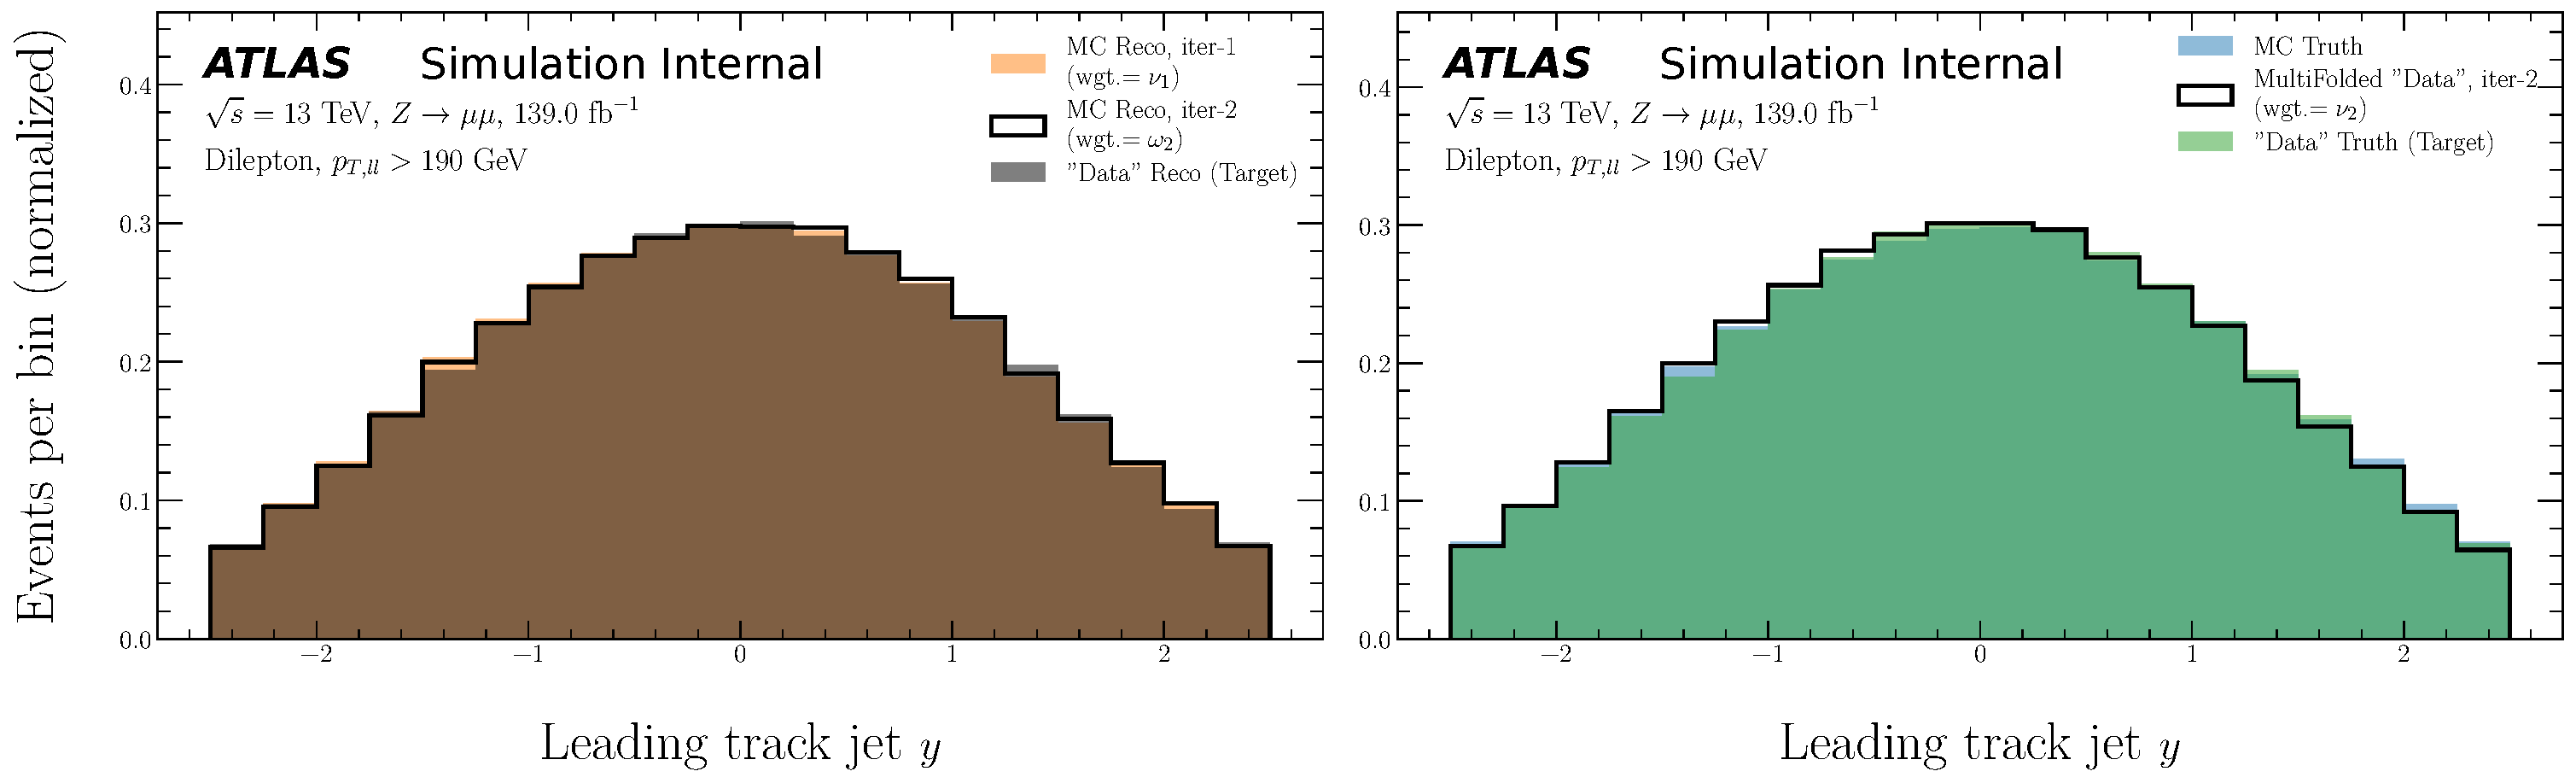
\includegraphics[width=0.85\textwidth]{figures/ATLASOmniFold-StressTest/ATLASOmniFold-StressTestA/MultiFold/y_trackj1/ATLASOmniFold-StressTestA-MultiFold-y_trackj1-Iteration02}}
\phantomcaption 
\end{figure}

\begin{figure}[h!]
\centering
\ContinuedFloat
\subfloat[After 3 iterations]{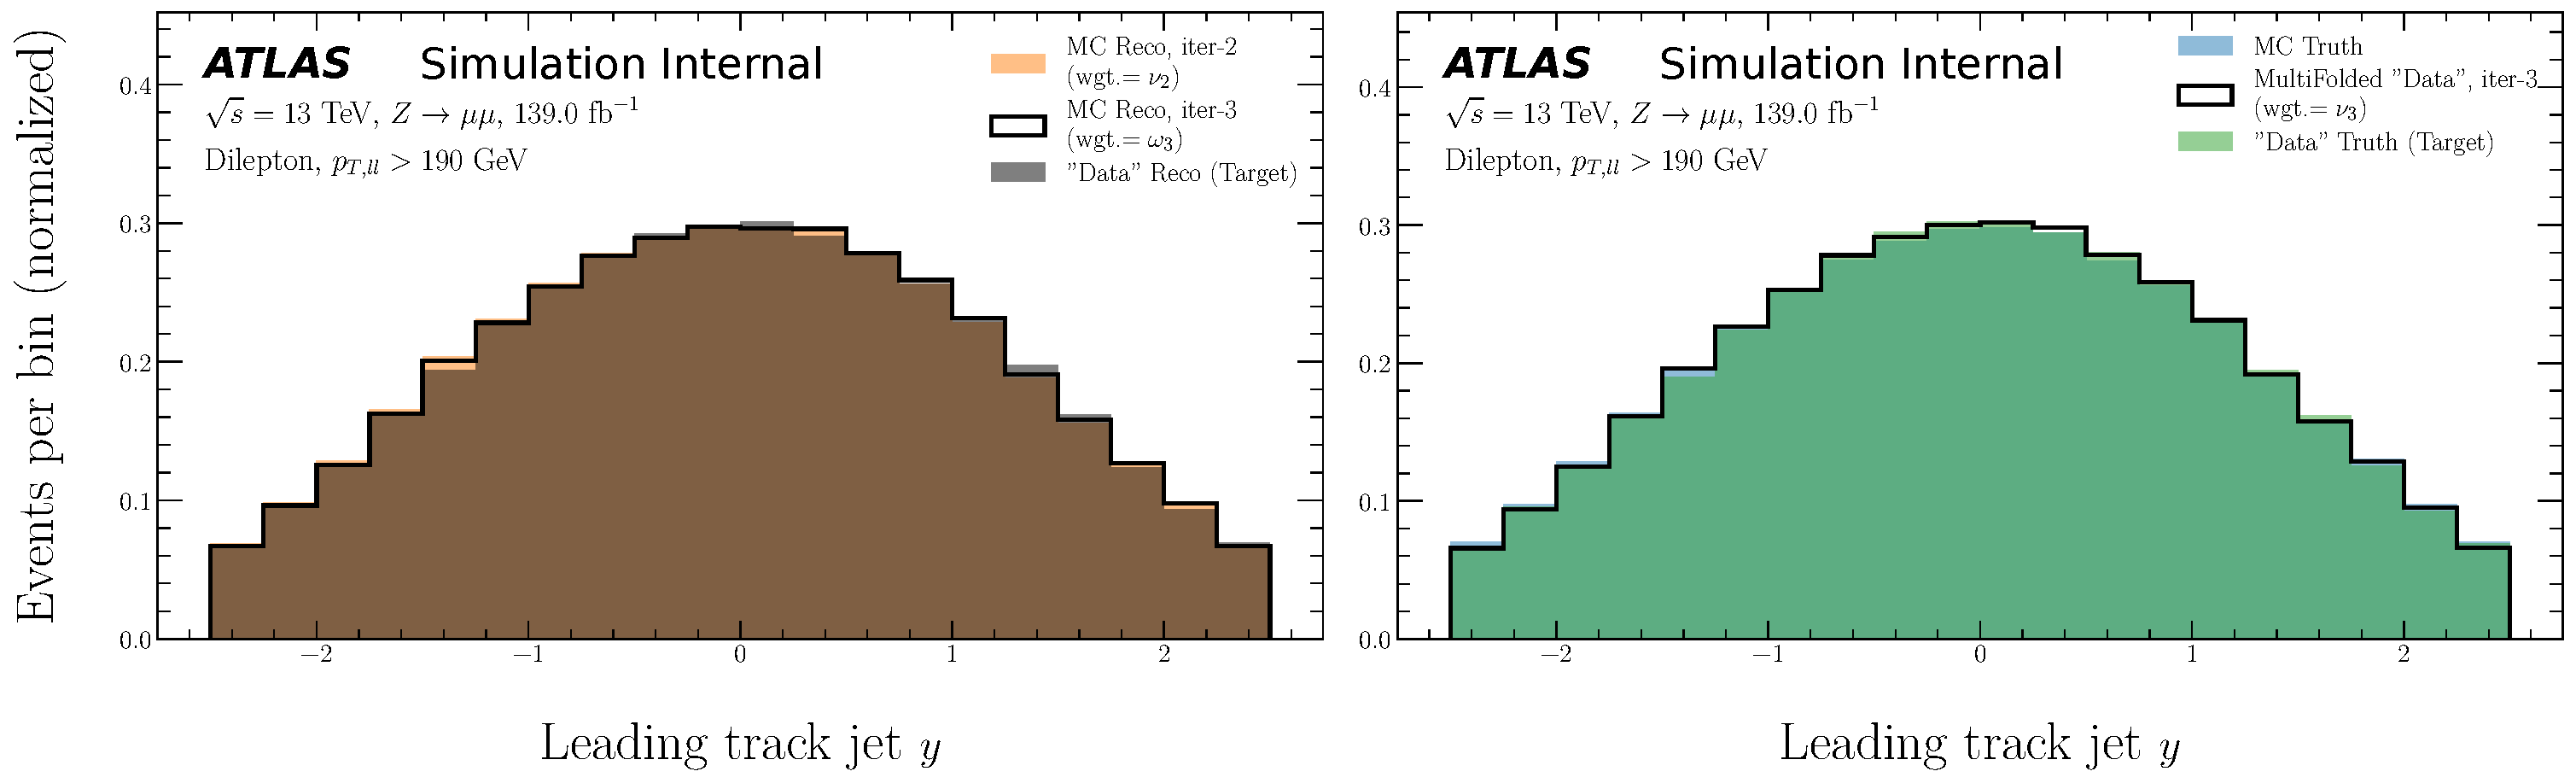
\includegraphics[width=0.85\textwidth]{figures/ATLASOmniFold-StressTest/ATLASOmniFold-StressTestA/MultiFold/y_trackj1/ATLASOmniFold-StressTestA-MultiFold-y_trackj1-Iteration03}}\\
\subfloat[After 4 iterations]{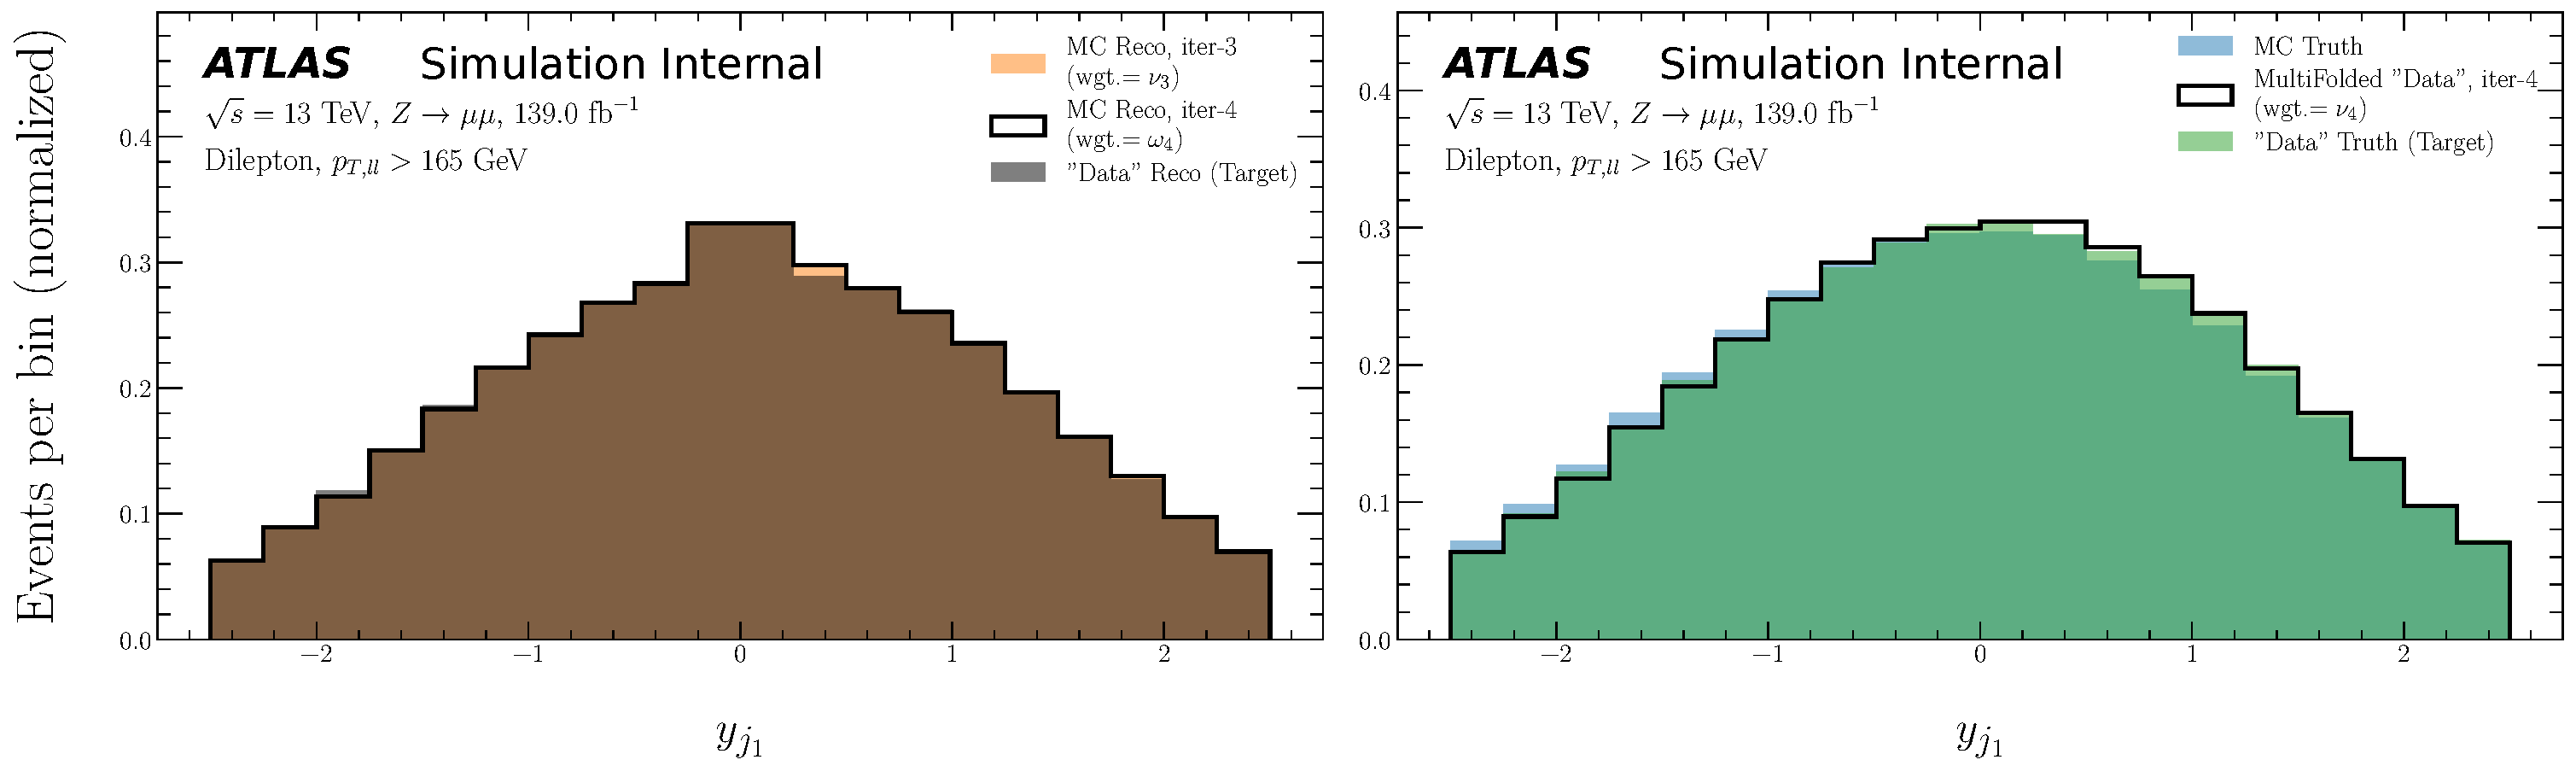
\includegraphics[width=0.85\textwidth]{figures/ATLASOmniFold-StressTest/ATLASOmniFold-StressTestA/MultiFold/y_trackj1/ATLASOmniFold-StressTestA-MultiFold-y_trackj1-Iteration04}}\\
\subfloat[After 5 iterations]{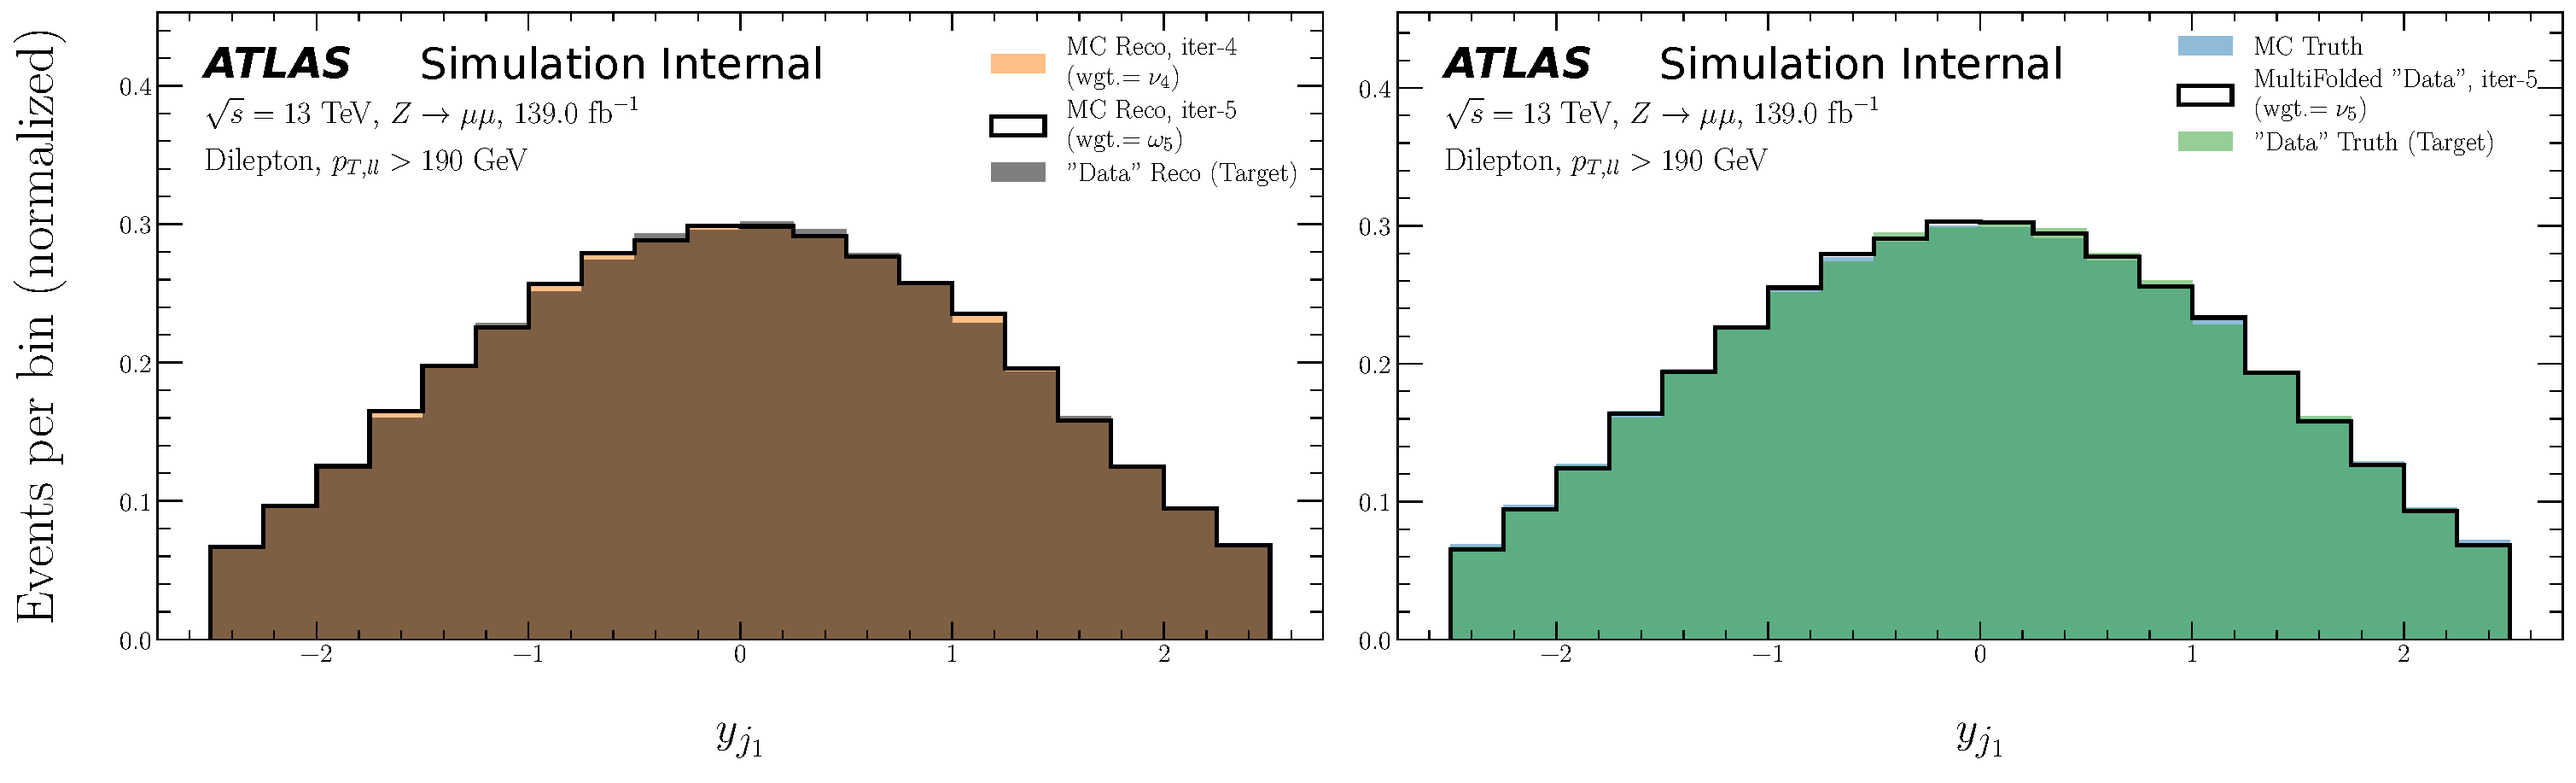
\includegraphics[width=0.85\textwidth]{figures/ATLASOmniFold-StressTest/ATLASOmniFold-StressTestA/MultiFold/y_trackj1/ATLASOmniFold-StressTestA-MultiFold-y_trackj1-Iteration05}}\\
\subfloat[After 6 iterations]{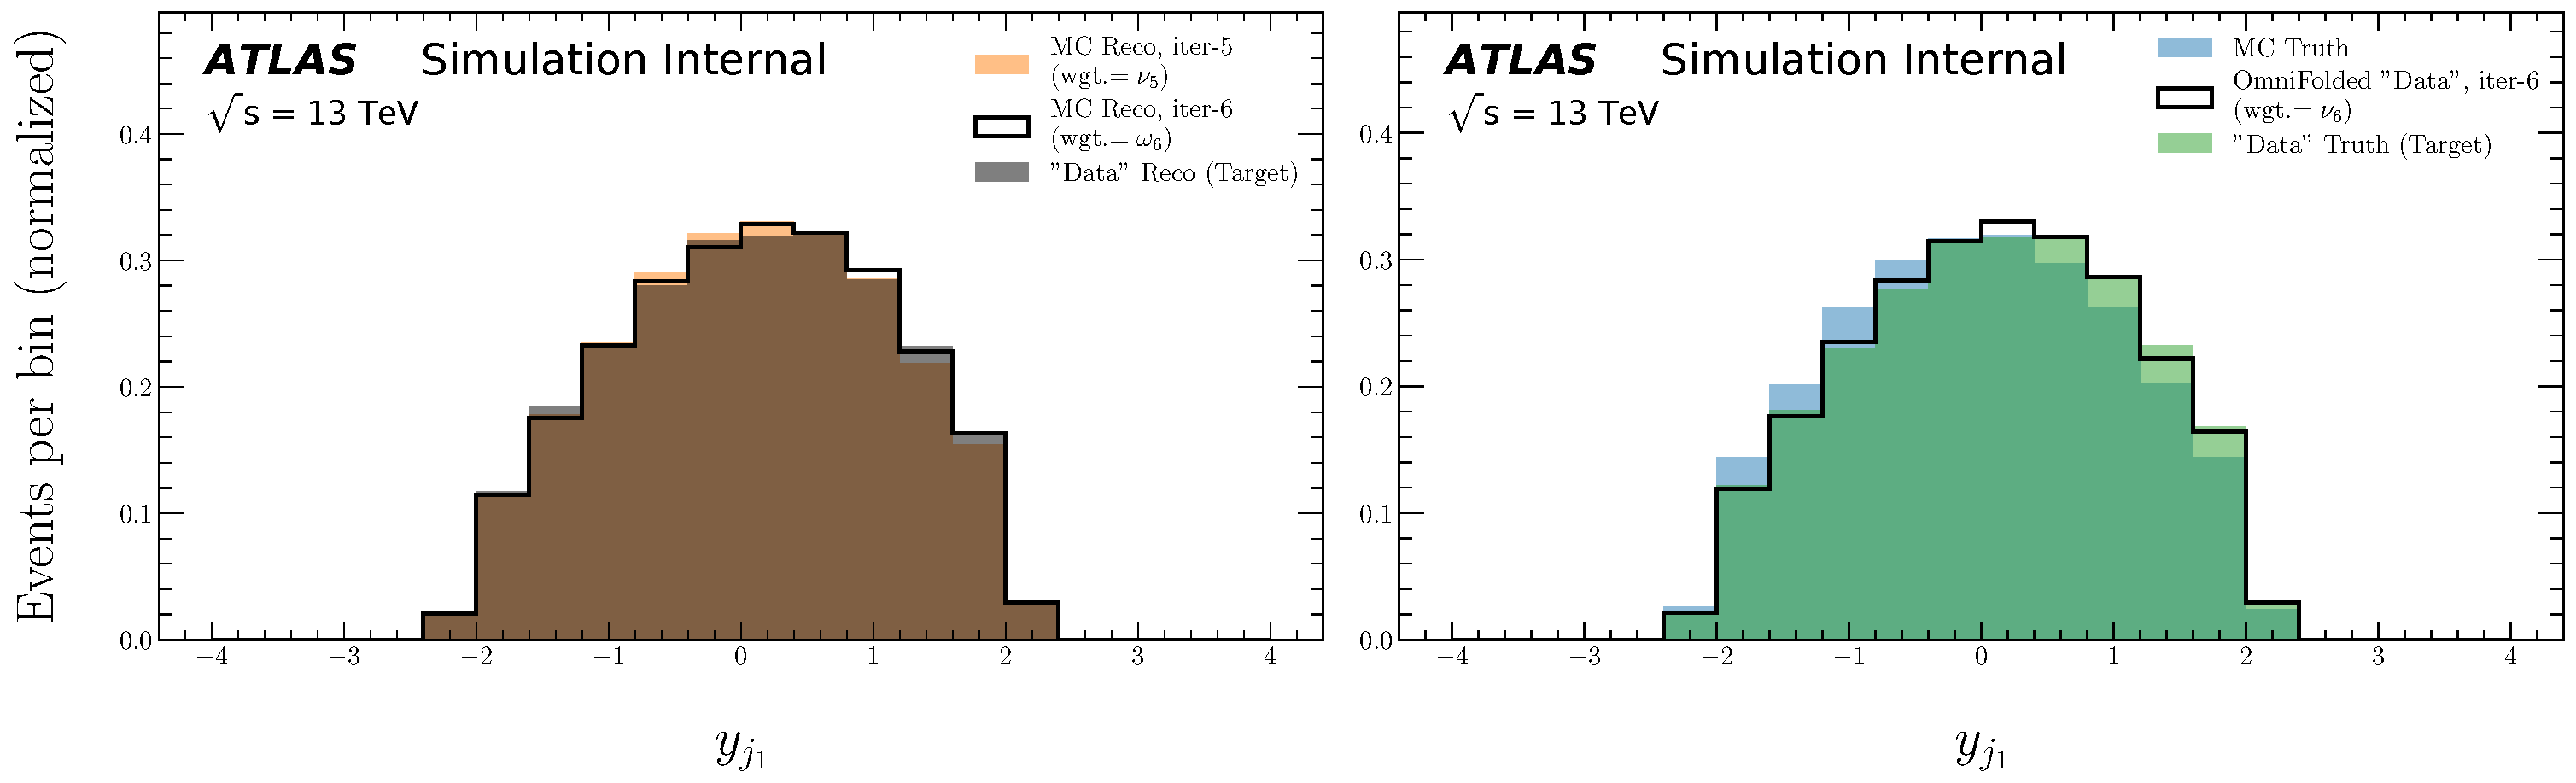
\includegraphics[width=0.85\textwidth]{figures/ATLASOmniFold-StressTest/ATLASOmniFold-StressTestA/MultiFold/y_trackj1/ATLASOmniFold-StressTestA-MultiFold-y_trackj1-Iteration06}}
\caption{A stress test for MultiFold using deterministic weights applied to the leading track jet rapidity.}
\label{fig:stressa_y_trackj1Multi}
\end{figure}

\begin{figure}[h!]
\centering
\subfloat[Input histograms]{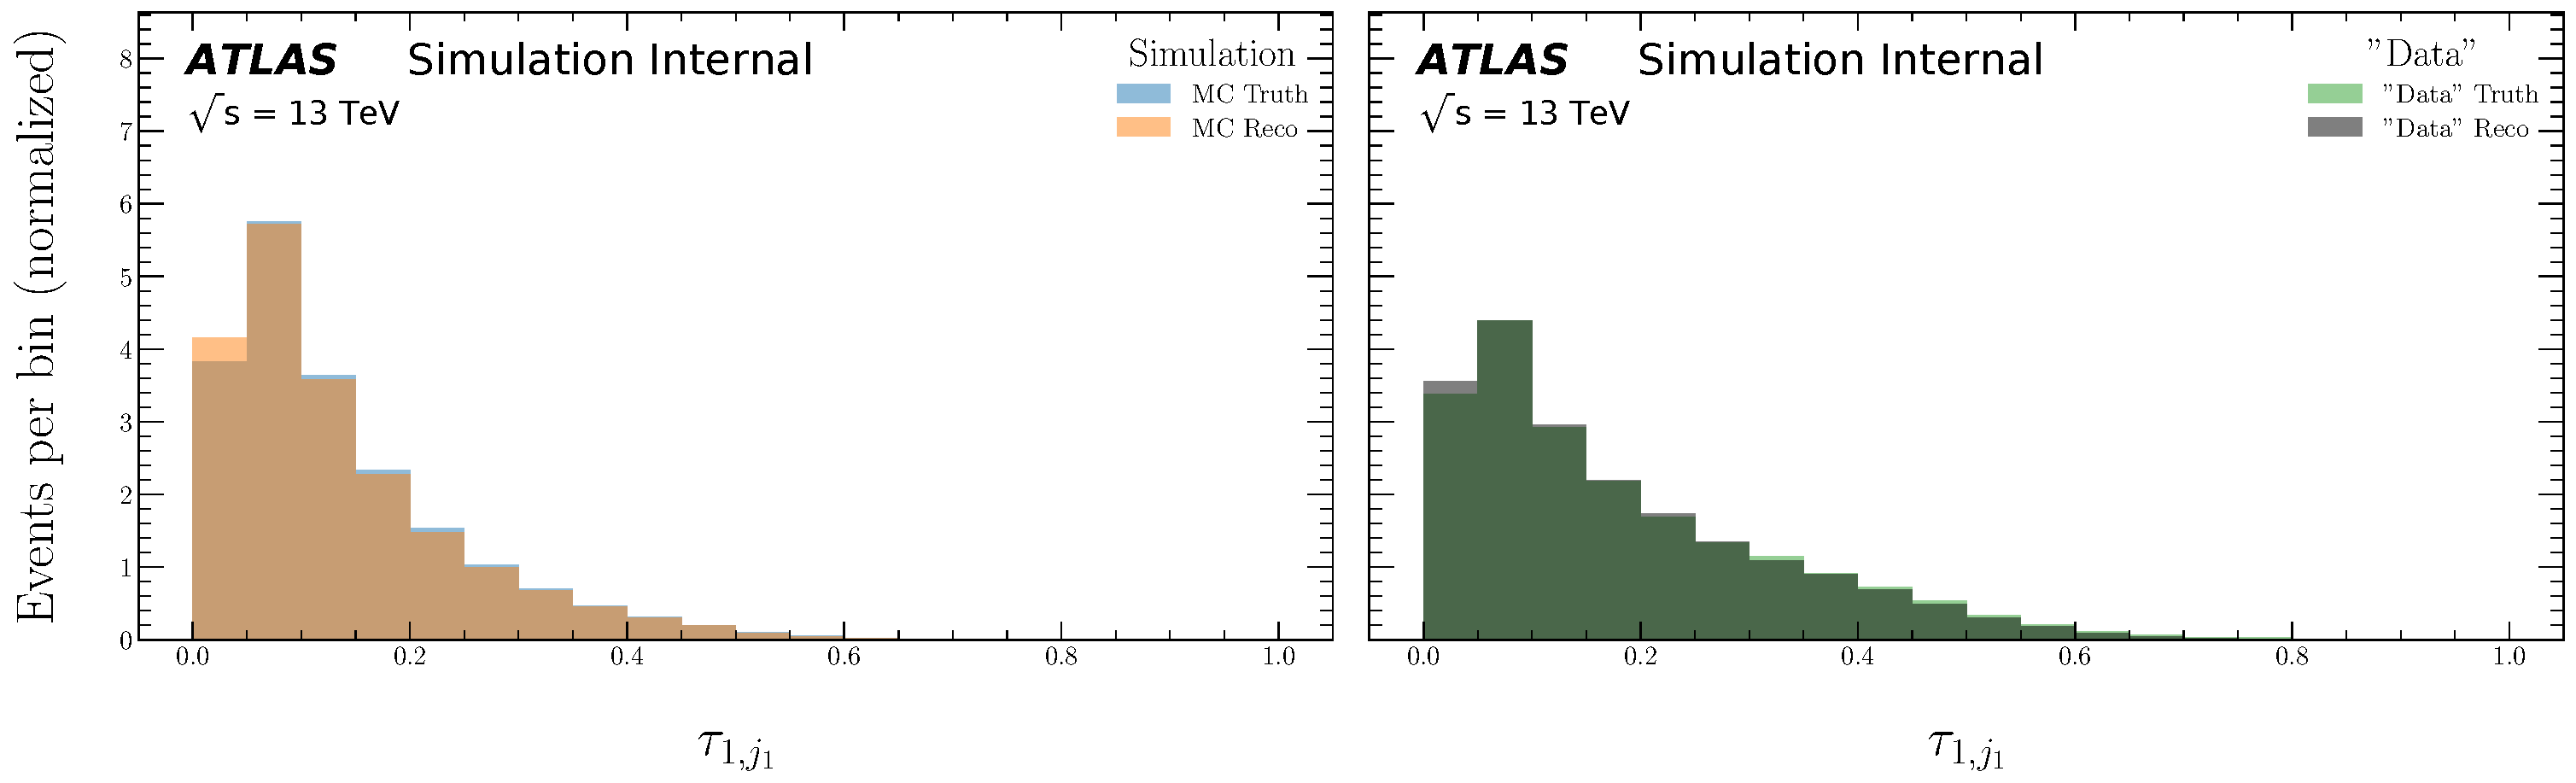
\includegraphics[width=0.85\textwidth]{figures/ATLASOmniFold-StressTest/ATLASOmniFold-StressTestA/MultiFold/tau1_trackj1/ATLASOmniFold-StressTestA-MultiFold-tau1_trackj1-Distributions}}\\
\subfloat[After 1 iteration]{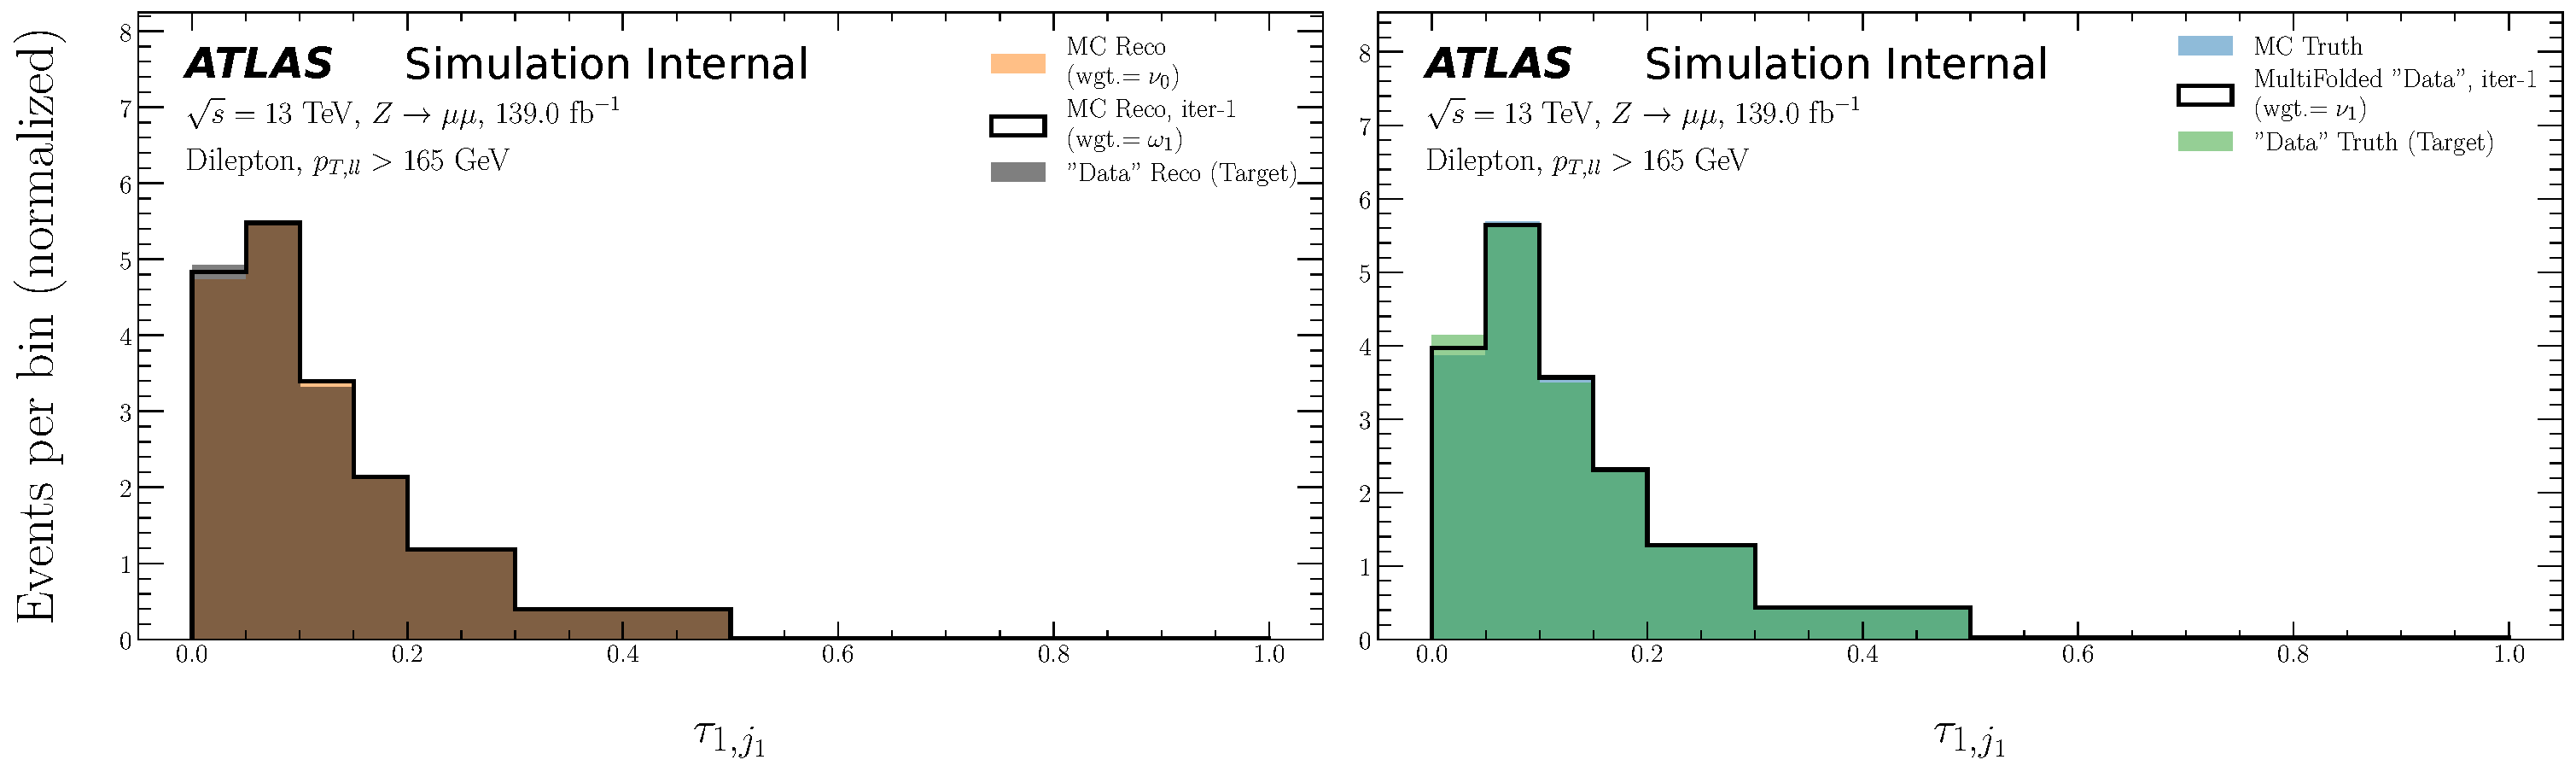
\includegraphics[width=0.85\textwidth]{figures/ATLASOmniFold-StressTest/ATLASOmniFold-StressTestA/MultiFold/tau1_trackj1/ATLASOmniFold-StressTestA-MultiFold-tau1_trackj1-Iteration01}}\\
\subfloat[After 2 iterations]{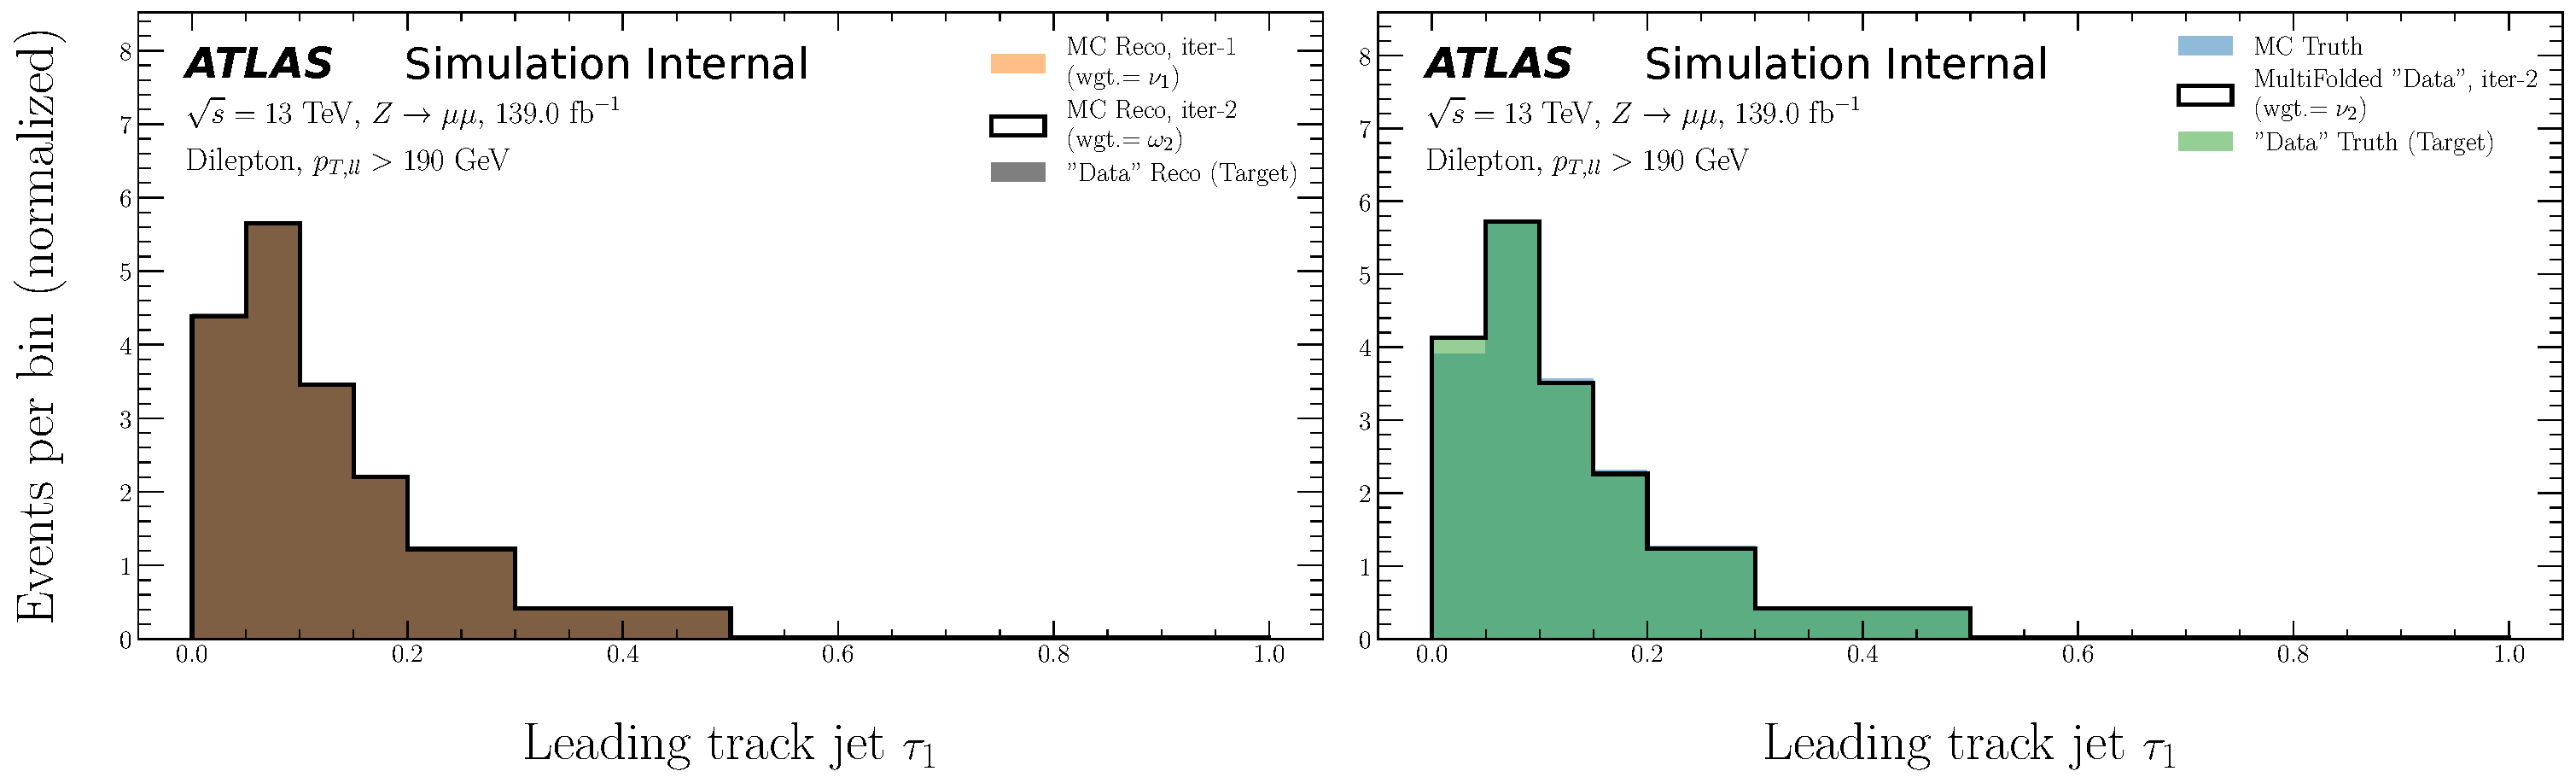
\includegraphics[width=0.85\textwidth]{figures/ATLASOmniFold-StressTest/ATLASOmniFold-StressTestA/MultiFold/tau1_trackj1/ATLASOmniFold-StressTestA-MultiFold-tau1_trackj1-Iteration02}}
\phantomcaption 
\end{figure}

\begin{figure}[h!]
\centering
\ContinuedFloat
\subfloat[After 3 iterations]{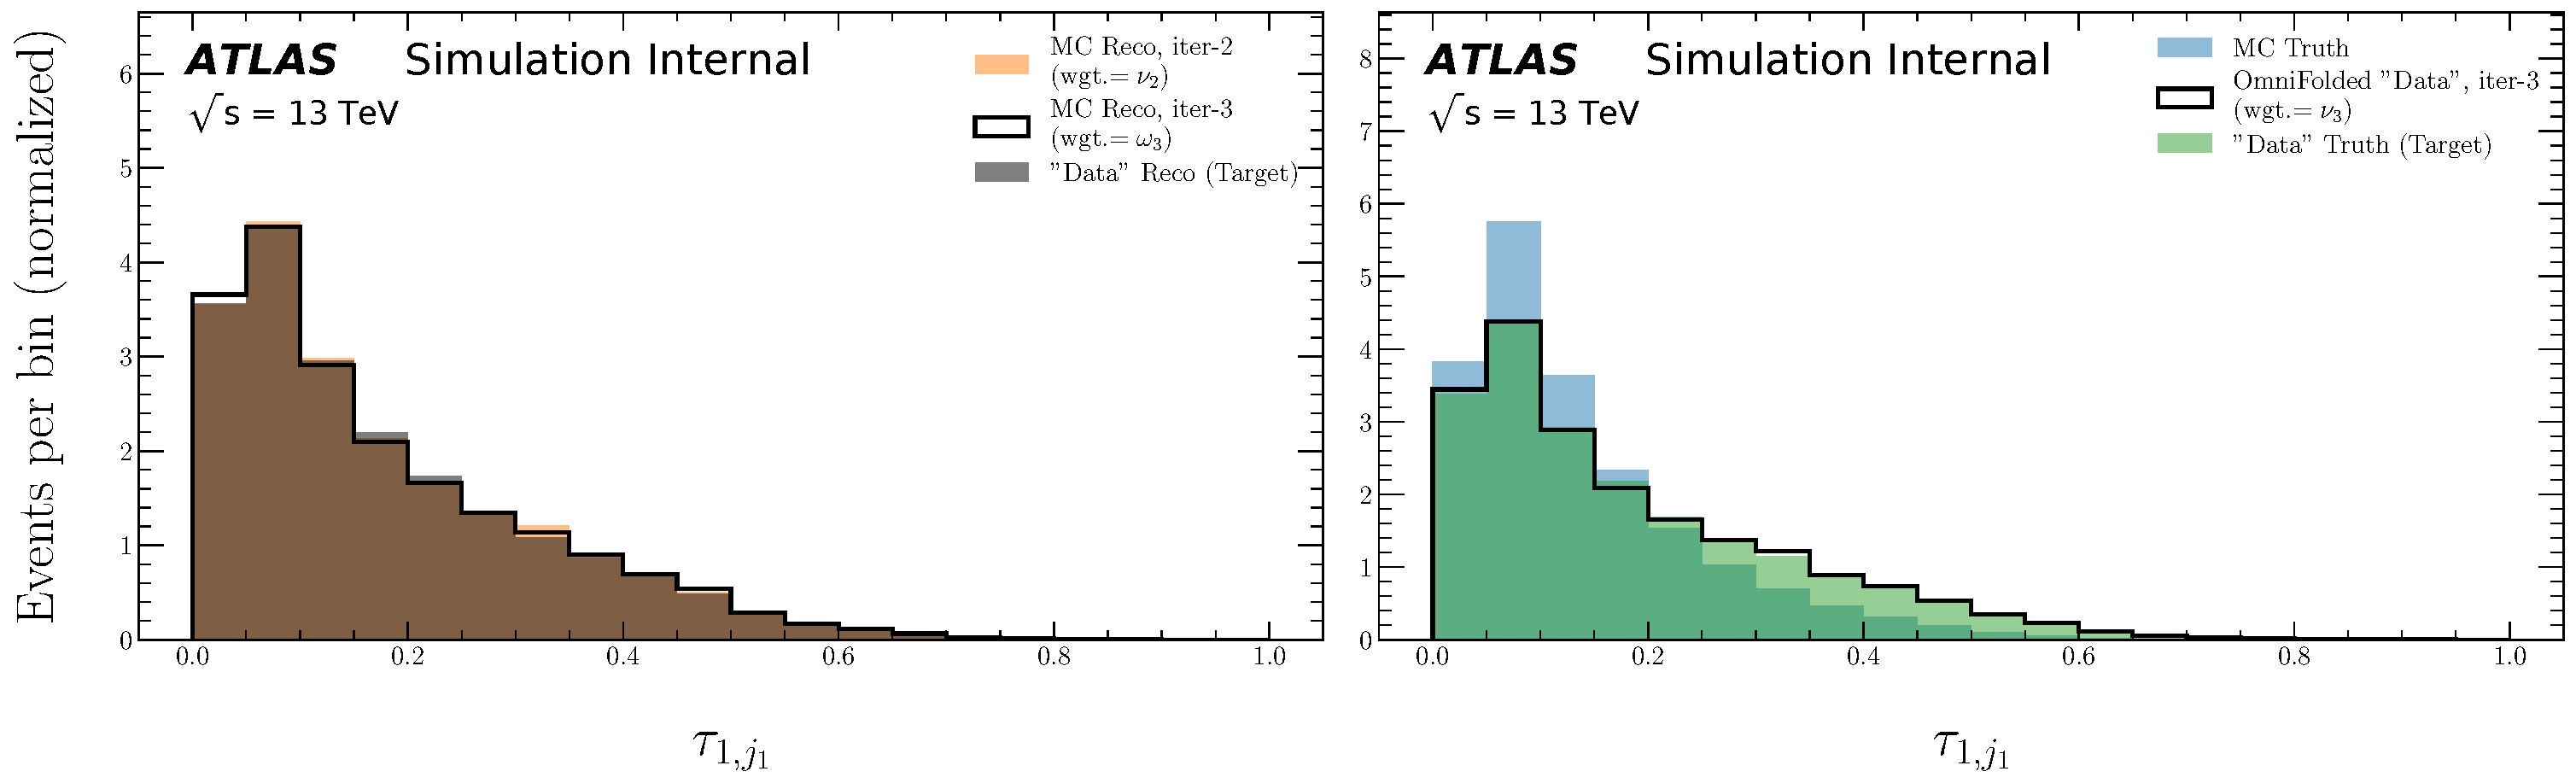
\includegraphics[width=0.85\textwidth]{figures/ATLASOmniFold-StressTest/ATLASOmniFold-StressTestA/MultiFold/tau1_trackj1/ATLASOmniFold-StressTestA-MultiFold-tau1_trackj1-Iteration03}}\\
\subfloat[After 4 iterations]{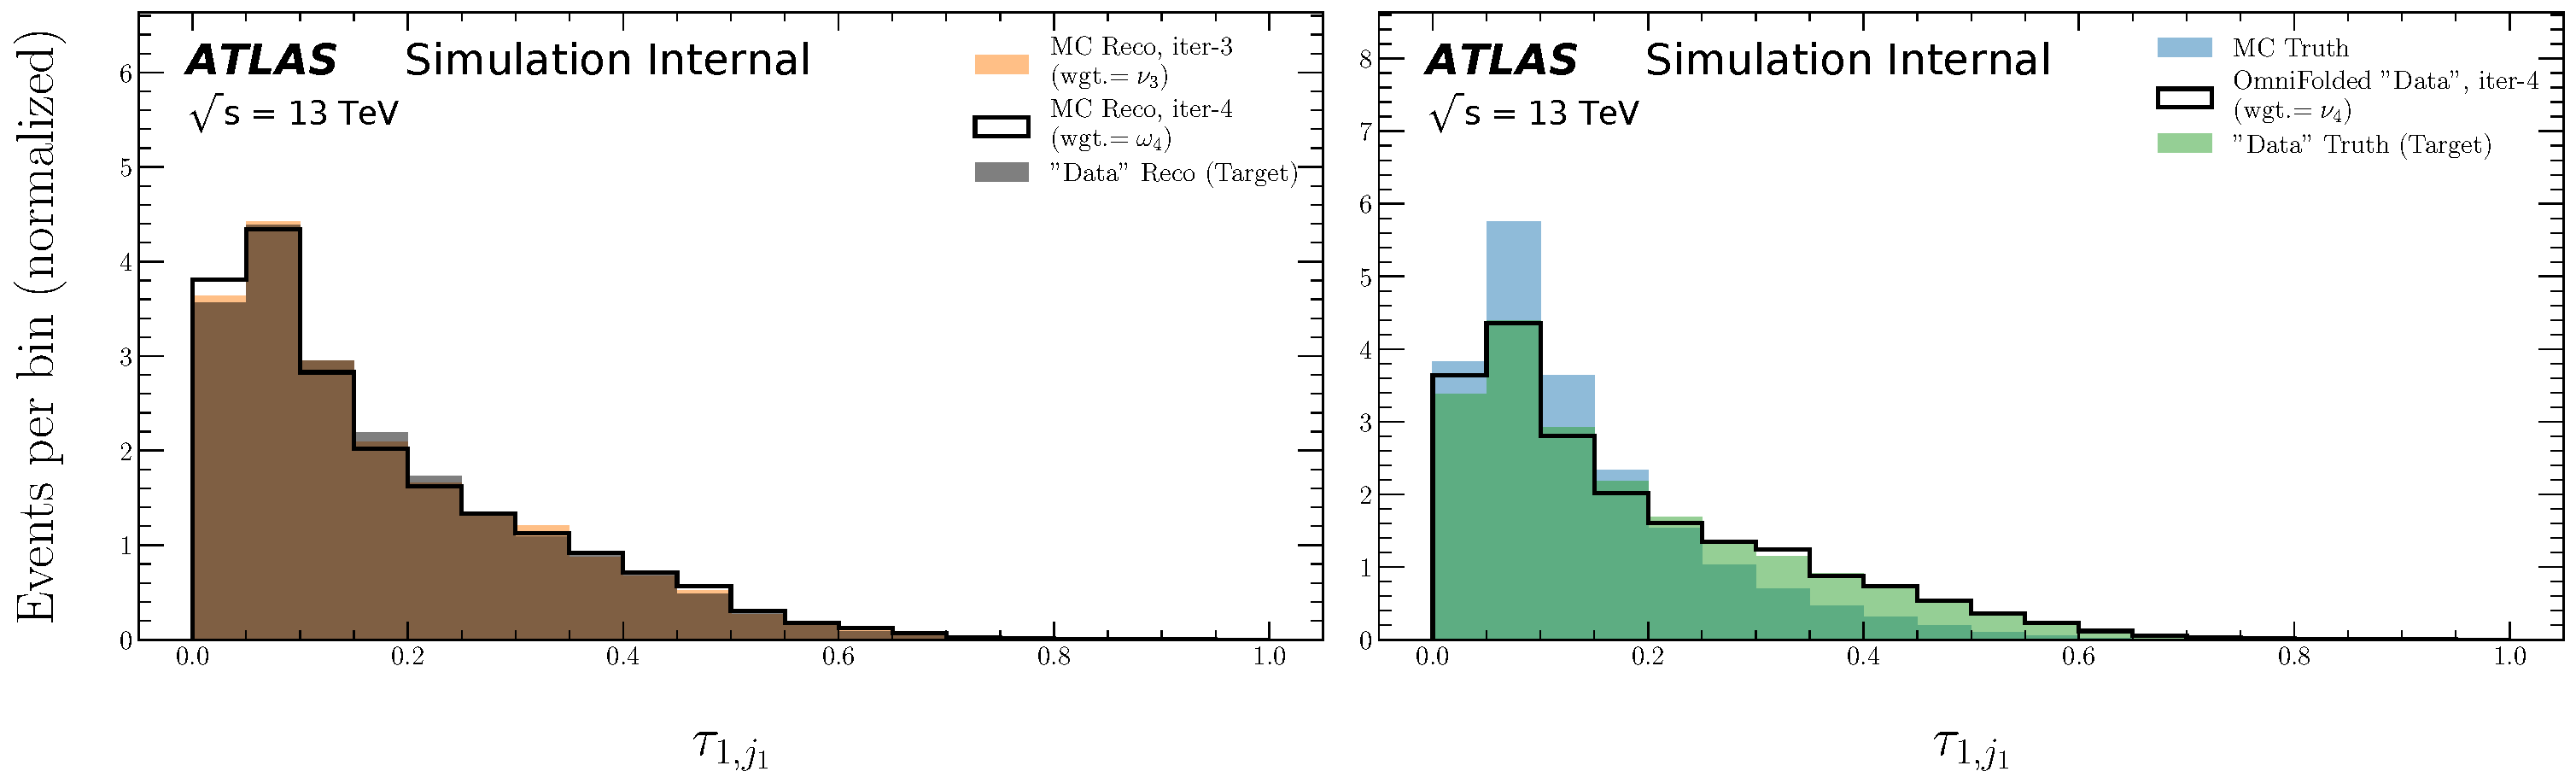
\includegraphics[width=0.85\textwidth]{figures/ATLASOmniFold-StressTest/ATLASOmniFold-StressTestA/MultiFold/tau1_trackj1/ATLASOmniFold-StressTestA-MultiFold-tau1_trackj1-Iteration04}}\\
\subfloat[After 5 iterations]{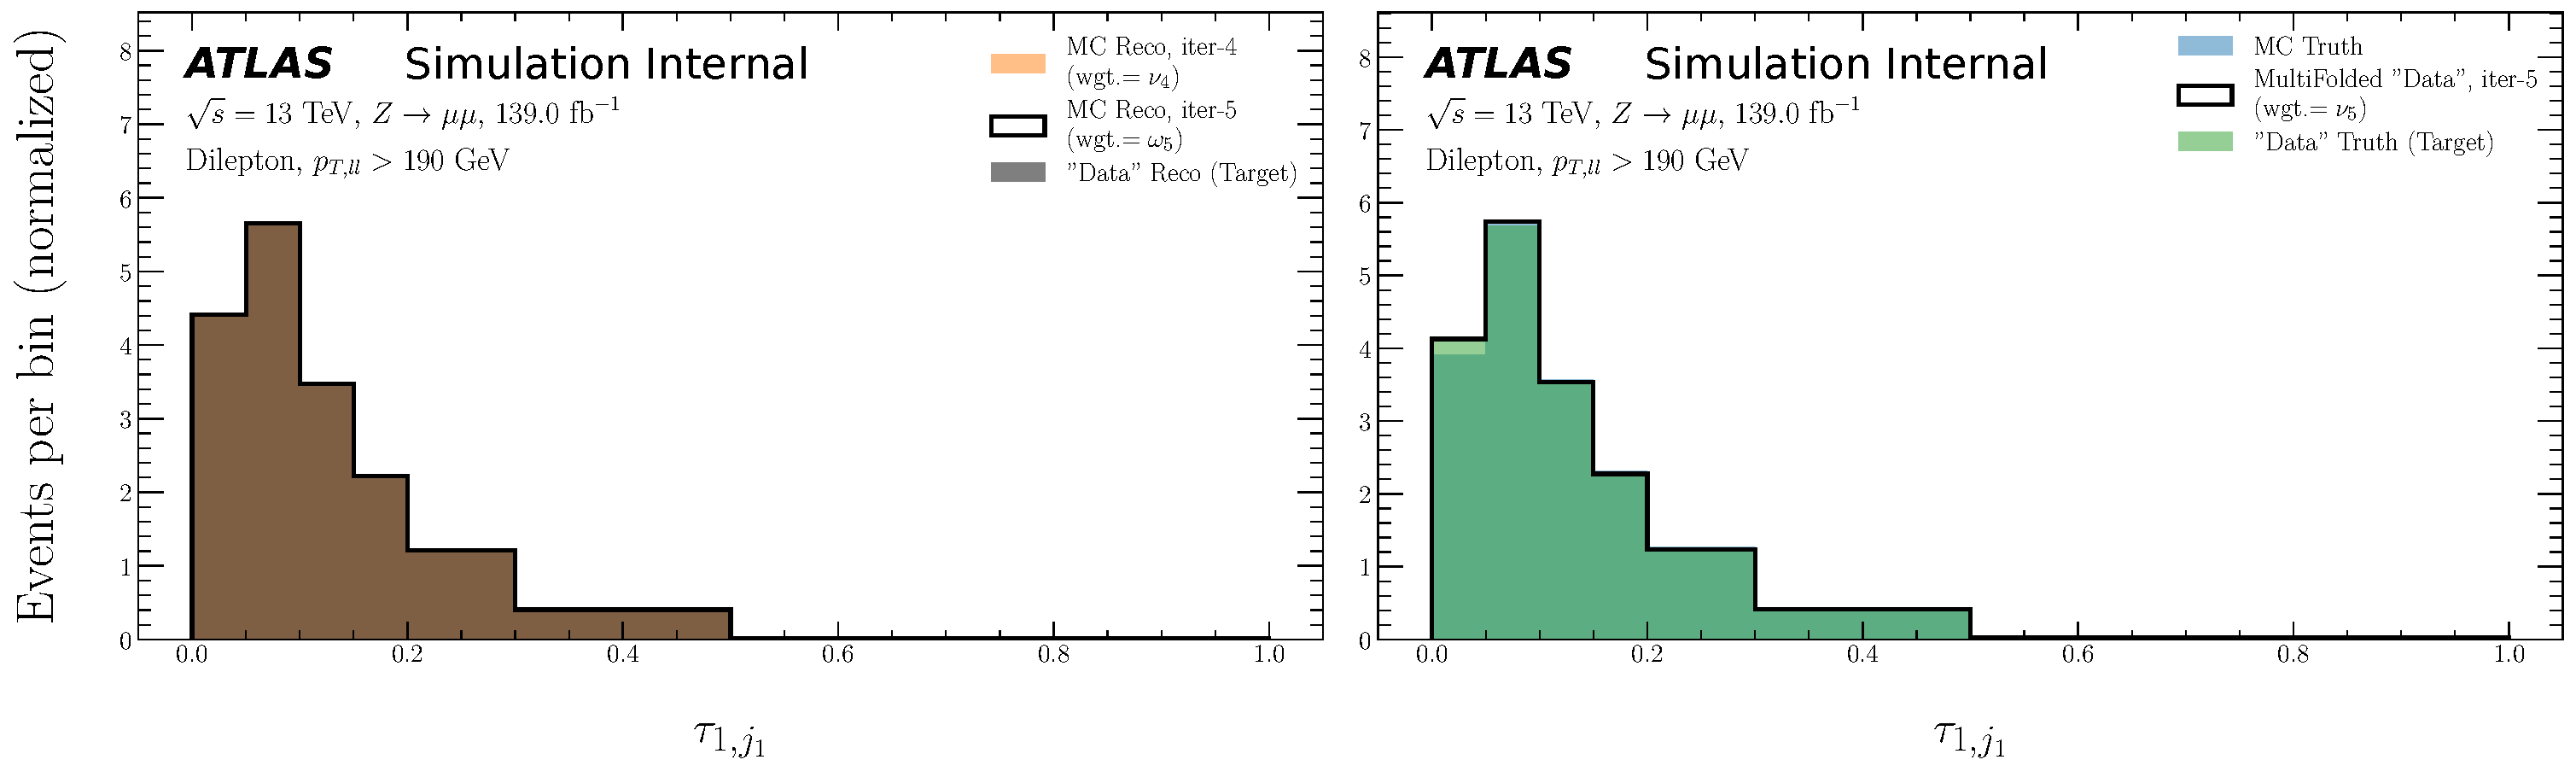
\includegraphics[width=0.85\textwidth]{figures/ATLASOmniFold-StressTest/ATLASOmniFold-StressTestA/MultiFold/tau1_trackj1/ATLASOmniFold-StressTestA-MultiFold-tau1_trackj1-Iteration05}}\\
\subfloat[After 6 iterations]{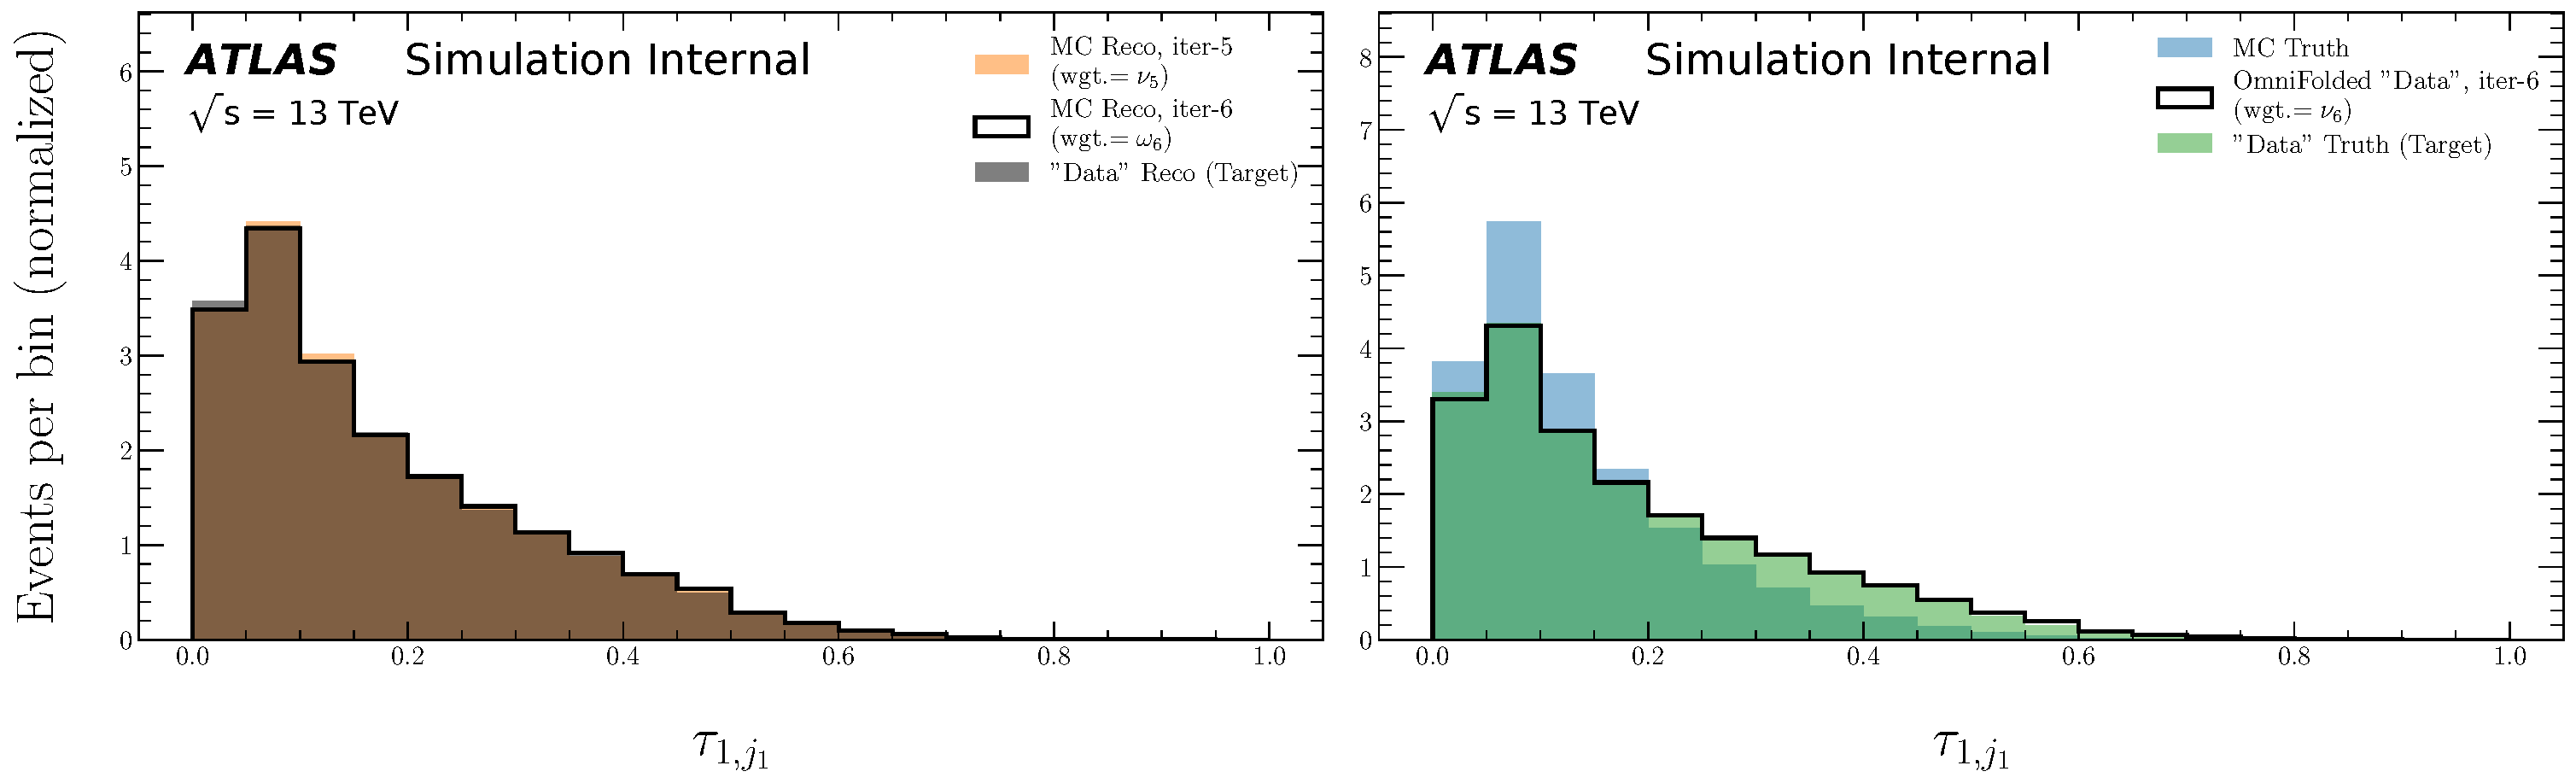
\includegraphics[width=0.85\textwidth]{figures/ATLASOmniFold-StressTest/ATLASOmniFold-StressTestA/MultiFold/tau1_trackj1/ATLASOmniFold-StressTestA-MultiFold-tau1_trackj1-Iteration06}}
\caption{A stress test for MultiFold using deterministic weights applied to the leading track jet $\tau_1$.}
\label{fig:stressa_tau1_trackj1Multi}
\end{figure}

\begin{figure}[h!]
\centering
\subfloat[Input histograms]{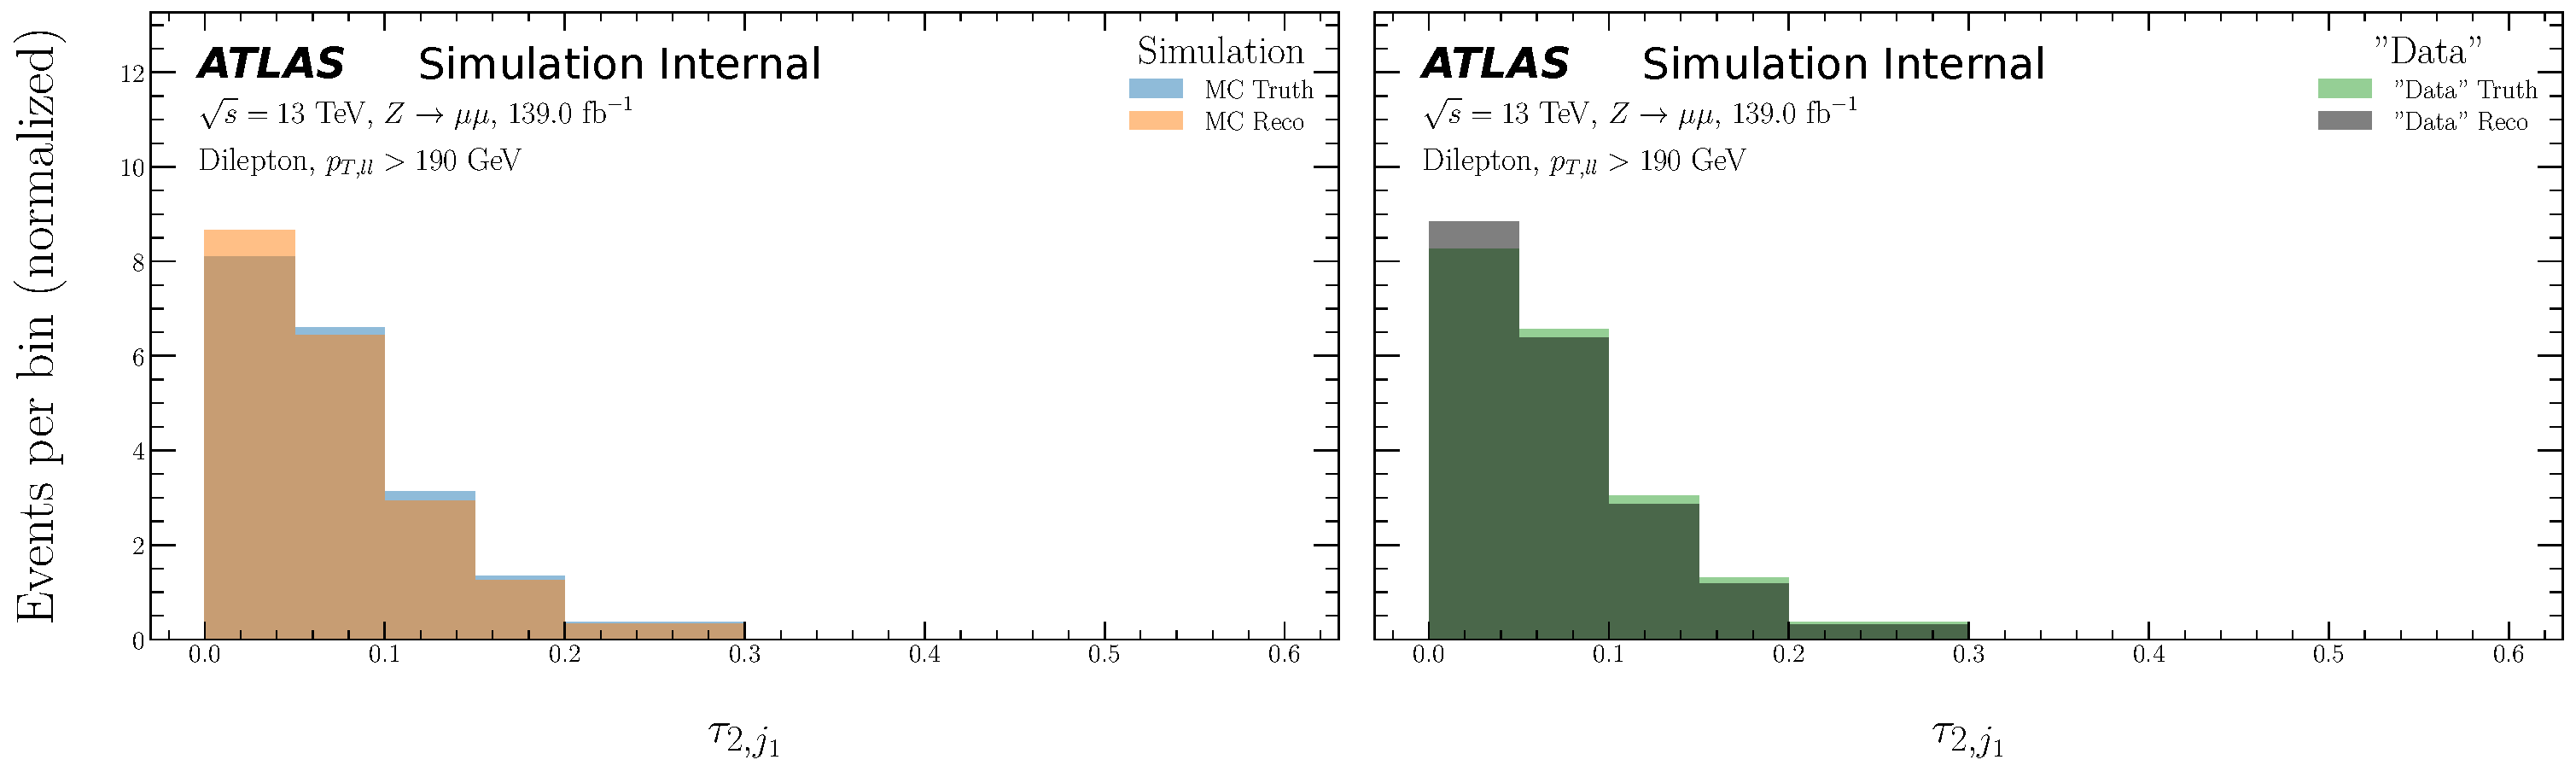
\includegraphics[width=0.85\textwidth]{figures/ATLASOmniFold-StressTest/ATLASOmniFold-StressTestA/MultiFold/tau2_trackj1/ATLASOmniFold-StressTestA-MultiFold-tau2_trackj1-Distributions}}\\
\subfloat[After 1 iteration]{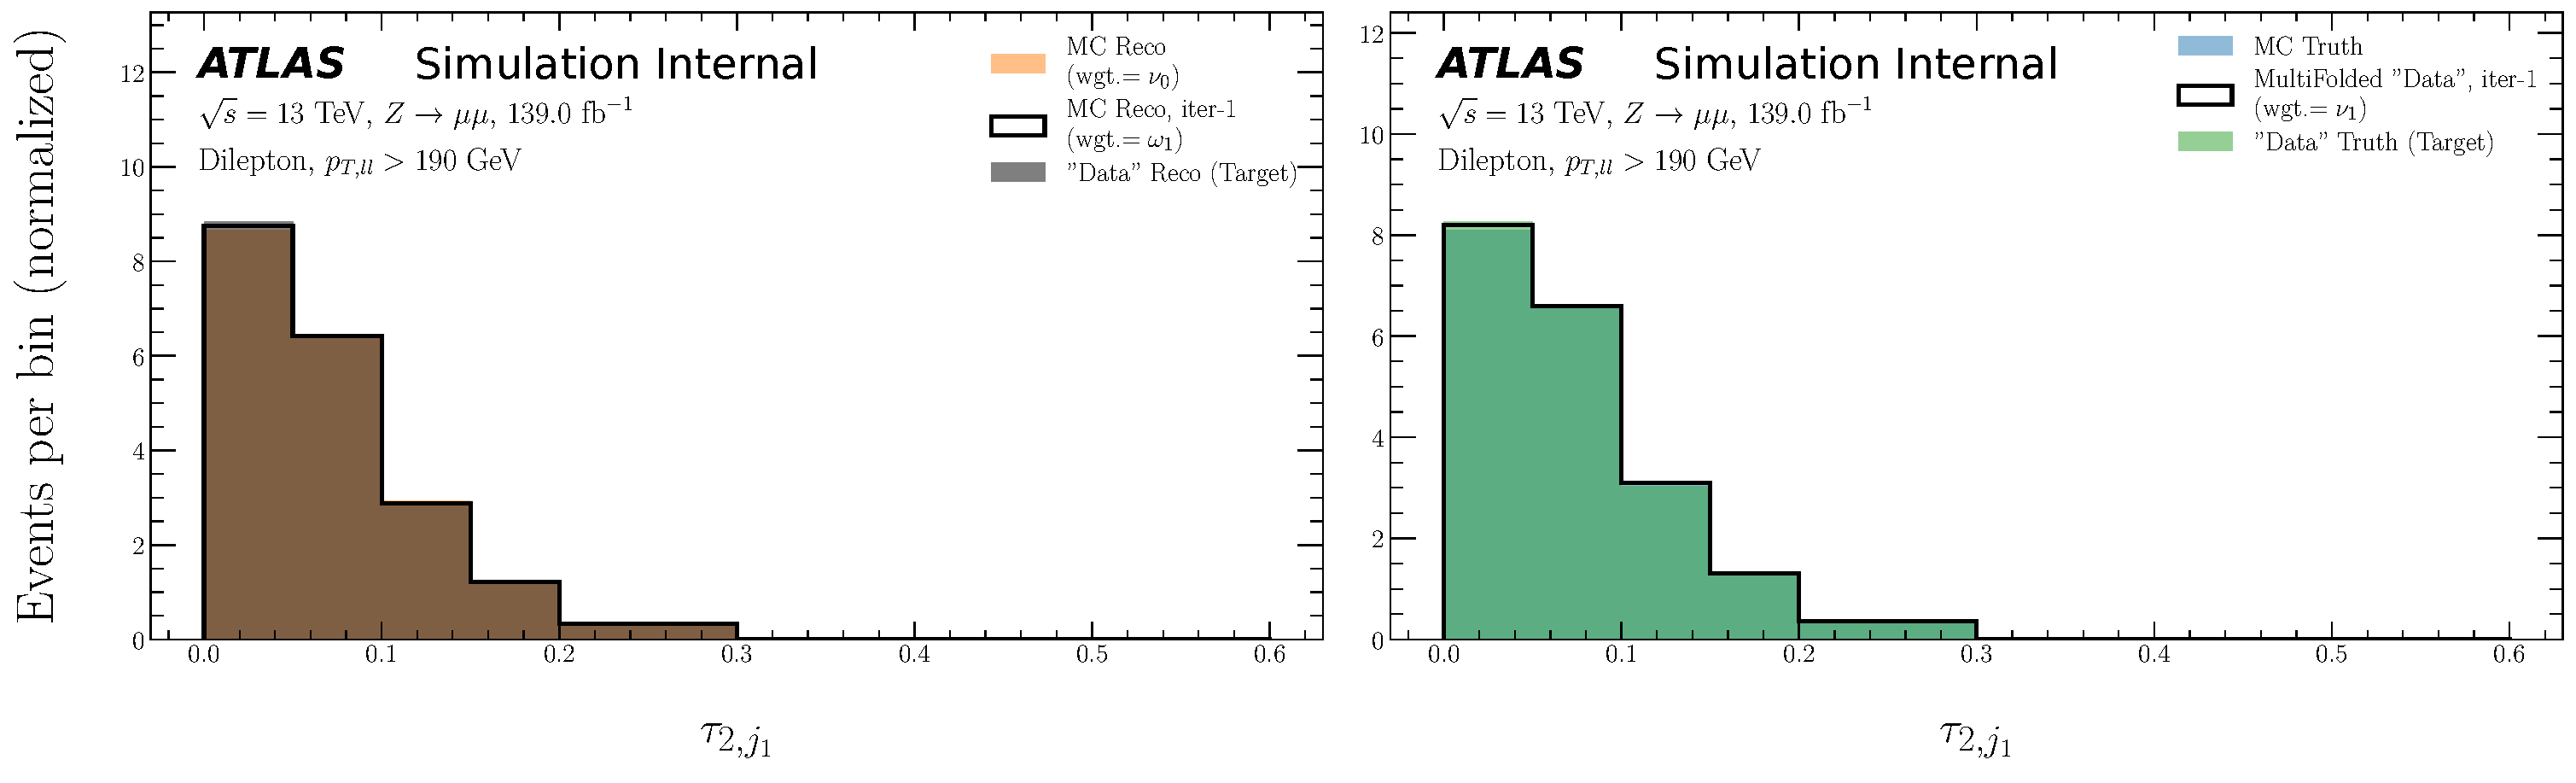
\includegraphics[width=0.85\textwidth]{figures/ATLASOmniFold-StressTest/ATLASOmniFold-StressTestA/MultiFold/tau2_trackj1/ATLASOmniFold-StressTestA-MultiFold-tau2_trackj1-Iteration01}}\\
\subfloat[After 2 iterations]{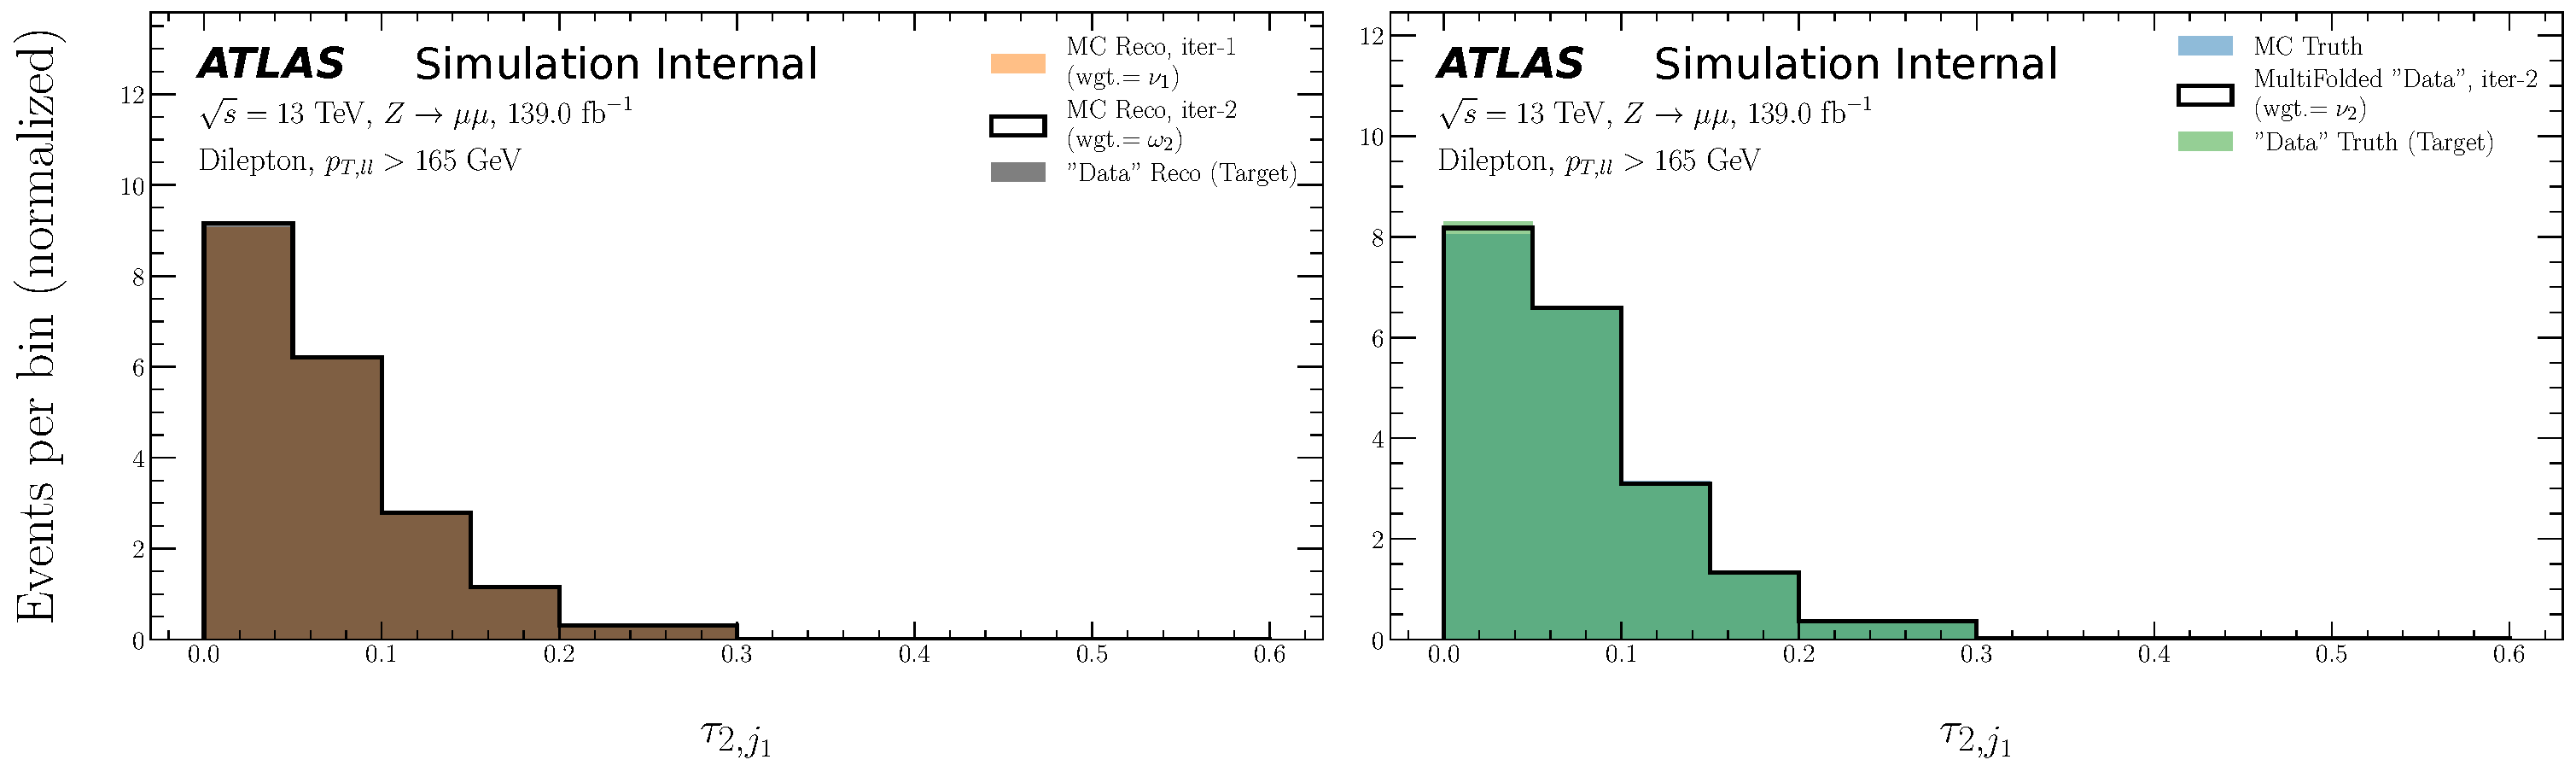
\includegraphics[width=0.85\textwidth]{figures/ATLASOmniFold-StressTest/ATLASOmniFold-StressTestA/MultiFold/tau2_trackj1/ATLASOmniFold-StressTestA-MultiFold-tau2_trackj1-Iteration02}}
\phantomcaption 
\end{figure}

\begin{figure}[h!]
\centering
\ContinuedFloat
\subfloat[After 3 iterations]{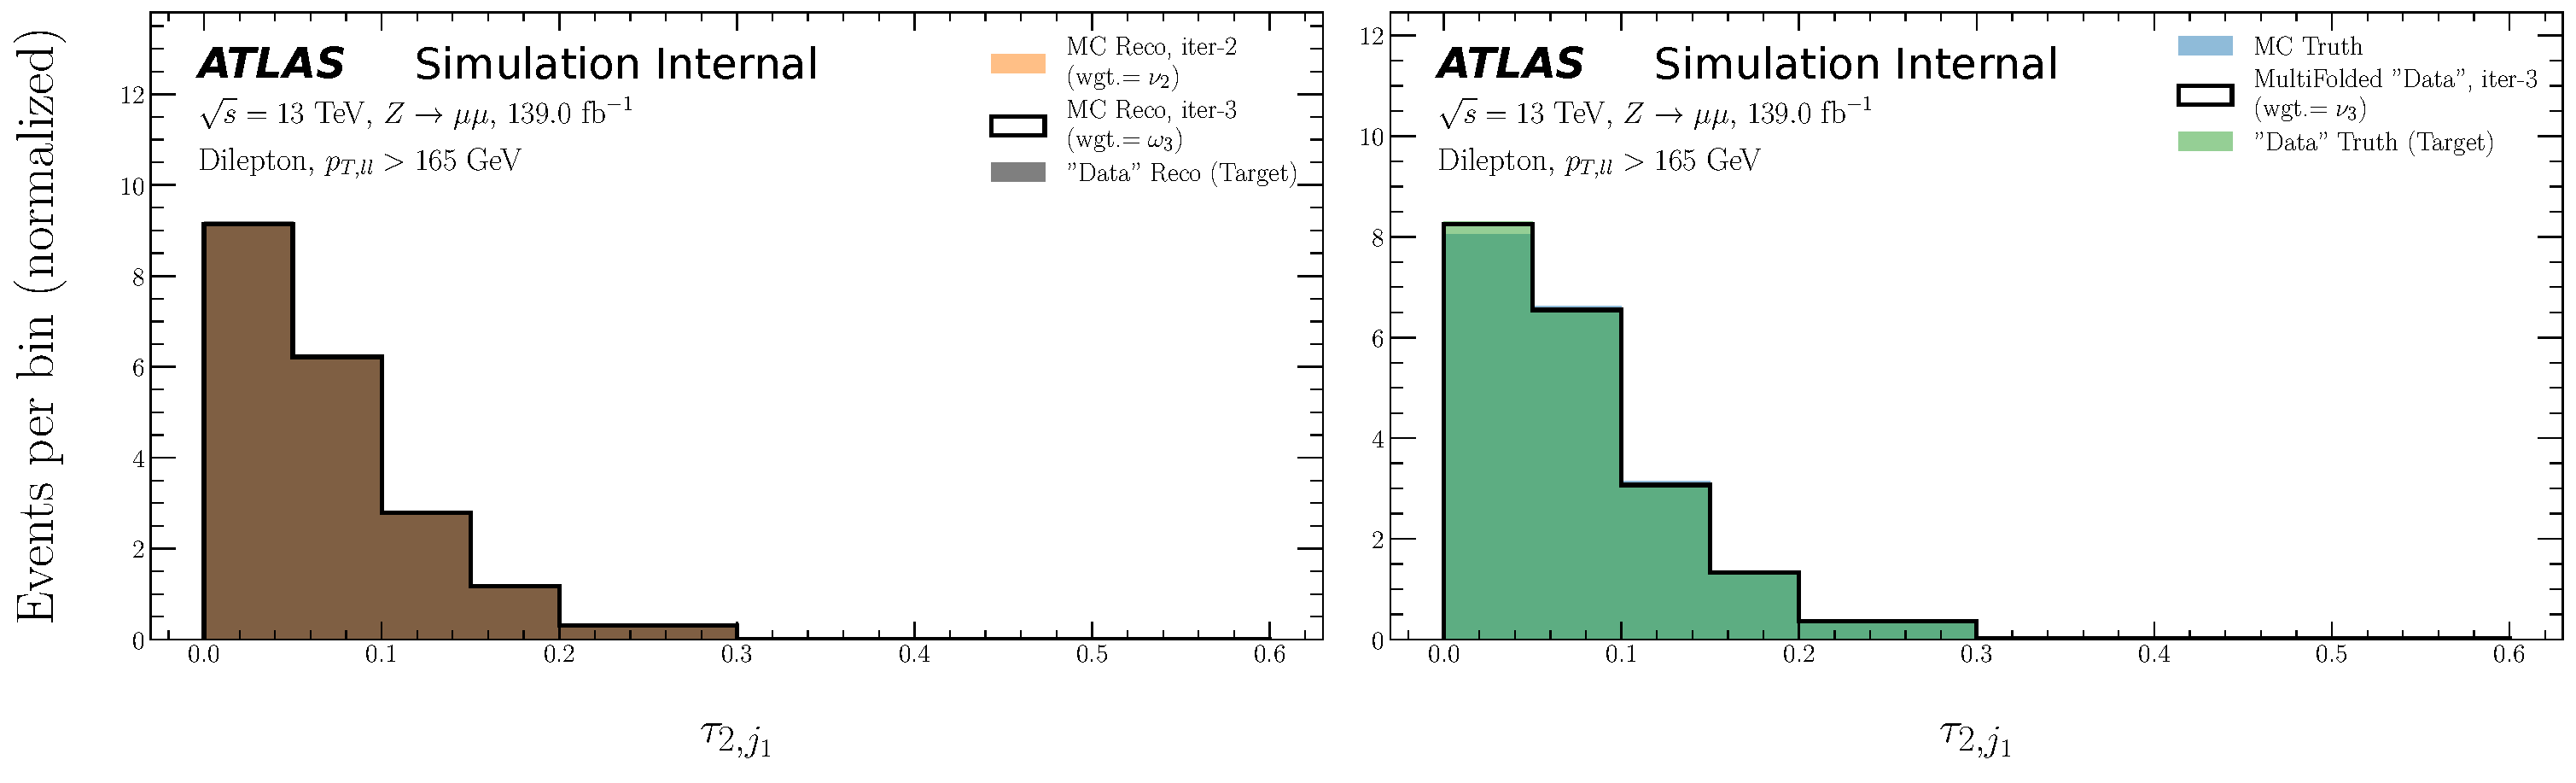
\includegraphics[width=0.85\textwidth]{figures/ATLASOmniFold-StressTest/ATLASOmniFold-StressTestA/MultiFold/tau2_trackj1/ATLASOmniFold-StressTestA-MultiFold-tau2_trackj1-Iteration03}}\\
\subfloat[After 4 iterations]{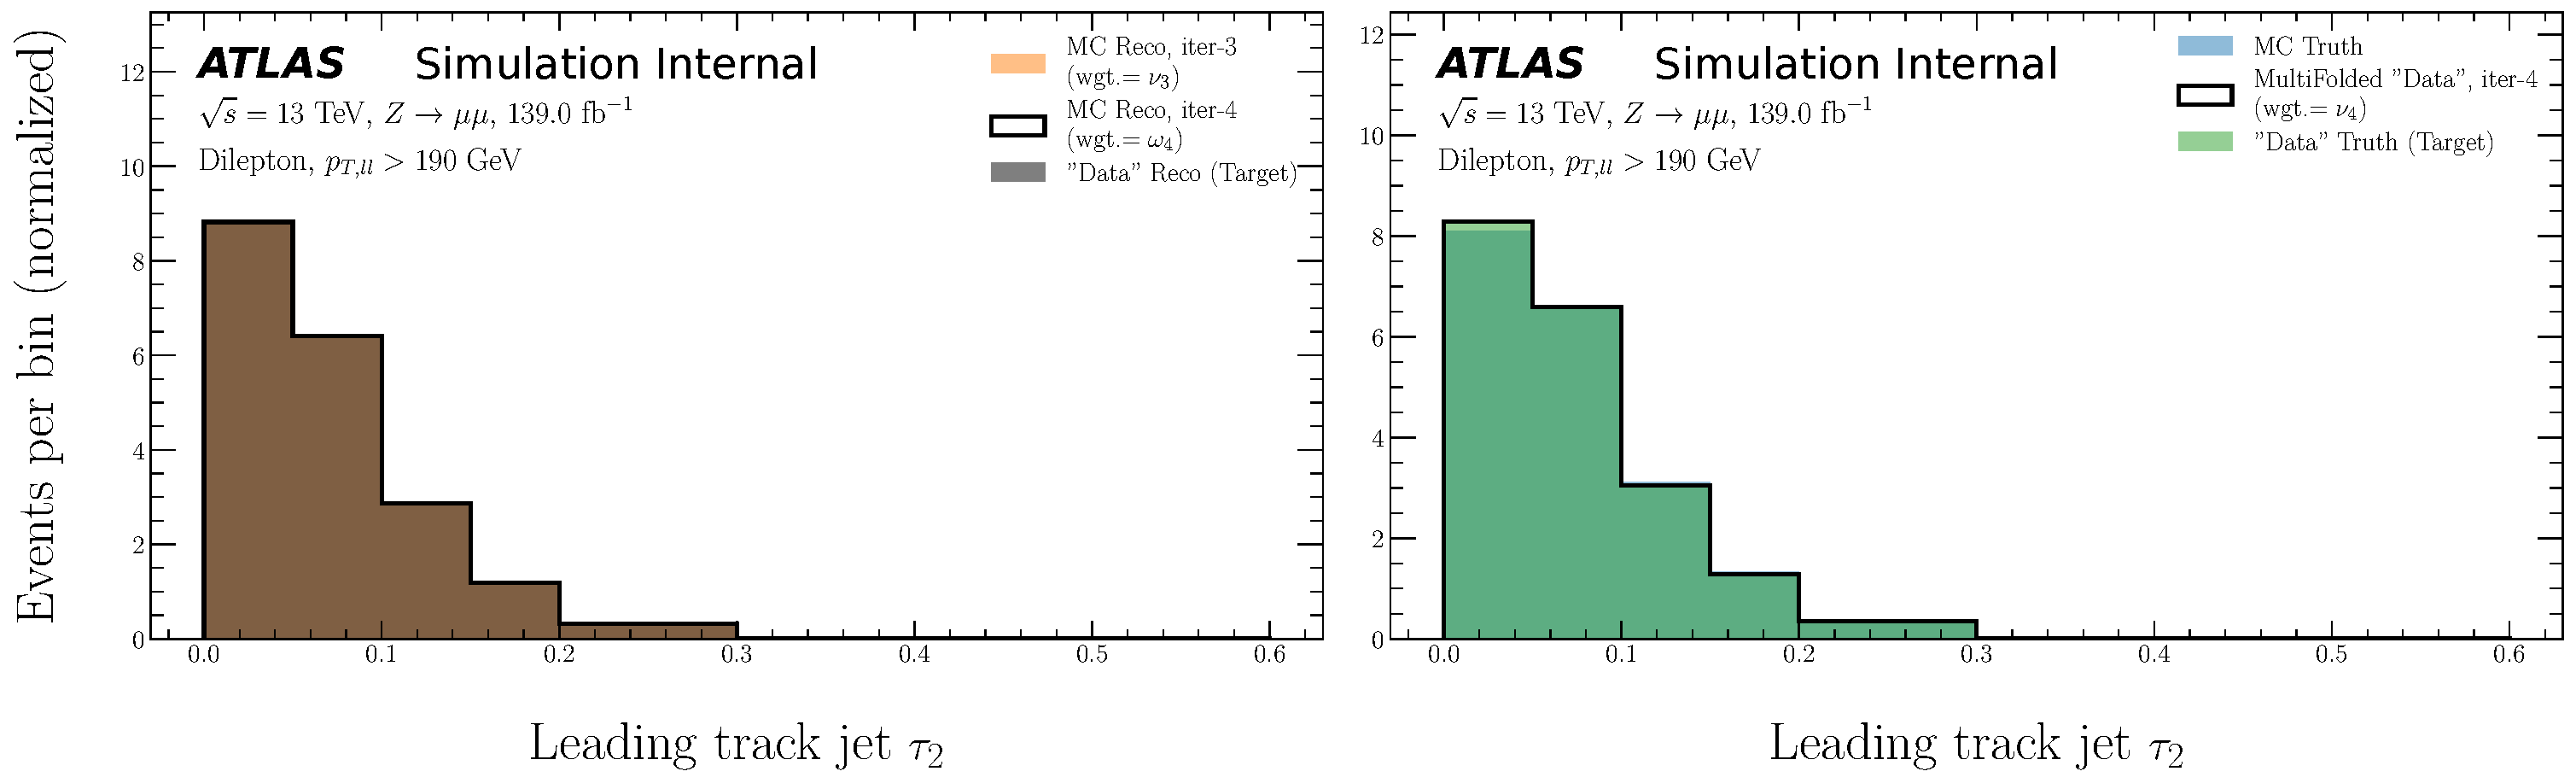
\includegraphics[width=0.85\textwidth]{figures/ATLASOmniFold-StressTest/ATLASOmniFold-StressTestA/MultiFold/tau2_trackj1/ATLASOmniFold-StressTestA-MultiFold-tau2_trackj1-Iteration04}}\\
\subfloat[After 5 iterations]{\includegraphics[width=0.85\textwidth]{figures/ATLASOmniFold-StressTest/ATLASOmniFold-StressTestA/MultiFold/tau2_trackj1/ATLASOmniFold-StressTestA-MultiFold-tau2_trackj1-Iteration05}}\\
\subfloat[After 6 iterations]{\includegraphics[width=0.85\textwidth]{figures/ATLASOmniFold-StressTest/ATLASOmniFold-StressTestA/MultiFold/tau2_trackj1/ATLASOmniFold-StressTestA-MultiFold-tau2_trackj1-Iteration06}}
\caption{A stress test for MultiFold using deterministic weights applied to the leading track jet $\tau_2$.}
\label{fig:stressa_tau2_trackj1Multi}
\end{figure}

\begin{figure}[h!]
\centering
\subfloat[Input histograms]{\includegraphics[width=0.85\textwidth]{figures/ATLASOmniFold-StressTest/ATLASOmniFold-StressTestA/MultiFold/tau3_trackj1/ATLASOmniFold-StressTestA-MultiFold-tau3_trackj1-Distributions}}\\
\subfloat[After 1 iteration]{\includegraphics[width=0.85\textwidth]{figures/ATLASOmniFold-StressTest/ATLASOmniFold-StressTestA/MultiFold/tau3_trackj1/ATLASOmniFold-StressTestA-MultiFold-tau3_trackj1-Iteration01}}\\
\subfloat[After 2 iterations]{\includegraphics[width=0.85\textwidth]{figures/ATLASOmniFold-StressTest/ATLASOmniFold-StressTestA/MultiFold/tau3_trackj1/ATLASOmniFold-StressTestA-MultiFold-tau3_trackj1-Iteration02}}
\phantomcaption 
\end{figure}

\begin{figure}[h!]
\centering
\ContinuedFloat
\subfloat[After 3 iterations]{\includegraphics[width=0.85\textwidth]{figures/ATLASOmniFold-StressTest/ATLASOmniFold-StressTestA/MultiFold/tau3_trackj1/ATLASOmniFold-StressTestA-MultiFold-tau3_trackj1-Iteration03}}\\
\subfloat[After 4 iterations]{\includegraphics[width=0.85\textwidth]{figures/ATLASOmniFold-StressTest/ATLASOmniFold-StressTestA/MultiFold/tau3_trackj1/ATLASOmniFold-StressTestA-MultiFold-tau3_trackj1-Iteration04}}\\
\subfloat[After 5 iterations]{\includegraphics[width=0.85\textwidth]{figures/ATLASOmniFold-StressTest/ATLASOmniFold-StressTestA/MultiFold/tau3_trackj1/ATLASOmniFold-StressTestA-MultiFold-tau3_trackj1-Iteration05}}\\
\subfloat[After 6 iterations]{\includegraphics[width=0.85\textwidth]{figures/ATLASOmniFold-StressTest/ATLASOmniFold-StressTestA/MultiFold/tau3_trackj1/ATLASOmniFold-StressTestA-MultiFold-tau3_trackj1-Iteration06}}
\caption{A stress test for MultiFold using deterministic weights applied to the leading track jet $\tau_3$.}
\label{fig:stressa_tau3_trackj1Multi}
\end{figure}

%%%

\begin{figure}[h!]
\centering
\subfloat[Input histograms]{\includegraphics[width=0.85\textwidth]{figures/ATLASOmniFold-StressTest/ATLASOmniFold-StressTestA/MultiFold/m_trackj2/ATLASOmniFold-StressTestA-MultiFold-m_trackj2-Distributions}}\\
\subfloat[After 1 iteration]{\includegraphics[width=0.85\textwidth]{figures/ATLASOmniFold-StressTest/ATLASOmniFold-StressTestA/MultiFold/m_trackj2/ATLASOmniFold-StressTestA-MultiFold-m_trackj2-Iteration01}}\\
\subfloat[After 2 iterations]{\includegraphics[width=0.85\textwidth]{figures/ATLASOmniFold-StressTest/ATLASOmniFold-StressTestA/MultiFold/m_trackj2/ATLASOmniFold-StressTestA-MultiFold-m_trackj2-Iteration02}}
\phantomcaption 
\end{figure}

\begin{figure}[h!]
\centering
\ContinuedFloat
\subfloat[After 3 iterations]{\includegraphics[width=0.85\textwidth]{figures/ATLASOmniFold-StressTest/ATLASOmniFold-StressTestA/MultiFold/m_trackj2/ATLASOmniFold-StressTestA-MultiFold-m_trackj2-Iteration03}}\\
\subfloat[After 4 iterations]{\includegraphics[width=0.85\textwidth]{figures/ATLASOmniFold-StressTest/ATLASOmniFold-StressTestA/MultiFold/m_trackj2/ATLASOmniFold-StressTestA-MultiFold-m_trackj2-Iteration04}}\\
\subfloat[After 5 iterations]{\includegraphics[width=0.85\textwidth]{figures/ATLASOmniFold-StressTest/ATLASOmniFold-StressTestA/MultiFold/m_trackj2/ATLASOmniFold-StressTestA-MultiFold-m_trackj2-Iteration05}}\\
\subfloat[After 6 iterations]{\includegraphics[width=0.85\textwidth]{figures/ATLASOmniFold-StressTest/ATLASOmniFold-StressTestA/MultiFold/m_trackj2/ATLASOmniFold-StressTestA-MultiFold-m_trackj2-Iteration06}}
\caption{A stress test for MultiFold using deterministic weights applied to the subleading track jet mass.}
\label{fig:stressa_massMulti}
\end{figure}

\begin{figure}[h!]
\centering
\subfloat[Input histograms]{\includegraphics[width=0.85\textwidth]{figures/ATLASOmniFold-StressTest/ATLASOmniFold-StressTestA/MultiFold/Ntracks_trackj2/ATLASOmniFold-StressTestA-MultiFold-Ntracks_trackj2-Distributions}}\\
\subfloat[After 1 iteration]{\includegraphics[width=0.85\textwidth]{figures/ATLASOmniFold-StressTest/ATLASOmniFold-StressTestA/MultiFold/Ntracks_trackj2/ATLASOmniFold-StressTestA-MultiFold-Ntracks_trackj2-Iteration01}}\\
\subfloat[After 2 iterations]{\includegraphics[width=0.85\textwidth]{figures/ATLASOmniFold-StressTest/ATLASOmniFold-StressTestA/MultiFold/Ntracks_trackj2/ATLASOmniFold-StressTestA-MultiFold-Ntracks_trackj2-Iteration02}}
\phantomcaption 
\end{figure}

\begin{figure}[h!]
\centering
\ContinuedFloat
\subfloat[After 3 iterations]{\includegraphics[width=0.85\textwidth]{figures/ATLASOmniFold-StressTest/ATLASOmniFold-StressTestA/MultiFold/Ntracks_trackj2/ATLASOmniFold-StressTestA-MultiFold-Ntracks_trackj2-Iteration03}}\\
\subfloat[After 4 iterations]{\includegraphics[width=0.85\textwidth]{figures/ATLASOmniFold-StressTest/ATLASOmniFold-StressTestA/MultiFold/Ntracks_trackj2/ATLASOmniFold-StressTestA-MultiFold-Ntracks_trackj2-Iteration04}}\\
\subfloat[After 5 iterations]{\includegraphics[width=0.85\textwidth]{figures/ATLASOmniFold-StressTest/ATLASOmniFold-StressTestA/MultiFold/Ntracks_trackj2/ATLASOmniFold-StressTestA-MultiFold-Ntracks_trackj2-Iteration05}}\\
\subfloat[After 6 iterations]{\includegraphics[width=0.85\textwidth]{figures/ATLASOmniFold-StressTest/ATLASOmniFold-StressTestA/MultiFold/Ntracks_trackj2/ATLASOmniFold-StressTestA-MultiFold-Ntracks_trackj2-Iteration06}}
\caption{A stress test for MultiFold using deterministic weights applied to the subleading track jet constituent multiplicity.}
\label{fig:stressa_Ntracks_trackj2Multi}
\end{figure}


%%%

\begin{figure}[h!]
\centering
\subfloat[Input histograms]{\includegraphics[width=0.85\textwidth]{figures/ATLASOmniFold-StressTest/ATLASOmniFold-StressTestA/MultiFold/pT_trackj2/ATLASOmniFold-StressTestA-MultiFold-pT_trackj2-Distributions}}\\
\subfloat[After 1 iteration]{\includegraphics[width=0.85\textwidth]{figures/ATLASOmniFold-StressTest/ATLASOmniFold-StressTestA/MultiFold/pT_trackj2/ATLASOmniFold-StressTestA-MultiFold-pT_trackj2-Iteration01}}\\
\subfloat[After 2 iterations]{\includegraphics[width=0.85\textwidth]{figures/ATLASOmniFold-StressTest/ATLASOmniFold-StressTestA/MultiFold/pT_trackj2/ATLASOmniFold-StressTestA-MultiFold-pT_trackj2-Iteration02}}
\phantomcaption 
\end{figure}

\begin{figure}[h!]
\centering
\ContinuedFloat
\subfloat[After 3 iterations]{\includegraphics[width=0.85\textwidth]{figures/ATLASOmniFold-StressTest/ATLASOmniFold-StressTestA/MultiFold/pT_trackj2/ATLASOmniFold-StressTestA-MultiFold-pT_trackj2-Iteration03}}\\
\subfloat[After 4 iterations]{\includegraphics[width=0.85\textwidth]{figures/ATLASOmniFold-StressTest/ATLASOmniFold-StressTestA/MultiFold/pT_trackj2/ATLASOmniFold-StressTestA-MultiFold-pT_trackj2-Iteration04}}\\
\subfloat[After 5 iterations]{\includegraphics[width=0.85\textwidth]{figures/ATLASOmniFold-StressTest/ATLASOmniFold-StressTestA/MultiFold/pT_trackj2/ATLASOmniFold-StressTestA-MultiFold-pT_trackj2-Iteration05}}\\
\subfloat[After 6 iterations]{\includegraphics[width=0.85\textwidth]{figures/ATLASOmniFold-StressTest/ATLASOmniFold-StressTestA/MultiFold/pT_trackj2/ATLASOmniFold-StressTestA-MultiFold-pT_trackj2-Iteration06}}
\caption{A stress test for MultiFold using deterministic weights applied to the subleading track jet $p_T$.}
\label{fig:stressa_pT_trackj2Multi}
\end{figure}

\begin{figure}[h!]
\centering
\subfloat[Input histograms]{\includegraphics[width=0.85\textwidth]{figures/ATLASOmniFold-StressTest/ATLASOmniFold-StressTestA/MultiFold/y_trackj2/ATLASOmniFold-StressTestA-MultiFold-y_trackj2-Distributions}}\\
\subfloat[After 1 iteration]{\includegraphics[width=0.85\textwidth]{figures/ATLASOmniFold-StressTest/ATLASOmniFold-StressTestA/MultiFold/y_trackj2/ATLASOmniFold-StressTestA-MultiFold-y_trackj2-Iteration01}}\\
\subfloat[After 2 iterations]{\includegraphics[width=0.85\textwidth]{figures/ATLASOmniFold-StressTest/ATLASOmniFold-StressTestA/MultiFold/y_trackj2/ATLASOmniFold-StressTestA-MultiFold-y_trackj2-Iteration02}}
\phantomcaption 
\end{figure}

\begin{figure}[h!]
\centering
\ContinuedFloat
\subfloat[After 3 iterations]{\includegraphics[width=0.85\textwidth]{figures/ATLASOmniFold-StressTest/ATLASOmniFold-StressTestA/MultiFold/y_trackj2/ATLASOmniFold-StressTestA-MultiFold-y_trackj2-Iteration03}}\\
\subfloat[After 4 iterations]{\includegraphics[width=0.85\textwidth]{figures/ATLASOmniFold-StressTest/ATLASOmniFold-StressTestA/MultiFold/y_trackj2/ATLASOmniFold-StressTestA-MultiFold-y_trackj2-Iteration04}}\\
\subfloat[After 5 iterations]{\includegraphics[width=0.85\textwidth]{figures/ATLASOmniFold-StressTest/ATLASOmniFold-StressTestA/MultiFold/y_trackj2/ATLASOmniFold-StressTestA-MultiFold-y_trackj2-Iteration05}}\\
\subfloat[After 6 iterations]{\includegraphics[width=0.85\textwidth]{figures/ATLASOmniFold-StressTest/ATLASOmniFold-StressTestA/MultiFold/y_trackj2/ATLASOmniFold-StressTestA-MultiFold-y_trackj2-Iteration06}}
\caption{A stress test for MultiFold using deterministic weights applied to the subleading track jet rapidity.}
\label{fig:stressa_y_trackj2Multi}
\end{figure}

\begin{figure}[h!]
\centering
\subfloat[Input histograms]{\includegraphics[width=0.85\textwidth]{figures/ATLASOmniFold-StressTest/ATLASOmniFold-StressTestA/MultiFold/tau1_trackj2/ATLASOmniFold-StressTestA-MultiFold-tau1_trackj2-Distributions}}\\
\subfloat[After 1 iteration]{\includegraphics[width=0.85\textwidth]{figures/ATLASOmniFold-StressTest/ATLASOmniFold-StressTestA/MultiFold/tau1_trackj2/ATLASOmniFold-StressTestA-MultiFold-tau1_trackj2-Iteration01}}\\
\subfloat[After 2 iterations]{\includegraphics[width=0.85\textwidth]{figures/ATLASOmniFold-StressTest/ATLASOmniFold-StressTestA/MultiFold/tau1_trackj2/ATLASOmniFold-StressTestA-MultiFold-tau1_trackj2-Iteration02}}
\phantomcaption 
\end{figure}

\begin{figure}[h!]
\centering
\ContinuedFloat
\subfloat[After 3 iterations]{\includegraphics[width=0.85\textwidth]{figures/ATLASOmniFold-StressTest/ATLASOmniFold-StressTestA/MultiFold/tau1_trackj2/ATLASOmniFold-StressTestA-MultiFold-tau1_trackj2-Iteration03}}\\
\subfloat[After 4 iterations]{\includegraphics[width=0.85\textwidth]{figures/ATLASOmniFold-StressTest/ATLASOmniFold-StressTestA/MultiFold/tau1_trackj2/ATLASOmniFold-StressTestA-MultiFold-tau1_trackj2-Iteration04}}\\
\subfloat[After 5 iterations]{\includegraphics[width=0.85\textwidth]{figures/ATLASOmniFold-StressTest/ATLASOmniFold-StressTestA/MultiFold/tau1_trackj2/ATLASOmniFold-StressTestA-MultiFold-tau1_trackj2-Iteration05}}\\
\subfloat[After 6 iterations]{\includegraphics[width=0.85\textwidth]{figures/ATLASOmniFold-StressTest/ATLASOmniFold-StressTestA/MultiFold/tau1_trackj2/ATLASOmniFold-StressTestA-MultiFold-tau1_trackj2-Iteration06}}
\caption{A stress test for MultiFold using deterministic weights applied to the subleading track jet $\tau_1$.}
\label{fig:stressa_tau1_trackj2Multi}
\end{figure}

\begin{figure}[h!]
\centering
\subfloat[Input histograms]{\includegraphics[width=0.85\textwidth]{figures/ATLASOmniFold-StressTest/ATLASOmniFold-StressTestA/MultiFold/tau2_trackj2/ATLASOmniFold-StressTestA-MultiFold-tau2_trackj2-Distributions}}\\
\subfloat[After 1 iteration]{\includegraphics[width=0.85\textwidth]{figures/ATLASOmniFold-StressTest/ATLASOmniFold-StressTestA/MultiFold/tau2_trackj2/ATLASOmniFold-StressTestA-MultiFold-tau2_trackj2-Iteration01}}\\
\subfloat[After 2 iterations]{\includegraphics[width=0.85\textwidth]{figures/ATLASOmniFold-StressTest/ATLASOmniFold-StressTestA/MultiFold/tau2_trackj2/ATLASOmniFold-StressTestA-MultiFold-tau2_trackj2-Iteration02}}
\phantomcaption 
\end{figure}

\begin{figure}[h!]
\centering
\ContinuedFloat
\subfloat[After 3 iterations]{\includegraphics[width=0.85\textwidth]{figures/ATLASOmniFold-StressTest/ATLASOmniFold-StressTestA/MultiFold/tau2_trackj2/ATLASOmniFold-StressTestA-MultiFold-tau2_trackj2-Iteration03}}\\
\subfloat[After 4 iterations]{\includegraphics[width=0.85\textwidth]{figures/ATLASOmniFold-StressTest/ATLASOmniFold-StressTestA/MultiFold/tau2_trackj2/ATLASOmniFold-StressTestA-MultiFold-tau2_trackj2-Iteration04}}\\
\subfloat[After 5 iterations]{\includegraphics[width=0.85\textwidth]{figures/ATLASOmniFold-StressTest/ATLASOmniFold-StressTestA/MultiFold/tau2_trackj2/ATLASOmniFold-StressTestA-MultiFold-tau2_trackj2-Iteration05}}\\
\subfloat[After 6 iterations]{\includegraphics[width=0.85\textwidth]{figures/ATLASOmniFold-StressTest/ATLASOmniFold-StressTestA/MultiFold/tau2_trackj2/ATLASOmniFold-StressTestA-MultiFold-tau2_trackj2-Iteration06}}
\caption{A stress test for MultiFold using deterministic weights applied to the subleading track jet $\tau_2$.}
\label{fig:stressa_tau2_trackj2Multi}
\end{figure}

\begin{figure}[h!]
\centering
\subfloat[Input histograms]{\includegraphics[width=0.85\textwidth]{figures/ATLASOmniFold-StressTest/ATLASOmniFold-StressTestA/MultiFold/tau3_trackj2/ATLASOmniFold-StressTestA-MultiFold-tau3_trackj2-Distributions}}\\
\subfloat[After 1 iteration]{\includegraphics[width=0.85\textwidth]{figures/ATLASOmniFold-StressTest/ATLASOmniFold-StressTestA/MultiFold/tau3_trackj2/ATLASOmniFold-StressTestA-MultiFold-tau3_trackj2-Iteration01}}\\
\subfloat[After 2 iterations]{\includegraphics[width=0.85\textwidth]{figures/ATLASOmniFold-StressTest/ATLASOmniFold-StressTestA/MultiFold/tau3_trackj2/ATLASOmniFold-StressTestA-MultiFold-tau3_trackj2-Iteration02}}
\phantomcaption 
\end{figure}

\begin{figure}[h!]
\centering
\ContinuedFloat
\subfloat[After 3 iterations]{\includegraphics[width=0.85\textwidth]{figures/ATLASOmniFold-StressTest/ATLASOmniFold-StressTestA/MultiFold/tau3_trackj2/ATLASOmniFold-StressTestA-MultiFold-tau3_trackj2-Iteration03}}\\
\subfloat[After 4 iterations]{\includegraphics[width=0.85\textwidth]{figures/ATLASOmniFold-StressTest/ATLASOmniFold-StressTestA/MultiFold/tau3_trackj2/ATLASOmniFold-StressTestA-MultiFold-tau3_trackj2-Iteration04}}\\
\subfloat[After 5 iterations]{\includegraphics[width=0.85\textwidth]{figures/ATLASOmniFold-StressTest/ATLASOmniFold-StressTestA/MultiFold/tau3_trackj2/ATLASOmniFold-StressTestA-MultiFold-tau3_trackj2-Iteration05}}\\
\subfloat[After 6 iterations]{\includegraphics[width=0.85\textwidth]{figures/ATLASOmniFold-StressTest/ATLASOmniFold-StressTestA/MultiFold/tau3_trackj2/ATLASOmniFold-StressTestA-MultiFold-tau3_trackj2-Iteration06}}
\caption{A stress test for MultiFold using deterministic weights applied to the subleading track jet $\tau_3$.}
\label{fig:stressa_tau3_trackj2Multi}
\end{figure}

%%%

\begin{figure}[h!]
\centering
\subfloat[Input histograms]{\includegraphics[width=0.85\textwidth]{figures/ATLASOmniFold-StressTest/ATLASOmniFold-StressTestA/MultiFold/pT_ll/ATLASOmniFold-StressTestA-MultiFold-pT_ll-Distributions}}\\
\subfloat[After 1 iteration]{\includegraphics[width=0.85\textwidth]{figures/ATLASOmniFold-StressTest/ATLASOmniFold-StressTestA/MultiFold/pT_ll/ATLASOmniFold-StressTestA-MultiFold-pT_ll-Iteration01}}\\
\subfloat[After 2 iterations]{\includegraphics[width=0.85\textwidth]{figures/ATLASOmniFold-StressTest/ATLASOmniFold-StressTestA/MultiFold/pT_ll/ATLASOmniFold-StressTestA-MultiFold-pT_ll-Iteration02}}
\phantomcaption 
\end{figure}

\begin{figure}[h!]
\centering
\ContinuedFloat
\subfloat[After 3 iterations]{\includegraphics[width=0.85\textwidth]{figures/ATLASOmniFold-StressTest/ATLASOmniFold-StressTestA/MultiFold/pT_ll/ATLASOmniFold-StressTestA-MultiFold-pT_ll-Iteration03}}\\
\subfloat[After 4 iterations]{\includegraphics[width=0.85\textwidth]{figures/ATLASOmniFold-StressTest/ATLASOmniFold-StressTestA/MultiFold/pT_ll/ATLASOmniFold-StressTestA-MultiFold-pT_ll-Iteration04}}\\
\subfloat[After 5 iterations]{\includegraphics[width=0.85\textwidth]{figures/ATLASOmniFold-StressTest/ATLASOmniFold-StressTestA/MultiFold/pT_ll/ATLASOmniFold-StressTestA-MultiFold-pT_ll-Iteration05}}\\
\subfloat[After 6 iterations]{\includegraphics[width=0.85\textwidth]{figures/ATLASOmniFold-StressTest/ATLASOmniFold-StressTestA/MultiFold/pT_ll/ATLASOmniFold-StressTestA-MultiFold-pT_ll-Iteration06}}
\caption{A stress test for MultiFold using deterministic weights applied to $p_{T,ll}$.}
\label{fig:stressa_pT_llMulti}
\end{figure}

\begin{figure}[h!]
\centering
\subfloat[Input histograms]{\includegraphics[width=0.85\textwidth]{figures/ATLASOmniFold-StressTest/ATLASOmniFold-StressTestA/MultiFold/y_ll/ATLASOmniFold-StressTestA-MultiFold-y_ll-Distributions}}\\
\subfloat[After 1 iteration]{\includegraphics[width=0.85\textwidth]{figures/ATLASOmniFold-StressTest/ATLASOmniFold-StressTestA/MultiFold/y_ll/ATLASOmniFold-StressTestA-MultiFold-y_ll-Iteration01}}\\
\subfloat[After 2 iterations]{\includegraphics[width=0.85\textwidth]{figures/ATLASOmniFold-StressTest/ATLASOmniFold-StressTestA/MultiFold/y_ll/ATLASOmniFold-StressTestA-MultiFold-y_ll-Iteration02}}
\phantomcaption 
\end{figure}

\begin{figure}[h!]
\centering
\ContinuedFloat
\subfloat[After 3 iterations]{\includegraphics[width=0.85\textwidth]{figures/ATLASOmniFold-StressTest/ATLASOmniFold-StressTestA/MultiFold/y_ll/ATLASOmniFold-StressTestA-MultiFold-y_ll-Iteration03}}\\
\subfloat[After 4 iterations]{\includegraphics[width=0.85\textwidth]{figures/ATLASOmniFold-StressTest/ATLASOmniFold-StressTestA/MultiFold/y_ll/ATLASOmniFold-StressTestA-MultiFold-y_ll-Iteration04}}\\
\subfloat[After 5 iterations]{\includegraphics[width=0.85\textwidth]{figures/ATLASOmniFold-StressTest/ATLASOmniFold-StressTestA/MultiFold/y_ll/ATLASOmniFold-StressTestA-MultiFold-y_ll-Iteration05}}\\
\subfloat[After 6 iterations]{\includegraphics[width=0.85\textwidth]{figures/ATLASOmniFold-StressTest/ATLASOmniFold-StressTestA/MultiFold/y_ll/ATLASOmniFold-StressTestA-MultiFold-y_ll-Iteration06}}
\caption{A stress test for MultiFold using deterministic weights applied to $y_{ll}$.}
\label{fig:stressa_y_llMulti}
\end{figure}

%%%
%%%
%%%

\clearpage

\section{Stochastic Stress Tests for UniFold}
\label{sec:stressBunifolddet}

Figures~\ref{fig:stressb_pT_trackj1},~\ref{fig:stressb_tau1_trackj1}, and~\ref{fig:stressb_y_trackj1} show further examples of the deterministic weight stress test for UniFold, continuing from Sec.~\ref{sec:stress:stochastic}.

\begin{figure}[h!]
\centering
\subfloat[Weights]{\includegraphics[width=0.45\textwidth]{figures/ATLASOmniFold-StressTest/ATLASOmniFold-StressTestB/UniFold/pT_trackj1/ATLASOmniFold-StressTestB-UniFold-pT_trackj1-StressWeightsHist.pdf}}\\
\subfloat[Input histograms]{\includegraphics[width=0.85\textwidth]{figures/ATLASOmniFold-StressTest/ATLASOmniFold-StressTestB/UniFold/pT_trackj1/ATLASOmniFold-StressTestB-UniFold-pT_trackj1-Distributions}}\\
\subfloat[After 1 iteration]{\includegraphics[width=0.85\textwidth]{figures/ATLASOmniFold-StressTest/ATLASOmniFold-StressTestB/UniFold/pT_trackj1/ATLASOmniFold-StressTestB-UniFold-pT_trackj1-Iteration01}}\\
\subfloat[After 2 iterations]{\includegraphics[width=0.85\textwidth]{figures/ATLASOmniFold-StressTest/ATLASOmniFold-StressTestB/UniFold/pT_trackj1/ATLASOmniFold-StressTestB-UniFold-pT_trackj1-Iteration02}}
\phantomcaption 
\end{figure}

\begin{figure}[h!]
\centering
\ContinuedFloat
\subfloat[After 3 iterations]{\includegraphics[width=0.85\textwidth]{figures/ATLASOmniFold-StressTest/ATLASOmniFold-StressTestB/UniFold/pT_trackj1/ATLASOmniFold-StressTestB-UniFold-pT_trackj1-Iteration03}}\\
\subfloat[After 4 iterations]{\includegraphics[width=0.85\textwidth]{figures/ATLASOmniFold-StressTest/ATLASOmniFold-StressTestB/UniFold/pT_trackj1/ATLASOmniFold-StressTestB-UniFold-pT_trackj1-Iteration04}}\\
\subfloat[After 5 iterations]{\includegraphics[width=0.85\textwidth]{figures/ATLASOmniFold-StressTest/ATLASOmniFold-StressTestB/UniFold/pT_trackj1/ATLASOmniFold-StressTestB-UniFold-pT_trackj1-Iteration05}}\\
\subfloat[After 6 iterations]{\includegraphics[width=0.85\textwidth]{figures/ATLASOmniFold-StressTest/ATLASOmniFold-StressTestB/UniFold/pT_trackj1/ATLASOmniFold-StressTestB-UniFold-pT_trackj1-Iteration06}}
\caption{A stress test for UniFold applied to the leading track jet $p_T$.}
\label{fig:stressb_pT_trackj1}
\end{figure}

\begin{figure}[h!]
\centering
\subfloat[Weights]{\includegraphics[width=0.45\textwidth]{figures/ATLASOmniFold-StressTest/ATLASOmniFold-StressTestB/UniFold/tau1_trackj1/ATLASOmniFold-StressTestB-UniFold-tau1_trackj1-StressWeightsHist.pdf}}\\
\subfloat[Input histograms]{\includegraphics[width=0.85\textwidth]{figures/ATLASOmniFold-StressTest/ATLASOmniFold-StressTestB/UniFold/tau1_trackj1/ATLASOmniFold-StressTestB-UniFold-tau1_trackj1-Distributions}}\\
\subfloat[After 1 iteration]{\includegraphics[width=0.85\textwidth]{figures/ATLASOmniFold-StressTest/ATLASOmniFold-StressTestB/UniFold/tau1_trackj1/ATLASOmniFold-StressTestB-UniFold-tau1_trackj1-Iteration01}}\\
\subfloat[After 2 iterations]{\includegraphics[width=0.85\textwidth]{figures/ATLASOmniFold-StressTest/ATLASOmniFold-StressTestB/UniFold/tau1_trackj1/ATLASOmniFold-StressTestB-UniFold-tau1_trackj1-Iteration02}}
\phantomcaption 
\end{figure}

\begin{figure}[h!]
\centering
\ContinuedFloat
\subfloat[After 3 iterations]{\includegraphics[width=0.85\textwidth]{figures/ATLASOmniFold-StressTest/ATLASOmniFold-StressTestB/UniFold/tau1_trackj1/ATLASOmniFold-StressTestB-UniFold-tau1_trackj1-Iteration03}}\\
\subfloat[After 4 iterations]{\includegraphics[width=0.85\textwidth]{figures/ATLASOmniFold-StressTest/ATLASOmniFold-StressTestB/UniFold/tau1_trackj1/ATLASOmniFold-StressTestB-UniFold-tau1_trackj1-Iteration04}}\\
\subfloat[After 5 iterations]{\includegraphics[width=0.85\textwidth]{figures/ATLASOmniFold-StressTest/ATLASOmniFold-StressTestB/UniFold/tau1_trackj1/ATLASOmniFold-StressTestB-UniFold-tau1_trackj1-Iteration05}}\\
\subfloat[After 6 iterations]{\includegraphics[width=0.85\textwidth]{figures/ATLASOmniFold-StressTest/ATLASOmniFold-StressTestB/UniFold/tau1_trackj1/ATLASOmniFold-StressTestB-UniFold-tau1_trackj1-Iteration06}}
\caption{A stress test for UniFold applied to the leading track jet $\tau_1$.}
\label{fig:stressb_tau1_trackj1}
\end{figure}

\begin{figure}[h!]
\centering
\subfloat[Weights]{\includegraphics[width=0.45\textwidth]{figures/ATLASOmniFold-StressTest/ATLASOmniFold-StressTestB/UniFold/y_trackj1/ATLASOmniFold-StressTestB-UniFold-y_trackj1-StressWeightsHist.pdf}}\\
\subfloat[Input histograms]{\includegraphics[width=0.85\textwidth]{figures/ATLASOmniFold-StressTest/ATLASOmniFold-StressTestB/UniFold/y_trackj1/ATLASOmniFold-StressTestB-UniFold-y_trackj1-Distributions}}\\
\subfloat[After 1 iteration]{\includegraphics[width=0.85\textwidth]{figures/ATLASOmniFold-StressTest/ATLASOmniFold-StressTestB/UniFold/y_trackj1/ATLASOmniFold-StressTestB-UniFold-y_trackj1-Iteration01}}\\
\subfloat[After 2 iterations]{\includegraphics[width=0.85\textwidth]{figures/ATLASOmniFold-StressTest/ATLASOmniFold-StressTestB/UniFold/y_trackj1/ATLASOmniFold-StressTestB-UniFold-y_trackj1-Iteration02}}
\phantomcaption 
\end{figure}

\begin{figure}[h!]
\centering
\ContinuedFloat
\subfloat[After 3 iterations]{\includegraphics[width=0.85\textwidth]{figures/ATLASOmniFold-StressTest/ATLASOmniFold-StressTestB/UniFold/y_trackj1/ATLASOmniFold-StressTestB-UniFold-y_trackj1-Iteration03}}\\
\subfloat[After 4 iterations]{\includegraphics[width=0.85\textwidth]{figures/ATLASOmniFold-StressTest/ATLASOmniFold-StressTestB/UniFold/y_trackj1/ATLASOmniFold-StressTestB-UniFold-y_trackj1-Iteration04}}\\
\subfloat[After 5 iterations]{\includegraphics[width=0.85\textwidth]{figures/ATLASOmniFold-StressTest/ATLASOmniFold-StressTestB/UniFold/y_trackj1/ATLASOmniFold-StressTestB-UniFold-y_trackj1-Iteration05}}\\
\subfloat[After 6 iterations]{\includegraphics[width=0.85\textwidth]{figures/ATLASOmniFold-StressTest/ATLASOmniFold-StressTestB/UniFold/y_trackj1/ATLASOmniFold-StressTestB-UniFold-y_trackj1-Iteration06}}
\caption{A stress test for UniFold applied to the leading track jet rapidity.}
\label{fig:stressb_y_trackj1}
\end{figure}

\section{Stochastic Stress Tests for MultiFold}
\label{sec:stressBmultifolddet}

Following from Sec.~\ref{sec:stress:stochastic}, Figures~\ref{fig:stressb_pT_trackj1Multi},~\ref{fig:stressb_y_trackj1Multi},~\ref{fig:stressb_tau1_trackj1Multi},~\ref{fig:stressb_tau2_trackj1Multi},~\ref{fig:stressb_tau3_trackj1Multi}, show the MultiFold results for the properties of the leading track jet, Figs.~\ref{fig:stressb_massMulti},~\ref{fig:stressb_Ntracks_trackj2Multi},~\ref{fig:stressb_pT_trackj2Multi},~\ref{fig:stressb_y_trackj2Multi},~\ref{fig:stressb_tau1_trackj2Multi},~\ref{fig:stressb_tau2_trackj2Multi},~\ref{fig:stressb_tau3_trackj2Multi} show the unfolded properties of the subleading track jet and Fig.~\ref{fig:stressb_pT_llMulti} and Fig.~\ref{fig:stressb_y_llMulti} for the dilepton properties.

\begin{figure}[h!]
\centering
\subfloat[Input histograms]{\includegraphics[width=0.85\textwidth]{figures/ATLASOmniFold-StressTest/ATLASOmniFold-StressTestB/MultiFold/pT_trackj1/ATLASOmniFold-StressTestB-MultiFold-pT_trackj1-Distributions}}\\
\subfloat[After 1 iteration]{\includegraphics[width=0.85\textwidth]{figures/ATLASOmniFold-StressTest/ATLASOmniFold-StressTestB/MultiFold/pT_trackj1/ATLASOmniFold-StressTestB-MultiFold-pT_trackj1-Iteration01}}\\
\subfloat[After 2 iterations]{\includegraphics[width=0.85\textwidth]{figures/ATLASOmniFold-StressTest/ATLASOmniFold-StressTestB/MultiFold/pT_trackj1/ATLASOmniFold-StressTestB-MultiFold-pT_trackj1-Iteration02}}
\phantomcaption 
\end{figure}

\begin{figure}[h!]
\centering
\ContinuedFloat
\subfloat[After 3 iterations]{\includegraphics[width=0.85\textwidth]{figures/ATLASOmniFold-StressTest/ATLASOmniFold-StressTestB/MultiFold/pT_trackj1/ATLASOmniFold-StressTestB-MultiFold-pT_trackj1-Iteration03}}\\
\subfloat[After 4 iterations]{\includegraphics[width=0.85\textwidth]{figures/ATLASOmniFold-StressTest/ATLASOmniFold-StressTestB/MultiFold/pT_trackj1/ATLASOmniFold-StressTestB-MultiFold-pT_trackj1-Iteration04}}\\
\subfloat[After 5 iterations]{\includegraphics[width=0.85\textwidth]{figures/ATLASOmniFold-StressTest/ATLASOmniFold-StressTestB/MultiFold/pT_trackj1/ATLASOmniFold-StressTestB-MultiFold-pT_trackj1-Iteration05}}\\
\subfloat[After 6 iterations]{\includegraphics[width=0.85\textwidth]{figures/ATLASOmniFold-StressTest/ATLASOmniFold-StressTestB/MultiFold/pT_trackj1/ATLASOmniFold-StressTestB-MultiFold-pT_trackj1-Iteration06}}
\caption{A stress test for MultiFold using deterministic weights applied to the leading track jet $p_T$.}
\label{fig:stressb_pT_trackj1Multi}
\end{figure}

\begin{figure}[h!]
\centering
\subfloat[Input histograms]{\includegraphics[width=0.85\textwidth]{figures/ATLASOmniFold-StressTest/ATLASOmniFold-StressTestB/MultiFold/y_trackj1/ATLASOmniFold-StressTestB-MultiFold-y_trackj1-Distributions}}\\
\subfloat[After 1 iteration]{\includegraphics[width=0.85\textwidth]{figures/ATLASOmniFold-StressTest/ATLASOmniFold-StressTestB/MultiFold/y_trackj1/ATLASOmniFold-StressTestB-MultiFold-y_trackj1-Iteration01}}\\
\subfloat[After 2 iterations]{\includegraphics[width=0.85\textwidth]{figures/ATLASOmniFold-StressTest/ATLASOmniFold-StressTestB/MultiFold/y_trackj1/ATLASOmniFold-StressTestB-MultiFold-y_trackj1-Iteration02}}
\phantomcaption 
\end{figure}

\begin{figure}[h!]
\centering
\ContinuedFloat
\subfloat[After 3 iterations]{\includegraphics[width=0.85\textwidth]{figures/ATLASOmniFold-StressTest/ATLASOmniFold-StressTestB/MultiFold/y_trackj1/ATLASOmniFold-StressTestB-MultiFold-y_trackj1-Iteration03}}\\
\subfloat[After 4 iterations]{\includegraphics[width=0.85\textwidth]{figures/ATLASOmniFold-StressTest/ATLASOmniFold-StressTestB/MultiFold/y_trackj1/ATLASOmniFold-StressTestB-MultiFold-y_trackj1-Iteration04}}\\
\subfloat[After 5 iterations]{\includegraphics[width=0.85\textwidth]{figures/ATLASOmniFold-StressTest/ATLASOmniFold-StressTestB/MultiFold/y_trackj1/ATLASOmniFold-StressTestB-MultiFold-y_trackj1-Iteration05}}\\
\subfloat[After 6 iterations]{\includegraphics[width=0.85\textwidth]{figures/ATLASOmniFold-StressTest/ATLASOmniFold-StressTestB/MultiFold/y_trackj1/ATLASOmniFold-StressTestB-MultiFold-y_trackj1-Iteration06}}
\caption{A stress test for MultiFold using deterministic weights applied to the leading track jet rapidity.}
\label{fig:stressb_y_trackj1Multi}
\end{figure}

\begin{figure}[h!]
\centering
\subfloat[Input histograms]{\includegraphics[width=0.85\textwidth]{figures/ATLASOmniFold-StressTest/ATLASOmniFold-StressTestB/MultiFold/tau1_trackj1/ATLASOmniFold-StressTestB-MultiFold-tau1_trackj1-Distributions}}\\
\subfloat[After 1 iteration]{\includegraphics[width=0.85\textwidth]{figures/ATLASOmniFold-StressTest/ATLASOmniFold-StressTestB/MultiFold/tau1_trackj1/ATLASOmniFold-StressTestB-MultiFold-tau1_trackj1-Iteration01}}\\
\subfloat[After 2 iterations]{\includegraphics[width=0.85\textwidth]{figures/ATLASOmniFold-StressTest/ATLASOmniFold-StressTestB/MultiFold/tau1_trackj1/ATLASOmniFold-StressTestB-MultiFold-tau1_trackj1-Iteration02}}
\phantomcaption 
\end{figure}

\begin{figure}[h!]
\centering
\ContinuedFloat
\subfloat[After 3 iterations]{\includegraphics[width=0.85\textwidth]{figures/ATLASOmniFold-StressTest/ATLASOmniFold-StressTestB/MultiFold/tau1_trackj1/ATLASOmniFold-StressTestB-MultiFold-tau1_trackj1-Iteration03}}\\
\subfloat[After 4 iterations]{\includegraphics[width=0.85\textwidth]{figures/ATLASOmniFold-StressTest/ATLASOmniFold-StressTestB/MultiFold/tau1_trackj1/ATLASOmniFold-StressTestB-MultiFold-tau1_trackj1-Iteration04}}\\
\subfloat[After 5 iterations]{\includegraphics[width=0.85\textwidth]{figures/ATLASOmniFold-StressTest/ATLASOmniFold-StressTestB/MultiFold/tau1_trackj1/ATLASOmniFold-StressTestB-MultiFold-tau1_trackj1-Iteration05}}\\
\subfloat[After 6 iterations]{\includegraphics[width=0.85\textwidth]{figures/ATLASOmniFold-StressTest/ATLASOmniFold-StressTestB/MultiFold/tau1_trackj1/ATLASOmniFold-StressTestB-MultiFold-tau1_trackj1-Iteration06}}
\caption{A stress test for MultiFold using deterministic weights applied to the leading track jet $\tau_1$.}
\label{fig:stressb_tau1_trackj1Multi}
\end{figure}

\begin{figure}[h!]
\centering
\subfloat[Input histograms]{\includegraphics[width=0.85\textwidth]{figures/ATLASOmniFold-StressTest/ATLASOmniFold-StressTestB/MultiFold/tau2_trackj1/ATLASOmniFold-StressTestB-MultiFold-tau2_trackj1-Distributions}}\\
\subfloat[After 1 iteration]{\includegraphics[width=0.85\textwidth]{figures/ATLASOmniFold-StressTest/ATLASOmniFold-StressTestB/MultiFold/tau2_trackj1/ATLASOmniFold-StressTestB-MultiFold-tau2_trackj1-Iteration01}}\\
\subfloat[After 2 iterations]{\includegraphics[width=0.85\textwidth]{figures/ATLASOmniFold-StressTest/ATLASOmniFold-StressTestB/MultiFold/tau2_trackj1/ATLASOmniFold-StressTestB-MultiFold-tau2_trackj1-Iteration02}}
\phantomcaption 
\end{figure}

\begin{figure}[h!]
\centering
\ContinuedFloat
\subfloat[After 3 iterations]{\includegraphics[width=0.85\textwidth]{figures/ATLASOmniFold-StressTest/ATLASOmniFold-StressTestB/MultiFold/tau2_trackj1/ATLASOmniFold-StressTestB-MultiFold-tau2_trackj1-Iteration03}}\\
\subfloat[After 4 iterations]{\includegraphics[width=0.85\textwidth]{figures/ATLASOmniFold-StressTest/ATLASOmniFold-StressTestB/MultiFold/tau2_trackj1/ATLASOmniFold-StressTestB-MultiFold-tau2_trackj1-Iteration04}}\\
\subfloat[After 5 iterations]{\includegraphics[width=0.85\textwidth]{figures/ATLASOmniFold-StressTest/ATLASOmniFold-StressTestB/MultiFold/tau2_trackj1/ATLASOmniFold-StressTestB-MultiFold-tau2_trackj1-Iteration05}}\\
\subfloat[After 6 iterations]{\includegraphics[width=0.85\textwidth]{figures/ATLASOmniFold-StressTest/ATLASOmniFold-StressTestB/MultiFold/tau2_trackj1/ATLASOmniFold-StressTestB-MultiFold-tau2_trackj1-Iteration06}}
\caption{A stress test for MultiFold using deterministic weights applied to the leading track jet $\tau_2$.}
\label{fig:stressb_tau2_trackj1Multi}
\end{figure}

\begin{figure}[h!]
\centering
\subfloat[Input histograms]{\includegraphics[width=0.85\textwidth]{figures/ATLASOmniFold-StressTest/ATLASOmniFold-StressTestB/MultiFold/tau3_trackj1/ATLASOmniFold-StressTestB-MultiFold-tau3_trackj1-Distributions}}\\
\subfloat[After 1 iteration]{\includegraphics[width=0.85\textwidth]{figures/ATLASOmniFold-StressTest/ATLASOmniFold-StressTestB/MultiFold/tau3_trackj1/ATLASOmniFold-StressTestB-MultiFold-tau3_trackj1-Iteration01}}\\
\subfloat[After 2 iterations]{\includegraphics[width=0.85\textwidth]{figures/ATLASOmniFold-StressTest/ATLASOmniFold-StressTestB/MultiFold/tau3_trackj1/ATLASOmniFold-StressTestB-MultiFold-tau3_trackj1-Iteration02}}
\phantomcaption 
\end{figure}

\begin{figure}[h!]
\centering
\ContinuedFloat
\subfloat[After 3 iterations]{\includegraphics[width=0.85\textwidth]{figures/ATLASOmniFold-StressTest/ATLASOmniFold-StressTestB/MultiFold/tau3_trackj1/ATLASOmniFold-StressTestB-MultiFold-tau3_trackj1-Iteration03}}\\
\subfloat[After 4 iterations]{\includegraphics[width=0.85\textwidth]{figures/ATLASOmniFold-StressTest/ATLASOmniFold-StressTestB/MultiFold/tau3_trackj1/ATLASOmniFold-StressTestB-MultiFold-tau3_trackj1-Iteration04}}\\
\subfloat[After 5 iterations]{\includegraphics[width=0.85\textwidth]{figures/ATLASOmniFold-StressTest/ATLASOmniFold-StressTestB/MultiFold/tau3_trackj1/ATLASOmniFold-StressTestB-MultiFold-tau3_trackj1-Iteration05}}\\
\subfloat[After 6 iterations]{\includegraphics[width=0.85\textwidth]{figures/ATLASOmniFold-StressTest/ATLASOmniFold-StressTestB/MultiFold/tau3_trackj1/ATLASOmniFold-StressTestB-MultiFold-tau3_trackj1-Iteration06}}
\caption{A stress test for MultiFold using deterministic weights applied to the leading track jet $\tau_3$.}
\label{fig:stressb_tau3_trackj1Multi}
\end{figure}

%%%

\begin{figure}[h!]
\centering
\subfloat[Input histograms]{\includegraphics[width=0.85\textwidth]{figures/ATLASOmniFold-StressTest/ATLASOmniFold-StressTestB/MultiFold/m_trackj2/ATLASOmniFold-StressTestB-MultiFold-m_trackj2-Distributions}}\\
\subfloat[After 1 iteration]{\includegraphics[width=0.85\textwidth]{figures/ATLASOmniFold-StressTest/ATLASOmniFold-StressTestB/MultiFold/m_trackj2/ATLASOmniFold-StressTestB-MultiFold-m_trackj2-Iteration01}}\\
\subfloat[After 2 iterations]{\includegraphics[width=0.85\textwidth]{figures/ATLASOmniFold-StressTest/ATLASOmniFold-StressTestB/MultiFold/m_trackj2/ATLASOmniFold-StressTestB-MultiFold-m_trackj2-Iteration02}}
\phantomcaption 
\end{figure}

\begin{figure}[h!]
\centering
\ContinuedFloat
\subfloat[After 3 iterations]{\includegraphics[width=0.85\textwidth]{figures/ATLASOmniFold-StressTest/ATLASOmniFold-StressTestB/MultiFold/m_trackj2/ATLASOmniFold-StressTestB-MultiFold-m_trackj2-Iteration03}}\\
\subfloat[After 4 iterations]{\includegraphics[width=0.85\textwidth]{figures/ATLASOmniFold-StressTest/ATLASOmniFold-StressTestB/MultiFold/m_trackj2/ATLASOmniFold-StressTestB-MultiFold-m_trackj2-Iteration04}}\\
\subfloat[After 5 iterations]{\includegraphics[width=0.85\textwidth]{figures/ATLASOmniFold-StressTest/ATLASOmniFold-StressTestB/MultiFold/m_trackj2/ATLASOmniFold-StressTestB-MultiFold-m_trackj2-Iteration05}}\\
\subfloat[After 6 iterations]{\includegraphics[width=0.85\textwidth]{figures/ATLASOmniFold-StressTest/ATLASOmniFold-StressTestB/MultiFold/m_trackj2/ATLASOmniFold-StressTestB-MultiFold-m_trackj2-Iteration06}}
\caption{A stress test for MultiFold using deterministic weights applied to the subleading track jet mass.}
\label{fig:stressb_massMulti}
\end{figure}

\begin{figure}[h!]
\centering
\subfloat[Input histograms]{\includegraphics[width=0.85\textwidth]{figures/ATLASOmniFold-StressTest/ATLASOmniFold-StressTestB/MultiFold/Ntracks_trackj2/ATLASOmniFold-StressTestB-MultiFold-Ntracks_trackj2-Distributions}}\\
\subfloat[After 1 iteration]{\includegraphics[width=0.85\textwidth]{figures/ATLASOmniFold-StressTest/ATLASOmniFold-StressTestB/MultiFold/Ntracks_trackj2/ATLASOmniFold-StressTestB-MultiFold-Ntracks_trackj2-Iteration01}}\\
\subfloat[After 2 iterations]{\includegraphics[width=0.85\textwidth]{figures/ATLASOmniFold-StressTest/ATLASOmniFold-StressTestB/MultiFold/Ntracks_trackj2/ATLASOmniFold-StressTestB-MultiFold-Ntracks_trackj2-Iteration02}}
\phantomcaption 
\end{figure}

\begin{figure}[h!]
\centering
\ContinuedFloat
\subfloat[After 3 iterations]{\includegraphics[width=0.85\textwidth]{figures/ATLASOmniFold-StressTest/ATLASOmniFold-StressTestB/MultiFold/Ntracks_trackj2/ATLASOmniFold-StressTestB-MultiFold-Ntracks_trackj2-Iteration03}}\\
\subfloat[After 4 iterations]{\includegraphics[width=0.85\textwidth]{figures/ATLASOmniFold-StressTest/ATLASOmniFold-StressTestB/MultiFold/Ntracks_trackj2/ATLASOmniFold-StressTestB-MultiFold-Ntracks_trackj2-Iteration04}}\\
\subfloat[After 5 iterations]{\includegraphics[width=0.85\textwidth]{figures/ATLASOmniFold-StressTest/ATLASOmniFold-StressTestB/MultiFold/Ntracks_trackj2/ATLASOmniFold-StressTestB-MultiFold-Ntracks_trackj2-Iteration05}}\\
\subfloat[After 6 iterations]{\includegraphics[width=0.85\textwidth]{figures/ATLASOmniFold-StressTest/ATLASOmniFold-StressTestB/MultiFold/Ntracks_trackj2/ATLASOmniFold-StressTestB-MultiFold-Ntracks_trackj2-Iteration06}}
\caption{A stress test for MultiFold using deterministic weights applied to the subleading track jet constituent multiplicity.}
\label{fig:stressb_Ntracks_trackj2Multi}
\end{figure}


%%%

\begin{figure}[h!]
\centering
\subfloat[Input histograms]{\includegraphics[width=0.85\textwidth]{figures/ATLASOmniFold-StressTest/ATLASOmniFold-StressTestB/MultiFold/pT_trackj2/ATLASOmniFold-StressTestB-MultiFold-pT_trackj2-Distributions}}\\
\subfloat[After 1 iteration]{\includegraphics[width=0.85\textwidth]{figures/ATLASOmniFold-StressTest/ATLASOmniFold-StressTestB/MultiFold/pT_trackj2/ATLASOmniFold-StressTestB-MultiFold-pT_trackj2-Iteration01}}\\
\subfloat[After 2 iterations]{\includegraphics[width=0.85\textwidth]{figures/ATLASOmniFold-StressTest/ATLASOmniFold-StressTestB/MultiFold/pT_trackj2/ATLASOmniFold-StressTestB-MultiFold-pT_trackj2-Iteration02}}
\phantomcaption 
\end{figure}

\begin{figure}[h!]
\centering
\ContinuedFloat
\subfloat[After 3 iterations]{\includegraphics[width=0.85\textwidth]{figures/ATLASOmniFold-StressTest/ATLASOmniFold-StressTestB/MultiFold/pT_trackj2/ATLASOmniFold-StressTestB-MultiFold-pT_trackj2-Iteration03}}\\
\subfloat[After 4 iterations]{\includegraphics[width=0.85\textwidth]{figures/ATLASOmniFold-StressTest/ATLASOmniFold-StressTestB/MultiFold/pT_trackj2/ATLASOmniFold-StressTestB-MultiFold-pT_trackj2-Iteration04}}\\
\subfloat[After 5 iterations]{\includegraphics[width=0.85\textwidth]{figures/ATLASOmniFold-StressTest/ATLASOmniFold-StressTestB/MultiFold/pT_trackj2/ATLASOmniFold-StressTestB-MultiFold-pT_trackj2-Iteration05}}\\
\subfloat[After 6 iterations]{\includegraphics[width=0.85\textwidth]{figures/ATLASOmniFold-StressTest/ATLASOmniFold-StressTestB/MultiFold/pT_trackj2/ATLASOmniFold-StressTestB-MultiFold-pT_trackj2-Iteration06}}
\caption{A stress test for MultiFold using deterministic weights applied to the subleading track jet $p_T$.}
\label{fig:stressb_pT_trackj2Multi}
\end{figure}

\begin{figure}[h!]
\centering
\subfloat[Input histograms]{\includegraphics[width=0.85\textwidth]{figures/ATLASOmniFold-StressTest/ATLASOmniFold-StressTestB/MultiFold/y_trackj2/ATLASOmniFold-StressTestB-MultiFold-y_trackj2-Distributions}}\\
\subfloat[After 1 iteration]{\includegraphics[width=0.85\textwidth]{figures/ATLASOmniFold-StressTest/ATLASOmniFold-StressTestB/MultiFold/y_trackj2/ATLASOmniFold-StressTestB-MultiFold-y_trackj2-Iteration01}}\\
\subfloat[After 2 iterations]{\includegraphics[width=0.85\textwidth]{figures/ATLASOmniFold-StressTest/ATLASOmniFold-StressTestB/MultiFold/y_trackj2/ATLASOmniFold-StressTestB-MultiFold-y_trackj2-Iteration02}}
\phantomcaption 
\end{figure}

\begin{figure}[h!]
\centering
\ContinuedFloat
\subfloat[After 3 iterations]{\includegraphics[width=0.85\textwidth]{figures/ATLASOmniFold-StressTest/ATLASOmniFold-StressTestB/MultiFold/y_trackj2/ATLASOmniFold-StressTestB-MultiFold-y_trackj2-Iteration03}}\\
\subfloat[After 4 iterations]{\includegraphics[width=0.85\textwidth]{figures/ATLASOmniFold-StressTest/ATLASOmniFold-StressTestB/MultiFold/y_trackj2/ATLASOmniFold-StressTestB-MultiFold-y_trackj2-Iteration04}}\\
\subfloat[After 5 iterations]{\includegraphics[width=0.85\textwidth]{figures/ATLASOmniFold-StressTest/ATLASOmniFold-StressTestB/MultiFold/y_trackj2/ATLASOmniFold-StressTestB-MultiFold-y_trackj2-Iteration05}}\\
\subfloat[After 6 iterations]{\includegraphics[width=0.85\textwidth]{figures/ATLASOmniFold-StressTest/ATLASOmniFold-StressTestB/MultiFold/y_trackj2/ATLASOmniFold-StressTestB-MultiFold-y_trackj2-Iteration06}}
\caption{A stress test for MultiFold using deterministic weights applied to the subleading track jet rapidity.}
\label{fig:stressb_y_trackj2Multi}
\end{figure}

\begin{figure}[h!]
\centering
\subfloat[Input histograms]{\includegraphics[width=0.85\textwidth]{figures/ATLASOmniFold-StressTest/ATLASOmniFold-StressTestB/MultiFold/tau1_trackj2/ATLASOmniFold-StressTestB-MultiFold-tau1_trackj2-Distributions}}\\
\subfloat[After 1 iteration]{\includegraphics[width=0.85\textwidth]{figures/ATLASOmniFold-StressTest/ATLASOmniFold-StressTestB/MultiFold/tau1_trackj2/ATLASOmniFold-StressTestB-MultiFold-tau1_trackj2-Iteration01}}\\
\subfloat[After 2 iterations]{\includegraphics[width=0.85\textwidth]{figures/ATLASOmniFold-StressTest/ATLASOmniFold-StressTestB/MultiFold/tau1_trackj2/ATLASOmniFold-StressTestB-MultiFold-tau1_trackj2-Iteration02}}
\phantomcaption 
\end{figure}

\begin{figure}[h!]
\centering
\ContinuedFloat
\subfloat[After 3 iterations]{\includegraphics[width=0.85\textwidth]{figures/ATLASOmniFold-StressTest/ATLASOmniFold-StressTestB/MultiFold/tau1_trackj2/ATLASOmniFold-StressTestB-MultiFold-tau1_trackj2-Iteration03}}\\
\subfloat[After 4 iterations]{\includegraphics[width=0.85\textwidth]{figures/ATLASOmniFold-StressTest/ATLASOmniFold-StressTestB/MultiFold/tau1_trackj2/ATLASOmniFold-StressTestB-MultiFold-tau1_trackj2-Iteration04}}\\
\subfloat[After 5 iterations]{\includegraphics[width=0.85\textwidth]{figures/ATLASOmniFold-StressTest/ATLASOmniFold-StressTestB/MultiFold/tau1_trackj2/ATLASOmniFold-StressTestB-MultiFold-tau1_trackj2-Iteration05}}\\
\subfloat[After 6 iterations]{\includegraphics[width=0.85\textwidth]{figures/ATLASOmniFold-StressTest/ATLASOmniFold-StressTestB/MultiFold/tau1_trackj2/ATLASOmniFold-StressTestB-MultiFold-tau1_trackj2-Iteration06}}
\caption{A stress test for MultiFold using deterministic weights applied to the subleading track jet $\tau_1$.}
\label{fig:stressb_tau1_trackj2Multi}
\end{figure}

\begin{figure}[h!]
\centering
\subfloat[Input histograms]{\includegraphics[width=0.85\textwidth]{figures/ATLASOmniFold-StressTest/ATLASOmniFold-StressTestB/MultiFold/tau2_trackj2/ATLASOmniFold-StressTestB-MultiFold-tau2_trackj2-Distributions}}\\
\subfloat[After 1 iteration]{\includegraphics[width=0.85\textwidth]{figures/ATLASOmniFold-StressTest/ATLASOmniFold-StressTestB/MultiFold/tau2_trackj2/ATLASOmniFold-StressTestB-MultiFold-tau2_trackj2-Iteration01}}\\
\subfloat[After 2 iterations]{\includegraphics[width=0.85\textwidth]{figures/ATLASOmniFold-StressTest/ATLASOmniFold-StressTestB/MultiFold/tau2_trackj2/ATLASOmniFold-StressTestB-MultiFold-tau2_trackj2-Iteration02}}
\phantomcaption 
\end{figure}

\begin{figure}[h!]
\centering
\ContinuedFloat
\subfloat[After 3 iterations]{\includegraphics[width=0.85\textwidth]{figures/ATLASOmniFold-StressTest/ATLASOmniFold-StressTestB/MultiFold/tau2_trackj2/ATLASOmniFold-StressTestB-MultiFold-tau2_trackj2-Iteration03}}\\
\subfloat[After 4 iterations]{\includegraphics[width=0.85\textwidth]{figures/ATLASOmniFold-StressTest/ATLASOmniFold-StressTestB/MultiFold/tau2_trackj2/ATLASOmniFold-StressTestB-MultiFold-tau2_trackj2-Iteration04}}\\
\subfloat[After 5 iterations]{\includegraphics[width=0.85\textwidth]{figures/ATLASOmniFold-StressTest/ATLASOmniFold-StressTestB/MultiFold/tau2_trackj2/ATLASOmniFold-StressTestB-MultiFold-tau2_trackj2-Iteration05}}\\
\subfloat[After 6 iterations]{\includegraphics[width=0.85\textwidth]{figures/ATLASOmniFold-StressTest/ATLASOmniFold-StressTestB/MultiFold/tau2_trackj2/ATLASOmniFold-StressTestB-MultiFold-tau2_trackj2-Iteration06}}
\caption{A stress test for MultiFold using deterministic weights applied to the subleading track jet $\tau_2$.}
\label{fig:stressb_tau2_trackj2Multi}
\end{figure}

\begin{figure}[h!]
\centering
\subfloat[Input histograms]{\includegraphics[width=0.85\textwidth]{figures/ATLASOmniFold-StressTest/ATLASOmniFold-StressTestB/MultiFold/tau3_trackj2/ATLASOmniFold-StressTestB-MultiFold-tau3_trackj2-Distributions}}\\
\subfloat[After 1 iteration]{\includegraphics[width=0.85\textwidth]{figures/ATLASOmniFold-StressTest/ATLASOmniFold-StressTestB/MultiFold/tau3_trackj2/ATLASOmniFold-StressTestB-MultiFold-tau3_trackj2-Iteration01}}\\
\subfloat[After 2 iterations]{\includegraphics[width=0.85\textwidth]{figures/ATLASOmniFold-StressTest/ATLASOmniFold-StressTestB/MultiFold/tau3_trackj2/ATLASOmniFold-StressTestB-MultiFold-tau3_trackj2-Iteration02}}
\phantomcaption 
\end{figure}

\begin{figure}[h!]
\centering
\ContinuedFloat
\subfloat[After 3 iterations]{\includegraphics[width=0.85\textwidth]{figures/ATLASOmniFold-StressTest/ATLASOmniFold-StressTestB/MultiFold/tau3_trackj2/ATLASOmniFold-StressTestB-MultiFold-tau3_trackj2-Iteration03}}\\
\subfloat[After 4 iterations]{\includegraphics[width=0.85\textwidth]{figures/ATLASOmniFold-StressTest/ATLASOmniFold-StressTestB/MultiFold/tau3_trackj2/ATLASOmniFold-StressTestB-MultiFold-tau3_trackj2-Iteration04}}\\
\subfloat[After 5 iterations]{\includegraphics[width=0.85\textwidth]{figures/ATLASOmniFold-StressTest/ATLASOmniFold-StressTestB/MultiFold/tau3_trackj2/ATLASOmniFold-StressTestB-MultiFold-tau3_trackj2-Iteration05}}\\
\subfloat[After 6 iterations]{\includegraphics[width=0.85\textwidth]{figures/ATLASOmniFold-StressTest/ATLASOmniFold-StressTestB/MultiFold/tau3_trackj2/ATLASOmniFold-StressTestB-MultiFold-tau3_trackj2-Iteration06}}
\caption{A stress test for MultiFold using deterministic weights applied to the subleading track jet $\tau_3$.}
\label{fig:stressb_tau3_trackj2Multi}
\end{figure}

%%%

\begin{figure}[h!]
\centering
\subfloat[Input histograms]{\includegraphics[width=0.85\textwidth]{figures/ATLASOmniFold-StressTest/ATLASOmniFold-StressTestB/MultiFold/pT_ll/ATLASOmniFold-StressTestB-MultiFold-pT_ll-Distributions}}\\
\subfloat[After 1 iteration]{\includegraphics[width=0.85\textwidth]{figures/ATLASOmniFold-StressTest/ATLASOmniFold-StressTestB/MultiFold/pT_ll/ATLASOmniFold-StressTestB-MultiFold-pT_ll-Iteration01}}\\
\subfloat[After 2 iterations]{\includegraphics[width=0.85\textwidth]{figures/ATLASOmniFold-StressTest/ATLASOmniFold-StressTestB/MultiFold/pT_ll/ATLASOmniFold-StressTestB-MultiFold-pT_ll-Iteration02}}
\phantomcaption 
\end{figure}

\begin{figure}[h!]
\centering
\ContinuedFloat
\subfloat[After 3 iterations]{\includegraphics[width=0.85\textwidth]{figures/ATLASOmniFold-StressTest/ATLASOmniFold-StressTestB/MultiFold/pT_ll/ATLASOmniFold-StressTestB-MultiFold-pT_ll-Iteration03}}\\
\subfloat[After 4 iterations]{\includegraphics[width=0.85\textwidth]{figures/ATLASOmniFold-StressTest/ATLASOmniFold-StressTestB/MultiFold/pT_ll/ATLASOmniFold-StressTestB-MultiFold-pT_ll-Iteration04}}\\
\subfloat[After 5 iterations]{\includegraphics[width=0.85\textwidth]{figures/ATLASOmniFold-StressTest/ATLASOmniFold-StressTestB/MultiFold/pT_ll/ATLASOmniFold-StressTestB-MultiFold-pT_ll-Iteration05}}\\
\subfloat[After 6 iterations]{\includegraphics[width=0.85\textwidth]{figures/ATLASOmniFold-StressTest/ATLASOmniFold-StressTestB/MultiFold/pT_ll/ATLASOmniFold-StressTestB-MultiFold-pT_ll-Iteration06}}
\caption{A stress test for MultiFold using deterministic weights applied to $p_{T,ll}$.}
\label{fig:stressb_pT_llMulti}
\end{figure}

\begin{figure}[h!]
\centering
\subfloat[Input histograms]{\includegraphics[width=0.85\textwidth]{figures/ATLASOmniFold-StressTest/ATLASOmniFold-StressTestB/MultiFold/y_ll/ATLASOmniFold-StressTestB-MultiFold-y_ll-Distributions}}\\
\subfloat[After 1 iteration]{\includegraphics[width=0.85\textwidth]{figures/ATLASOmniFold-StressTest/ATLASOmniFold-StressTestB/MultiFold/y_ll/ATLASOmniFold-StressTestB-MultiFold-y_ll-Iteration01}}\\
\subfloat[After 2 iterations]{\includegraphics[width=0.85\textwidth]{figures/ATLASOmniFold-StressTest/ATLASOmniFold-StressTestB/MultiFold/y_ll/ATLASOmniFold-StressTestB-MultiFold-y_ll-Iteration02}}
\phantomcaption 
\end{figure}

\begin{figure}[h!]
\centering
\ContinuedFloat
\subfloat[After 3 iterations]{\includegraphics[width=0.85\textwidth]{figures/ATLASOmniFold-StressTest/ATLASOmniFold-StressTestB/MultiFold/y_ll/ATLASOmniFold-StressTestB-MultiFold-y_ll-Iteration03}}\\
\subfloat[After 4 iterations]{\includegraphics[width=0.85\textwidth]{figures/ATLASOmniFold-StressTest/ATLASOmniFold-StressTestB/MultiFold/y_ll/ATLASOmniFold-StressTestB-MultiFold-y_ll-Iteration04}}\\
\subfloat[After 5 iterations]{\includegraphics[width=0.85\textwidth]{figures/ATLASOmniFold-StressTest/ATLASOmniFold-StressTestB/MultiFold/y_ll/ATLASOmniFold-StressTestB-MultiFold-y_ll-Iteration05}}\\
\subfloat[After 6 iterations]{\includegraphics[width=0.85\textwidth]{figures/ATLASOmniFold-StressTest/ATLASOmniFold-StressTestB/MultiFold/y_ll/ATLASOmniFold-StressTestB-MultiFold-y_ll-Iteration06}}
\caption{A stress test for MultiFold using deterministic weights applied to $y_{ll}$.}
\label{fig:stressb_y_llMulti}
\end{figure}

